
\documentclass[12pt, a4paper]{article}

% -----------------------------------------------------------
% КОДИРОВКА И ЯЗЫК (XeLaTeX)
% -----------------------------------------------------------
\usepackage{fontspec}
\usepackage{polyglossia}
\setmainlanguage{russian}
\setotherlanguage{english}
\setmainfont{FreeSerif}
\setmonofont{FreeMono}

% -----------------------------------------------------------
% МАТЕМАТИКА
% -----------------------------------------------------------
\usepackage{amsmath, amssymb, amsthm}
\usepackage{mathtools}
\usepackage{float} % BẮT BUỘC để dùng [H]
% -----------------------------------------------------------
% ГРАФИКА
% -----------------------------------------------------------
\usepackage{graphicx}
\usepackage{float}
\usepackage{subcaption}

% -----------------------------------------------------------
% ТАБЛИЦЫ
% -----------------------------------------------------------
\usepackage{booktabs}
\usepackage{multirow}
\usepackage{array}

% -----------------------------------------------------------
% ЛИСТИНГИ КОДА
% -----------------------------------------------------------
\usepackage{listings}
\usepackage{xcolor}

\definecolor{codebg}{RGB}{245,245,245}
\definecolor{codeframe}{RGB}{200,200,200}
\definecolor{kw}{RGB}{0,0,160}
\definecolor{cm}{RGB}{60,120,60}
\definecolor{st}{RGB}{160,0,0}

\lstset{
    language=Python,
    basicstyle=\ttfamily\footnotesize,
    backgroundcolor=\color{codebg},
    frame=single,
    rulecolor=\color{codeframe},
    keywordstyle=\color{kw}\bfseries,
    commentstyle=\color{cm}\itshape,
    stringstyle=\color{st},
    breaklines=true,
    breakatwhitespace=true,
    keepspaces=true,       
    columns=fullflexible,  
    showstringspaces=false,
    numbers=left,
    numberstyle=\tiny\color{gray},
    numbersep=8pt,
    tabsize=4,
    captionpos=b,
    extendedchars=true,
    inputencoding=utf8,
    literate=
      {а}{{\selectlanguage{russian}а}}1
      {б}{{\selectlanguage{russian}б}}1
      {в}{{\selectlanguage{russian}в}}1
      {г}{{\selectlanguage{russian}г}}1
      {д}{{\selectlanguage{russian}д}}1
      {е}{{\selectlanguage{russian}е}}1
      {ж}{{\selectlanguage{russian}ж}}1
      {з}{{\selectlanguage{russian}з}}1
      {и}{{\selectlanguage{russian}и}}1
      {й}{{\selectlanguage{russian}й}}1
      {к}{{\selectlanguage{russian}к}}1
      {л}{{\selectlanguage{russian}л}}1
      {м}{{\selectlanguage{russian}м}}1
      {н}{{\selectlanguage{russian}н}}1
      {о}{{\selectlanguage{russian}о}}1
      {п}{{\selectlanguage{russian}п}}1
      {р}{{\selectlanguage{russian}р}}1
      {с}{{\selectlanguage{russian}с}}1
      {т}{{\selectlanguage{russian}т}}1
      {у}{{\selectlanguage{russian}у}}1
      {ф}{{\selectlanguage{russian}ф}}1
      {х}{{\selectlanguage{russian}х}}1
      {ц}{{\selectlanguage{russian}ц}}1
      {ч}{{\selectlanguage{russian}ч}}1
      {ш}{{\selectlanguage{russian}ш}}1
      {щ}{{\selectlanguage{russian}щ}}1
      {ъ}{{\selectlanguage{russian}ъ}}1
      {ы}{{\selectlanguage{russian}ы}}1
      {ь}{{\selectlanguage{russian}ь}}1
      {э}{{\selectlanguage{russian}э}}1
      {ю}{{\selectlanguage{russian}ю}}1
      {я}{{\selectlanguage{russian}я}}1
      {А}{{\selectlanguage{russian}А}}1
      {Б}{{\selectlanguage{russian}Б}}1
      {В}{{\selectlanguage{russian}В}}1
      {Г}{{\selectlanguage{russian}Г}}1
      {Д}{{\selectlanguage{russian}Д}}1
      {Е}{{\selectlanguage{russian}Е}}1
      {З}{{\selectlanguage{russian}З}}1
      {И}{{\selectlanguage{russian}И}}1
      {К}{{\selectlanguage{russian}К}}1
      {Л}{{\selectlanguage{russian}Л}}1
      {М}{{\selectlanguage{russian}М}}1
      {Н}{{\selectlanguage{russian}Н}}1
      {О}{{\selectlanguage{russian}О}}1
      {П}{{\selectlanguage{russian}П}}1
      {Р}{{\selectlanguage{russian}Р}}1
      {С}{{\selectlanguage{russian}С}}1
      {Т}{{\selectlanguage{russian}Т}}1
      {У}{{\selectlanguage{russian}У}}1
      {Ф}{{\selectlanguage{russian}Ф}}1
      {Х}{{\selectlanguage{russian}Х}}1
      {Ц}{{\selectlanguage{russian}Ц}}1
      {Ч}{{\selectlanguage{russian}Ч}}1
      {Ш}{{\selectlanguage{russian}Ш}}1
      {Щ}{{\selectlanguage{russian}Щ}}1
      {Э}{{\selectlanguage{russian}Э}}1
      {Ю}{{\selectlanguage{russian}Ю}}1
      {Я}{{\selectlanguage{russian}Я}}1
}

% -----------------------------------------------------------
% ПОЛЯ И ОФОРМЛЕНИЕ
% -----------------------------------------------------------
\usepackage{geometry}
\geometry{left=2.5cm, right=2cm, top=2.5cm, bottom=2.5cm}

\usepackage{hyperref}
\hypersetup{
    colorlinks=true,
    linkcolor=blue,
    urlcolor=blue,
    citecolor=blue
}

\usepackage{enumitem}
\usepackage{parskip}
\setlength{\parindent}{0pt}
\setlength{\parskip}{5pt}

\usepackage{fancyhdr}
\pagestyle{fancy}
\fancyhf{}
\rhead{\small Лабораторная работа №5}
\lhead{\small «Линейные системы автоматического управления»}
\cfoot{\thepage}
\renewcommand{\headrulewidth}{0.4pt}

% ===========================================================
\begin{document}
% ===========================================================

% -----------------------------------------------------------
% ТИТУЛЬНАЯ СТРАНИЦА
% -----------------------------------------------------------
\begin{titlepage}
\pagenumbering{gobble} 
    \begin{center}
        \textbf{МИНИСТЕРСТВО НАУКИ И ВЫСШЕГО ОБРАЗОВАНИЯ РОССИЙСКОЙ ФЕДЕРАЦИИ}
        \\
        \textbf{ФЕДЕРАЛЬНОЕ ГОСУДАРСТВЕННОЕ АВТОНОМНОЕ ОБРАЗОВАТЕЛЬНОЕ УЧРЕЖДЕНИЕ ВЫСШЕГО ОБРАЗОВАНИЯ}
        \\
        \textbf{«Национальный исследовательский университет ИТМО»}
        \\
        \vspace{0.5cm}
        \textbf{ФАКУЛЬТЕТ СИСТЕМ УПРАВЛЕНИЯ И РОБОТОТЕХНИКИ}
        \\
        \vspace{3cm}
        \textbf{\Large ОТЧЕТ ПО ЛАБОРАТОРНОЙ РАБОТЕ №5} \\
        \vspace{0.5cm}
        \textbf{\large по дисциплине «Линейные системы автоматического управления»} \\
        \vspace{2cm}
        \textbf{ по теме:}
        \\
        \vspace{0.5cm}
        \textbf{\Large Точностные свойства систем}
       
    \end{center}
    
    \vspace{3cm}
    
    \begin{flushright}
        \textbf{Выполнили:} \\
        Басиони Абдельсалам Али Абдельсалам\\
        Боврджи Тамим Махер Мохаммед\\
        Май Хоанг Куан \\
        
        
        \vspace{0.5cm}
        \textbf{Преподаватель:} \\
        Пашенко Артем Витальевич



    \end{flushright}
    
    \vfill
    
    \begin{center}
        Санкт-Петербург \\
        2026
    \end{center}
\end{titlepage}
\pagenumbering{arabic}
\tableofcontents

\graphicspath{{images/}}


\newpage
\section{Задание 1. Пропорциональный регулятор}

\subsection{Исходные данные}

В соответствии с вариантом 3 передаточная функция объекта
управления имеет вид:
\begin{equation}
    W(s)=\frac{1.5}{0.1s^2+2.2s+1}.
\end{equation}

В системе используется пропорциональный регулятор
с передаточной функцией:
\begin{equation*}
    H(s)=K,
    \qquad K\in\{1,5,10\}.
\end{equation*}

Рассматривается замкнутая система управления
с единичной отрицательной обратной связью.

Необходимо исследовать точностные свойства системы
при двух видах задающего воздействия:
\begin{itemize}
    \item постоянное воздействие $g(t)=A=2$;
    \item линейно возрастающее воздействие $g(t)=Vt=4t$.
\end{itemize}

Ошибка слежения определяется выражением:
\begin{equation*}
    e(t)=g(t)-y(t),
\end{equation*}
где $g(t)$~--- задающее воздействие,
$y(t)$~--- выходной сигнал системы.

% -----------------------------------------------------------
% МЕСТО ДЛЯ СТРУКТУРНОЙ СХЕМЫ
% -----------------------------------------------------------
\begin{figure}[H]
    \centering
    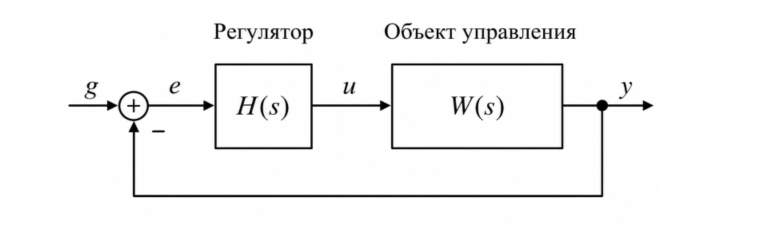
\includegraphics[width=0.85\textwidth]{schema_task1.png}
    \caption{Структурная схема замкнутой системы с пропорциональным регулятором}
    \label{fig:task1_schema}
\end{figure}


\subsection{Передаточные функции системы}

Передаточная функция разомкнутой системы определяется
произведением передаточных функций регулятора
и объекта управления:
\begin{equation*}
    L(s)=H(s)W(s).
\end{equation*}

Подставляя исходные данные, получим:
\begin{equation*}
    L(s)=\frac{1.5K}{0.1s^2+2.2s+1}.
\end{equation*}

Для системы с единичной отрицательной обратной связью
передаточная функция замкнутой системы по задающему
воздействию определяется выражением:
\begin{equation*}
    T(s)=\frac{L(s)}{1+L(s)}.
\end{equation*}

Следовательно:
\begin{equation}
    \boxed{
    T(s)=
    \frac{1.5K}
    {0.1s^2+2.2s+1+1.5K}
    }.
\end{equation}

Передаточная функция замкнутой системы по ошибке
имеет вид:
\begin{equation*}
    W_{g\to e}(s)=\frac{1}{1+L(s)}.
\end{equation*}

После подстановки получим:
\begin{equation}
    \boxed{
    W_{g\to e}(s)=
    \frac{0.1s^2+2.2s+1}
    {0.1s^2+2.2s+1+1.5K}
    }.
\end{equation}

Характеристический полином замкнутой системы:
\begin{equation*}
    D(s)=0.1s^2+2.2s+1+1.5K.
\end{equation*}

При $K\in\{1,5,10\}$ все коэффициенты
характеристического полинома второго порядка
положительны. Следовательно, замкнутая система
асимптотически устойчива для всех рассматриваемых
значений коэффициента усиления.


\subsection{Исследование при постоянном задающем воздействии}

Рассмотрим задающее воздействие:
\begin{equation*}
    g(t)=A=2, \quad G(s)=\frac{2}{s}.
\end{equation*}

Изображение ошибки слежения определяется выражением:
\begin{equation*}
    E(s)=W_{g\to e}(s)G(s).
\end{equation*}

Подставляя передаточную функцию по ошибке, получим:
\begin{equation*}
    E(s)=
    \frac{0.1s^2+2.2s+1}
    {0.1s^2+2.2s+1+1.5K}
    \cdot\frac{2}{s}.
\end{equation*}

Для определения предельного значения установившейся
ошибки воспользуемся теоремой о предельном значении:
\begin{equation*}
    \varepsilon=
    \lim_{t\to\infty}e(t)
    =\lim_{s\to0}sE(s).
\end{equation*}

Тогда:
\begin{equation*}
    \varepsilon=
    \lim_{s\to0}
    \frac{2(0.1s^2+2.2s+1)}
    {0.1s^2+2.2s+1+1.5K}.
\end{equation*}

В результате получим:
\begin{equation}
    \boxed{
    \varepsilon=\frac{2}{1+1.5K}
    }.
\end{equation}

Установившееся значение выходного сигнала:
\begin{equation*}
    y_{\text{уст}}=A-\varepsilon.
\end{equation*}

Результаты расчёта ошибки и выходного сигнала
для различных коэффициентов усиления приведены
в таблице~\ref{tab:task1_constant}.

\begin{table}[H]
    \centering
    \caption{Установившиеся значения выходного сигнала  и ошибки слежения}
    \label{tab:task1_constant}

    \setlength{\tabcolsep}{35pt}

    \begin{tabular}{ccc}
        \toprule
        $K$ & $\varepsilon$ & $y_{\text{уст}}$ \\
        \midrule
        1  & 0.8000 & 1.2000 \\
        5  & 0.2353 & 1.7647 \\
        10 & 0.1250 & 1.8750 \\
        \bottomrule
    \end{tabular}
\end{table}



Для проверки аналитических результатов проводится
моделирование переходных процессов при
$K=1$, $K=5$ и $K=10$.

% -----------------------------------------------------------
% ГРАФИК 1 - Выходной сигнал y(t), g(t) = 2
% -----------------------------------------------------------
\begin{figure}[H]
    \centering
    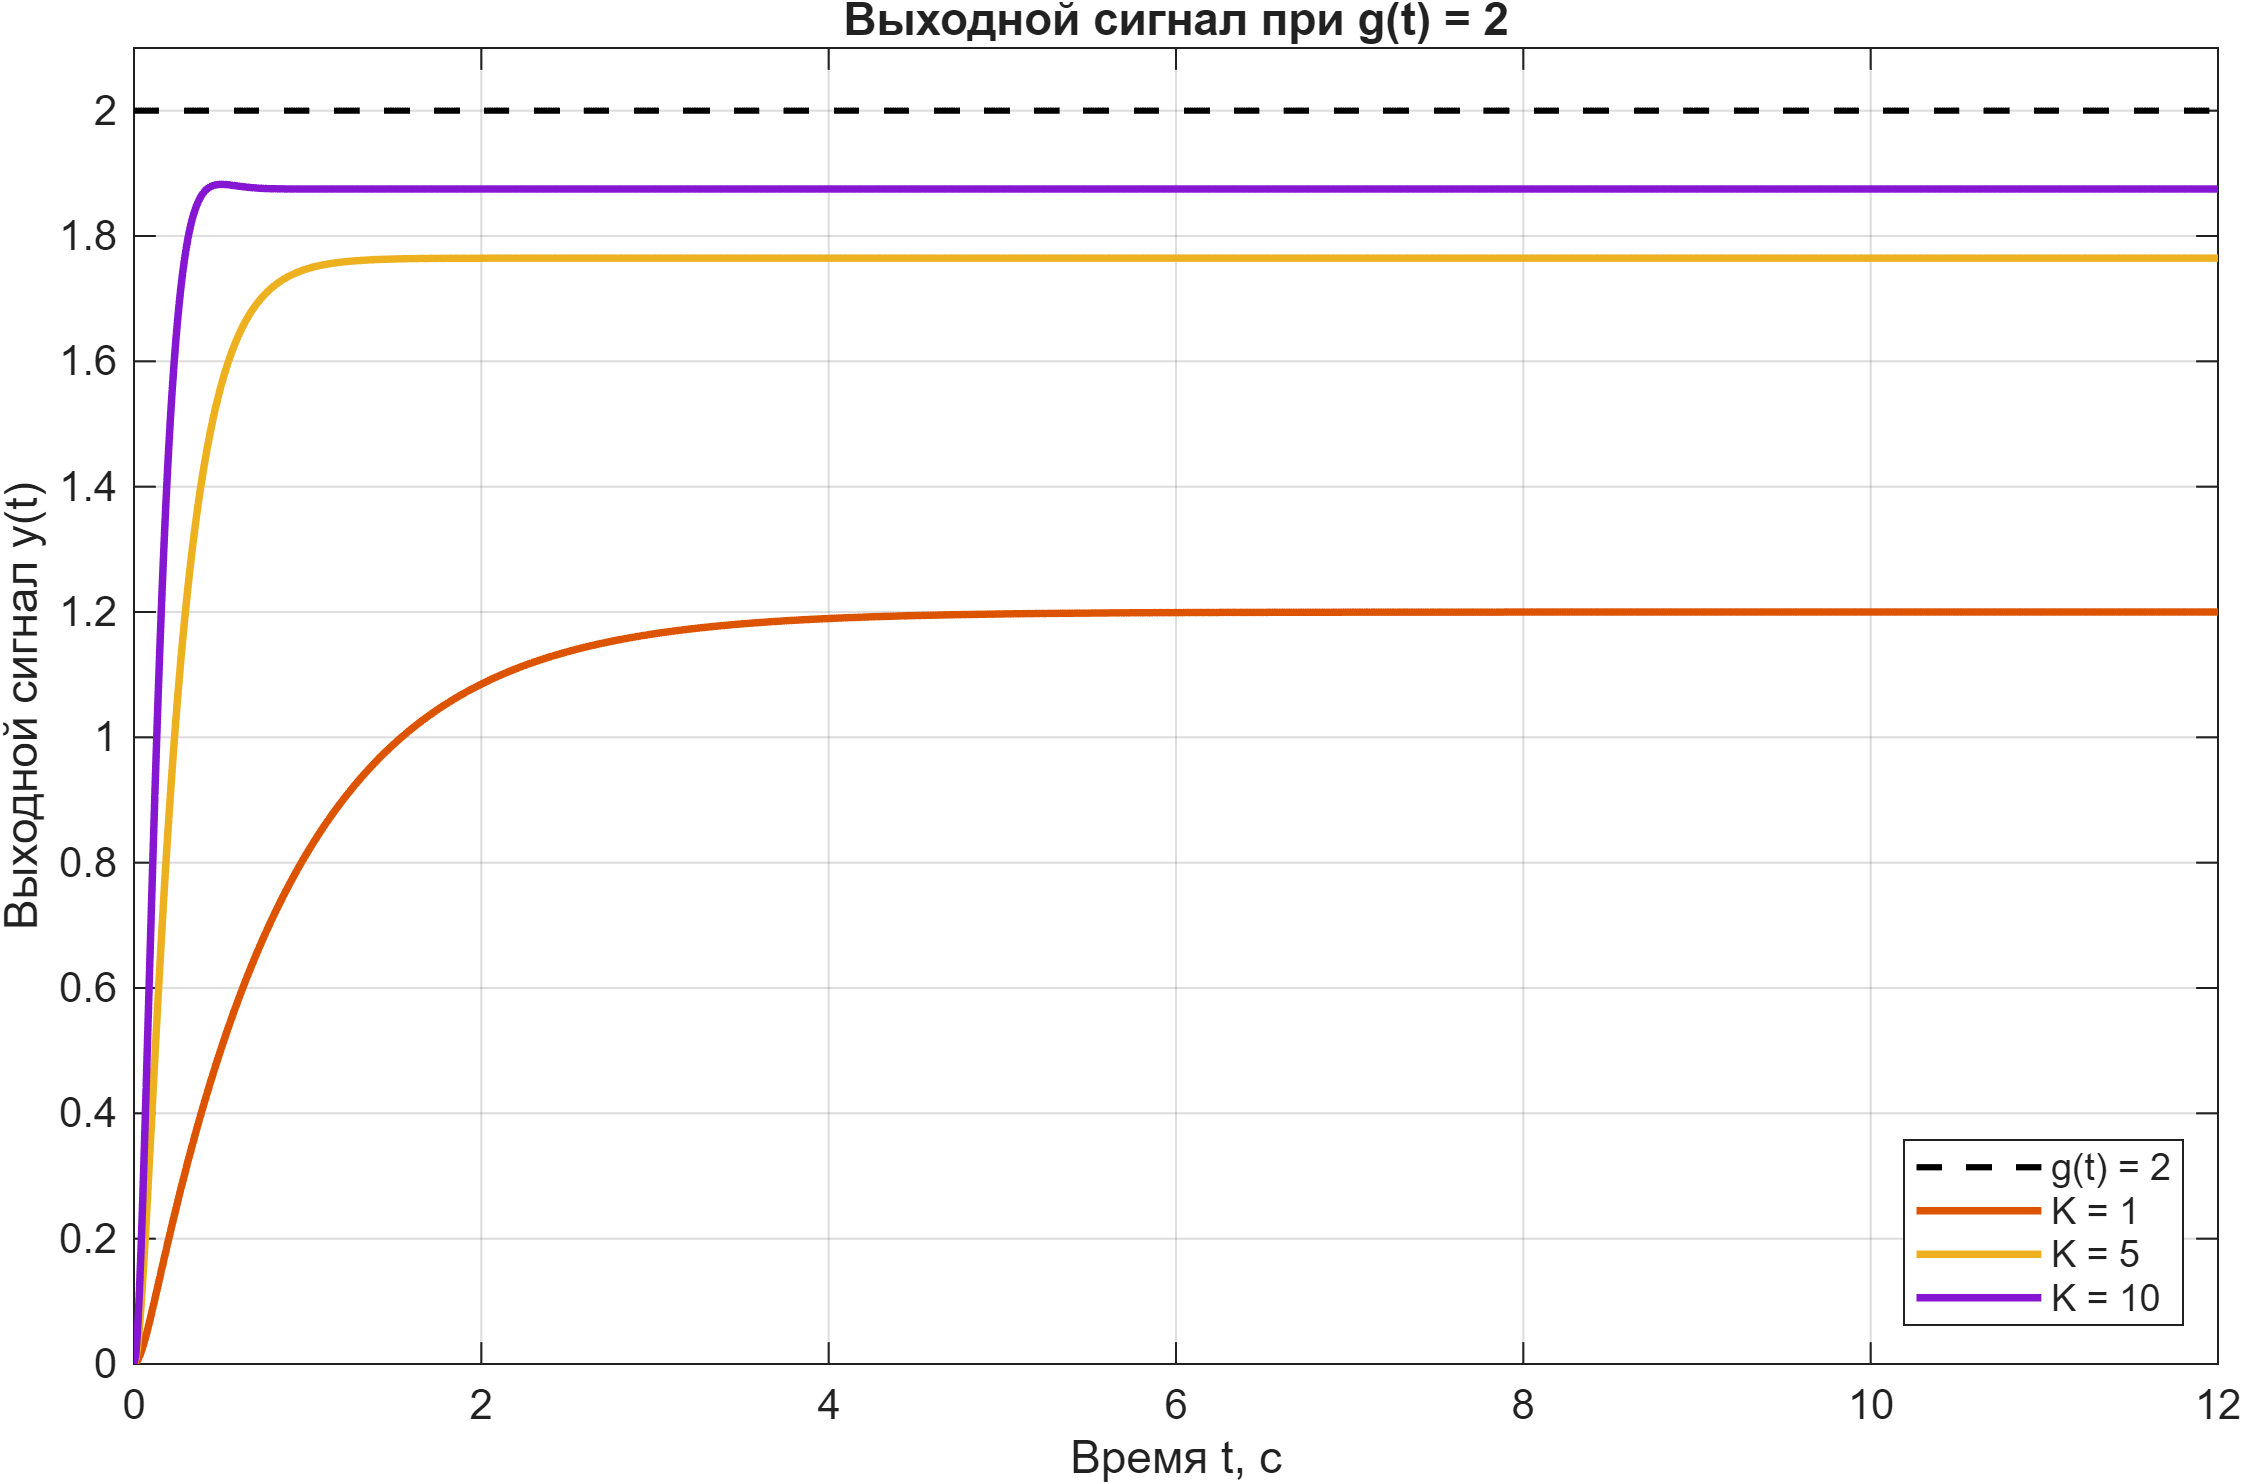
\includegraphics[width=0.85\textwidth]{res1/Lab5_Task1_Figure1.png}
    \caption{Переходные процессы выходного сигнала
    при $g(t)=2$}
    \label{fig:task1_y_constant}
\end{figure}

% -----------------------------------------------------------
% ГРАФИК 2 - Ошибка слежения e(t), g(t) = 2
% -----------------------------------------------------------
\begin{figure}[H]
    \centering
    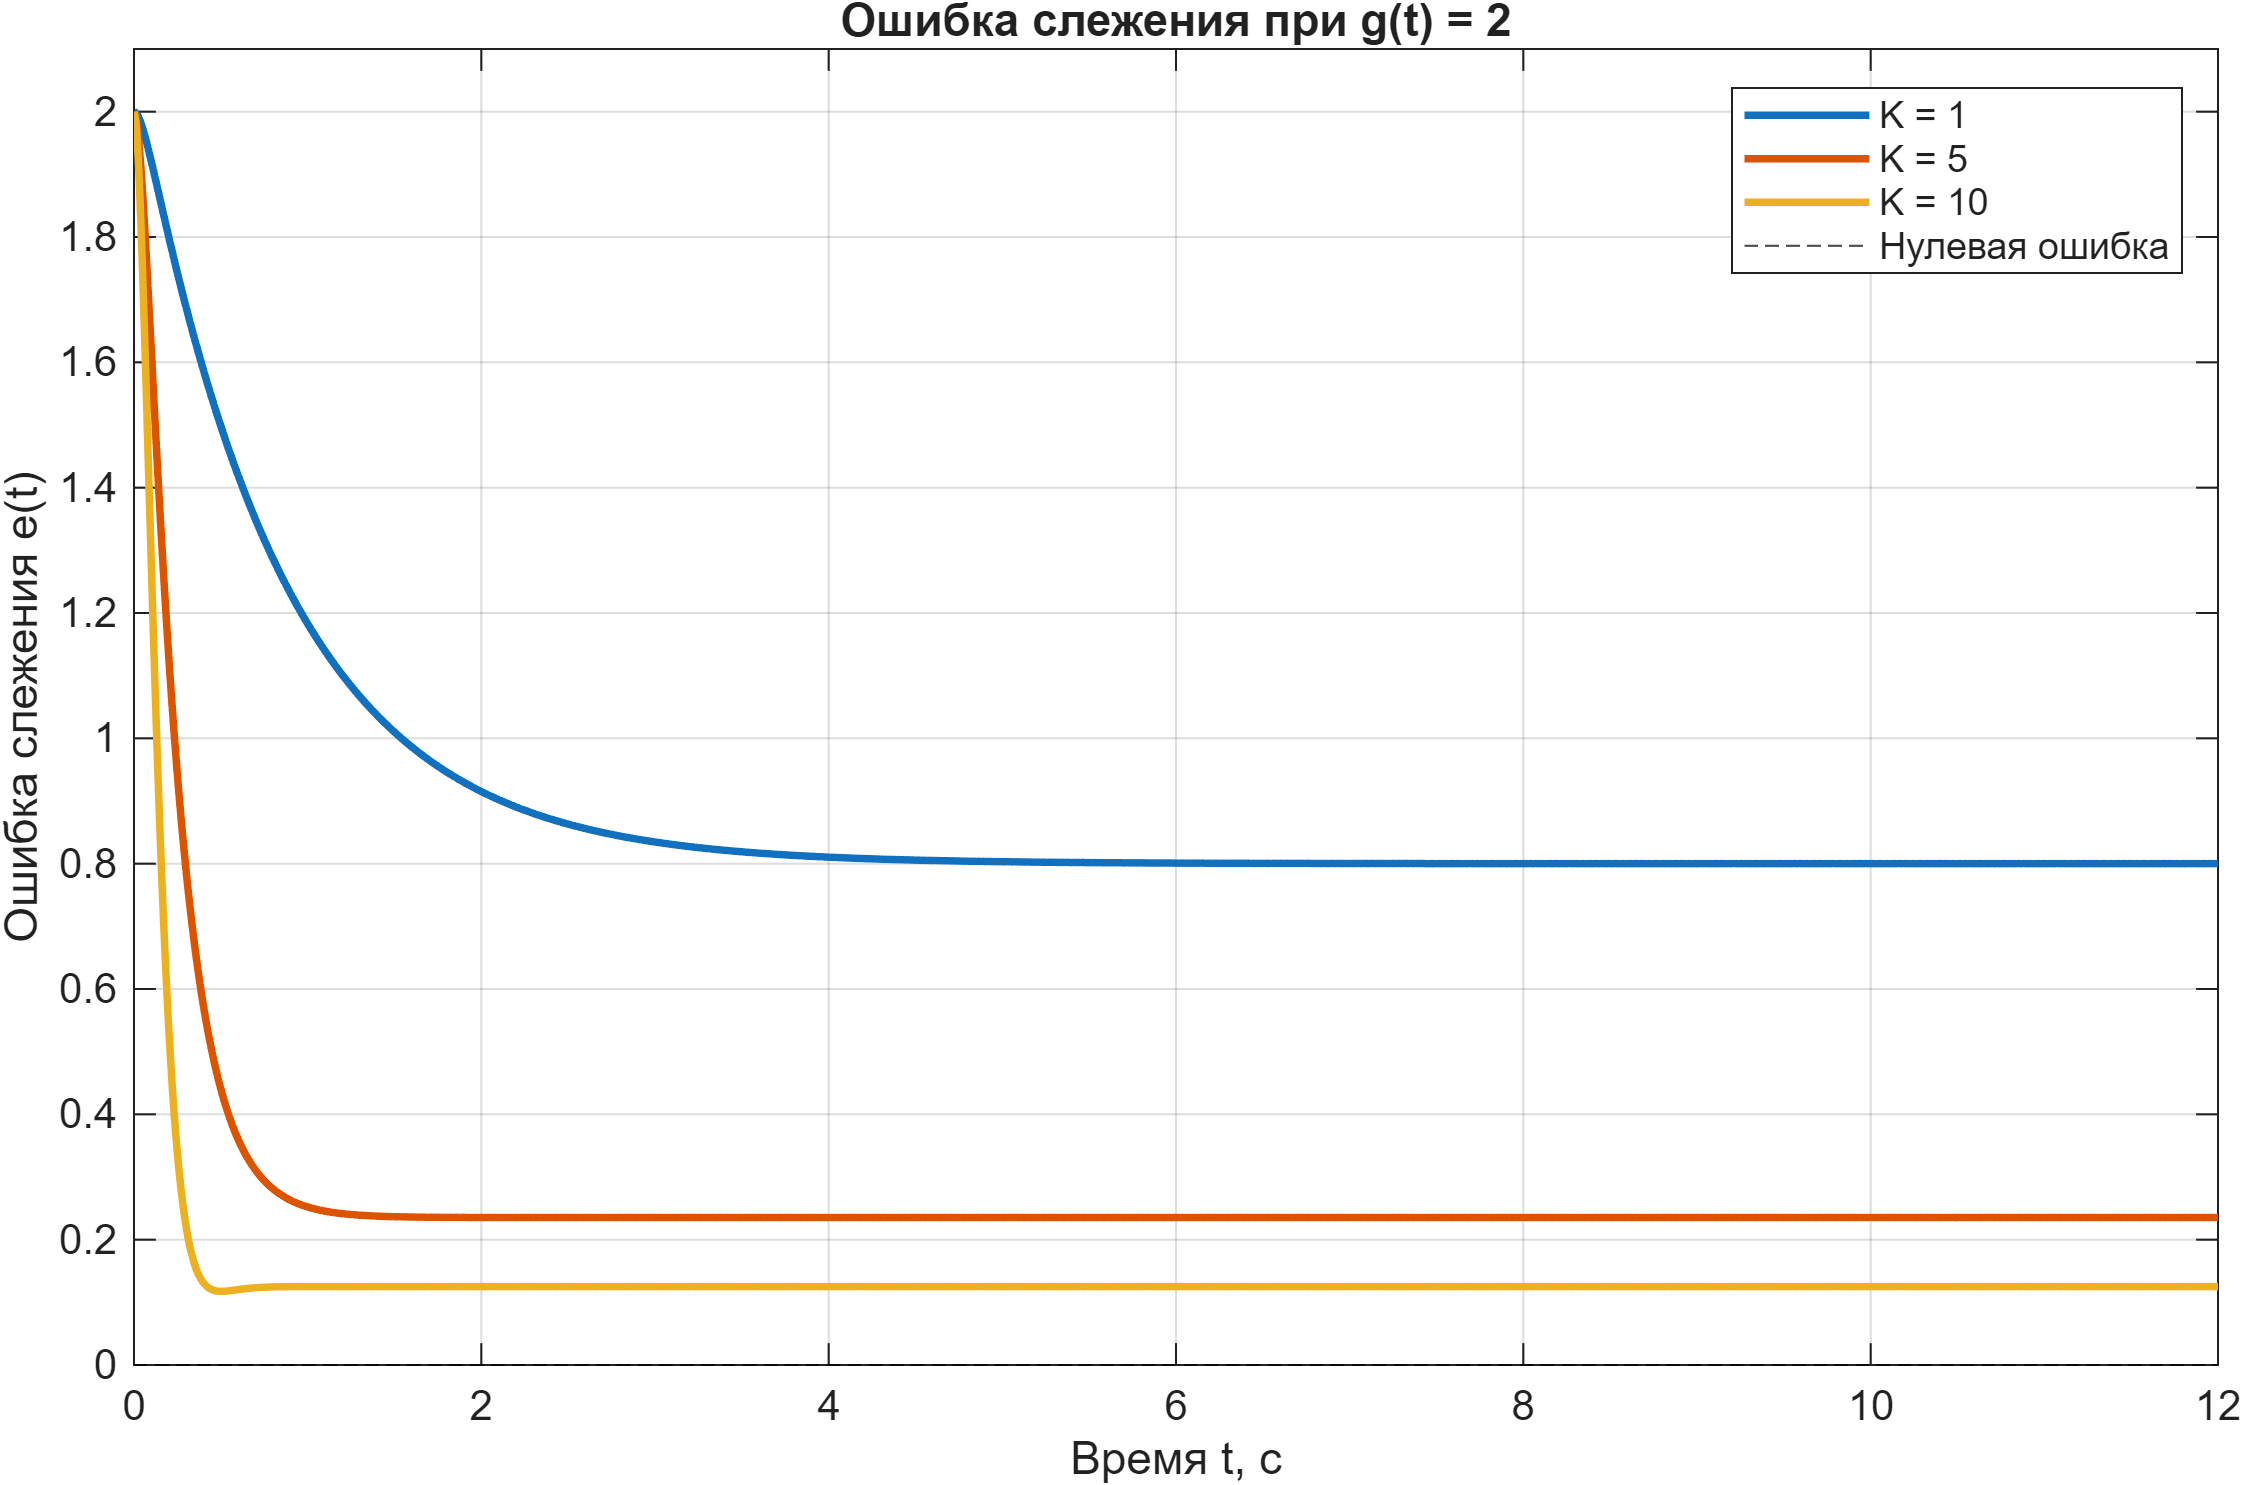
\includegraphics[width=0.85\textwidth]{res1/Lab5_Task1_Figure2.png}
    \caption{Переходные процессы ошибки слежения
    при $g(t)=2$}
    \label{fig:task1_e_constant}
\end{figure}

При увеличении коэффициента усиления $K$
установившаяся ошибка слежения уменьшается.
Однако при всех рассматриваемых значениях $K$
ошибка остаётся отличной от нуля.

Это объясняется тем, что разомкнутая система
не содержит интегрирующих звеньев и обладает
нулевым порядком астатизма.


\subsection{Исследование при линейно возрастающем
задающем воздействии}

Рассмотрим задающее воздействие:
\begin{equation*}
    g(t)=Vt=4t, \quad G(s)=\frac{4}{s^2}.
\end{equation*}

Изображение ошибки слежения:
\begin{equation*}
    E(s)=W_{g\to e}(s)G(s).
\end{equation*}

После подстановки:
\begin{equation*}
    E(s)=
    \frac{0.1s^2+2.2s+1}
    {0.1s^2+2.2s+1+1.5K}
    \cdot\frac{4}{s^2}.
\end{equation*}

Для исследования установившейся составляющей ошибки
разложим передаточную функцию по ошибке
в ряд Тейлора в окрестности $s=0$:
\begin{equation*}
    W_{g\to e}(s)=c_0+c_1s+O(s^2).
\end{equation*}

Первый коэффициент ошибки:
\[
    c_0=W_{g\to e}(0)
    =\frac{1}{1+1.5K}.
\]

Второй коэффициент:
\[
    c_1=
    \left.
    \frac{dW_{g\to e}(s)}{ds}
    \right|_{s=0}
    =
    \frac{3.3K}{(1+1.5K)^2}.
\]

Для линейного задающего воздействия
$g(t)=4t$ установившаяся составляющая ошибки
определяется выражением:
\[
    e_y(t)=c_0g(t)+c_1\dot{g}(t).
\]

Поскольку $\dot{g}(t)=4$, получим:
\begin{equation}
    \boxed{
    e_y(t)=
    \frac{4}{1+1.5K}t+
    \frac{13.2K}{(1+1.5K)^2}
    }.
\end{equation}

Для различных значений коэффициента усиления:

\[
\begin{aligned}
K=1:&\quad e_y(t)=1.6t+2.112,\\
K=5:&\quad e_y(t)\approx 0.4706t+0.9135,\\
K=10:&\quad e_y(t)=0.25t+0.5156.
\end{aligned}
\]

Из полученных выражений видно, что ошибка
слежения неограниченно возрастает при
$t\to\infty$.

Увеличение коэффициента усиления $K$
уменьшает скорость роста ошибки,
но не обеспечивает её полного устранения.


Для подтверждения полученных результатов
проводится моделирование переходных процессов
при трёх значениях коэффициента усиления.

% -----------------------------------------------------------
% ГРАФИК 3 - Выходной сигнал y(t), g(t) = 4t
% -----------------------------------------------------------
\begin{figure}[H]
    \centering
    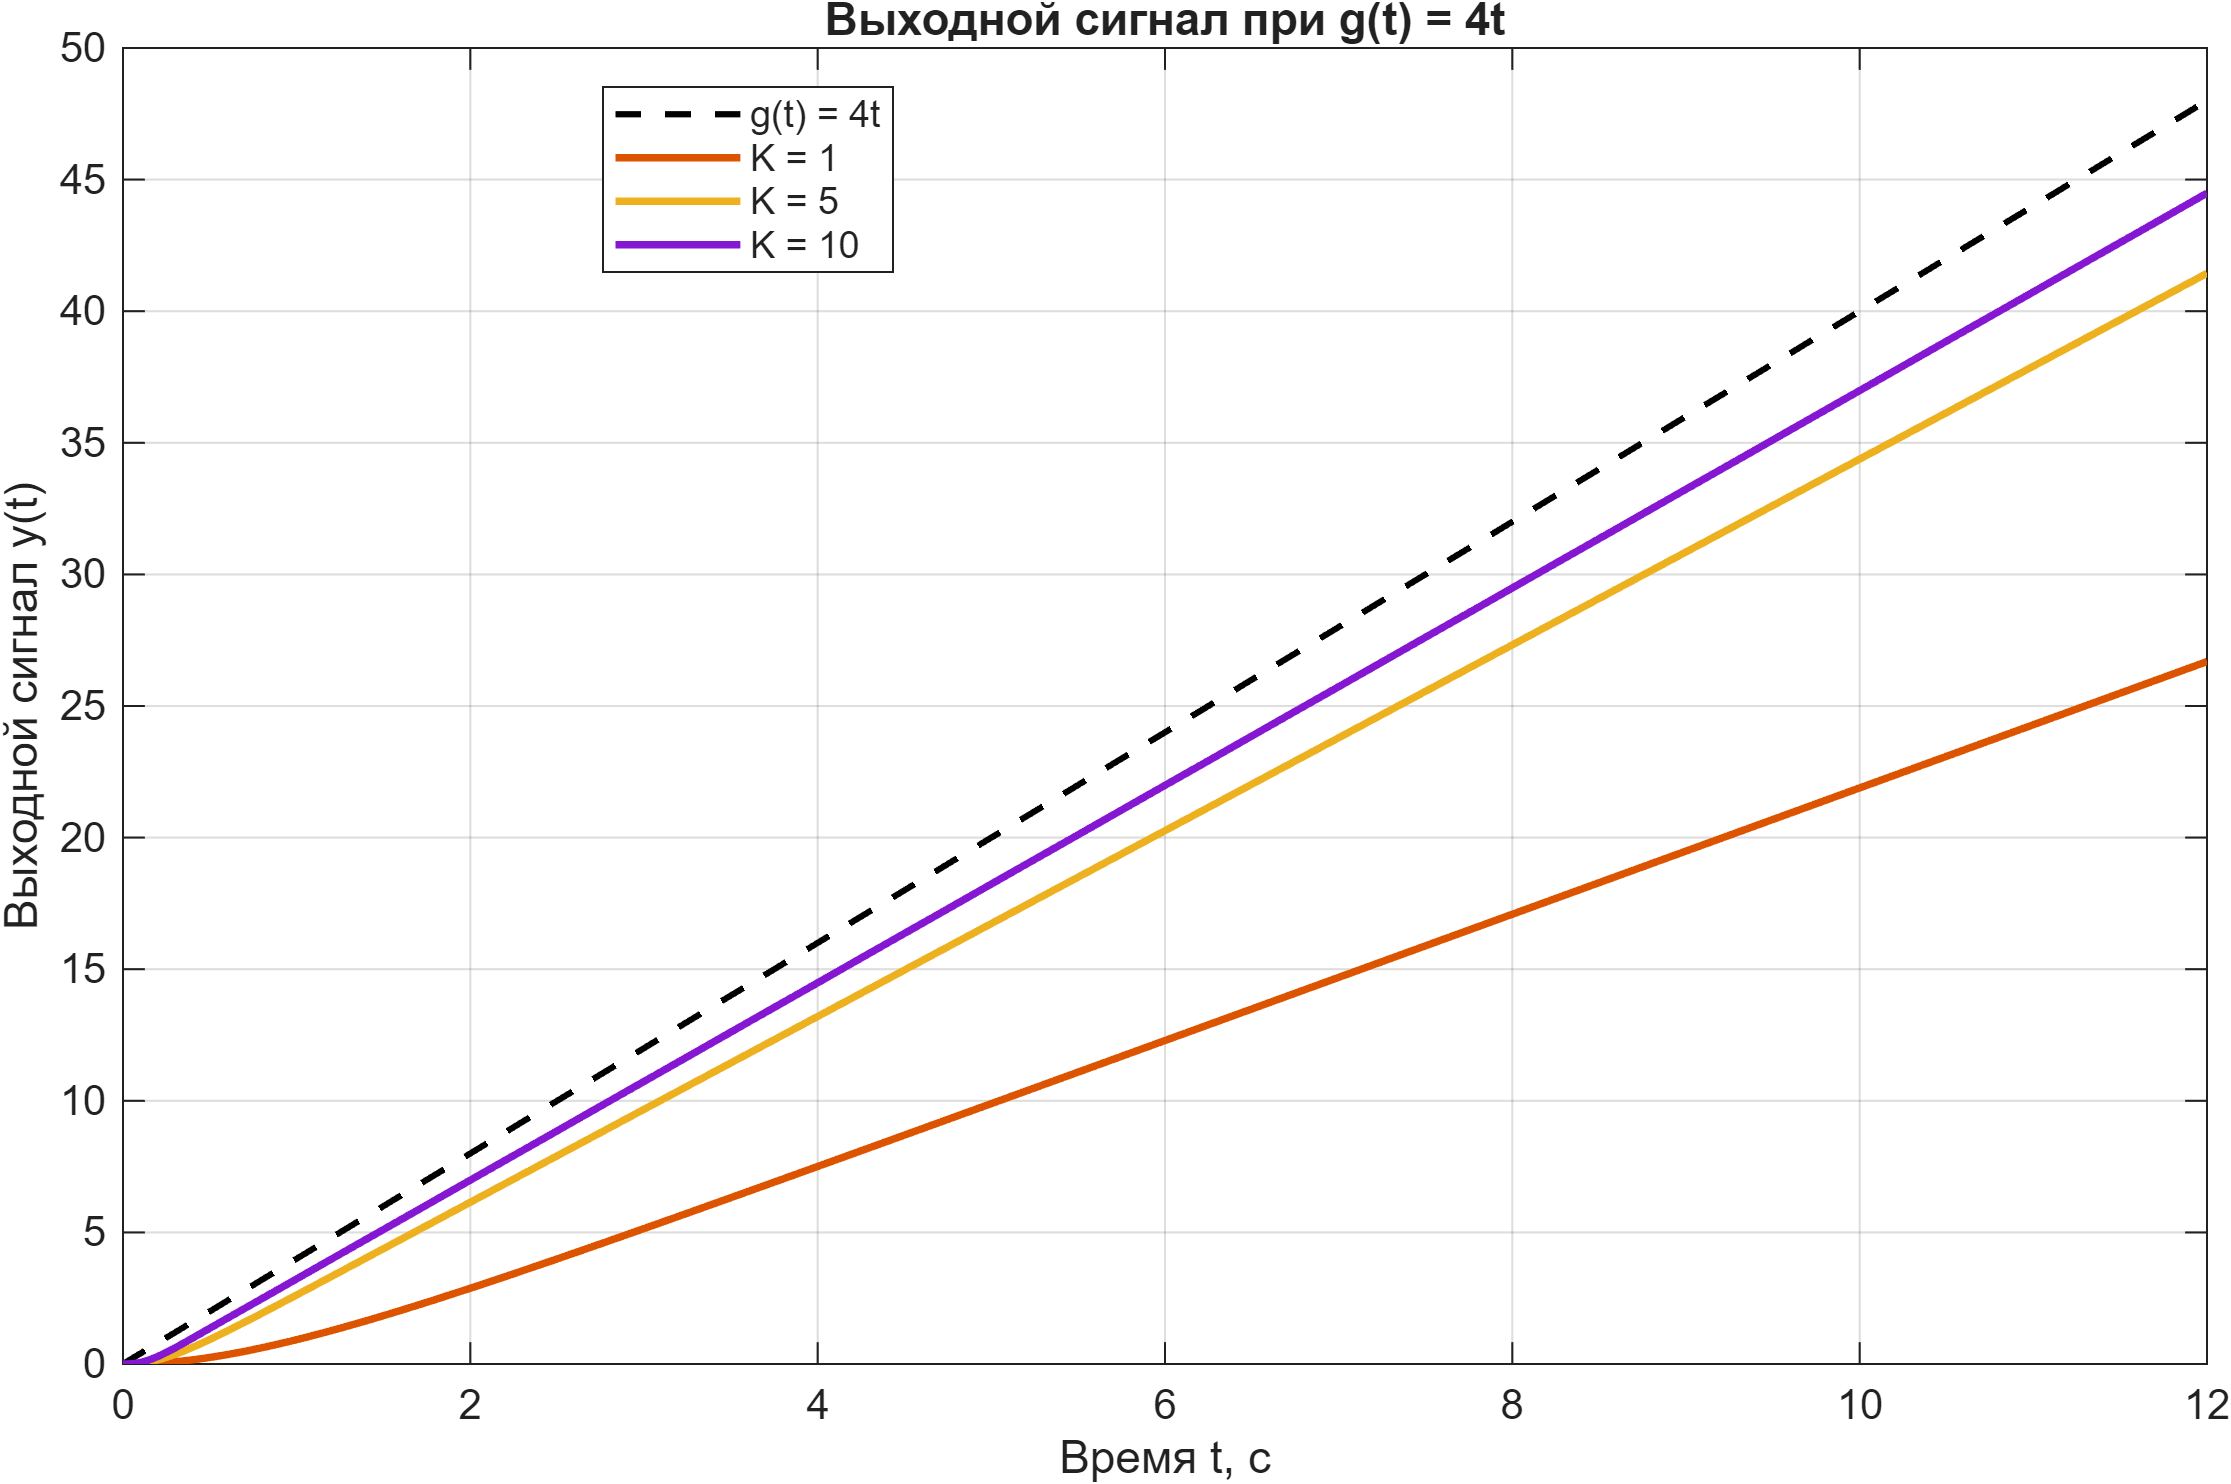
\includegraphics[width=0.85\textwidth]{res1/Lab5_Task1_Figure3.png}
    \caption{Переходные процессы выходного сигнала
    при $g(t)=4t$}
    \label{fig:task1_y_ramp}
\end{figure}

% -----------------------------------------------------------
% ГРАФИК 4 - Ошибка слежения e(t), g(t) = 4t
% -----------------------------------------------------------
\begin{figure}[H]
    \centering
    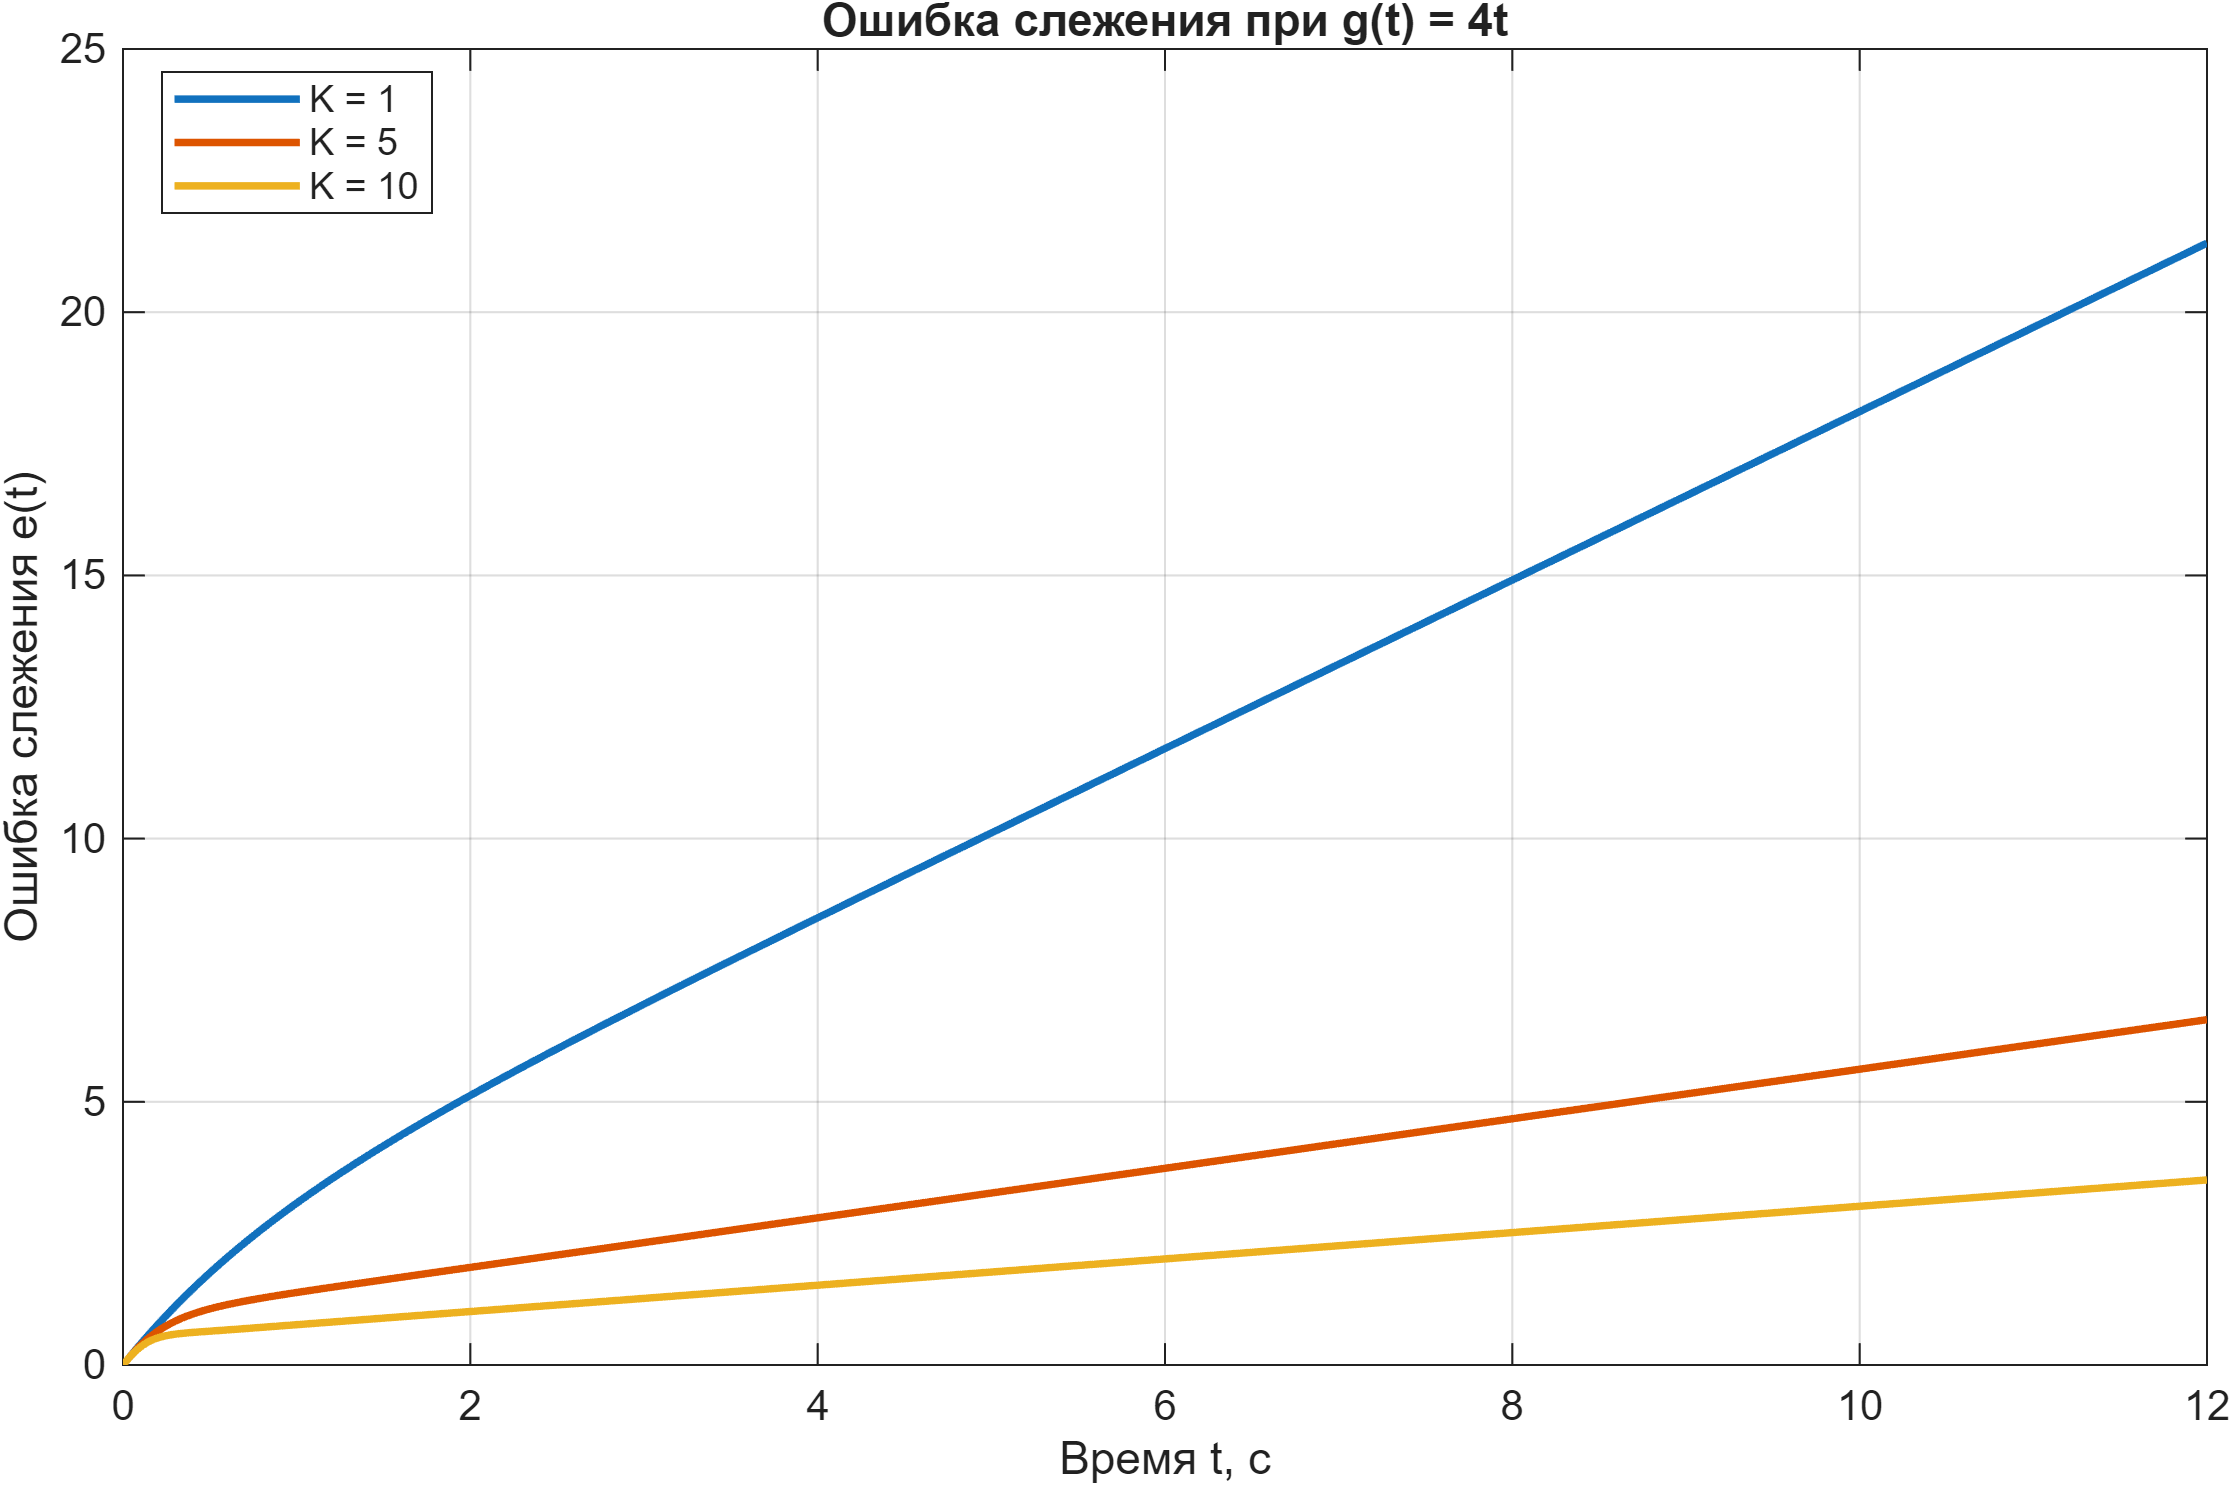
\includegraphics[width=0.85\textwidth]{res1/Lab5_Task1_Figure4.png}
    \caption{Переходные процессы ошибки слежения
    при $g(t)=4t$}
    \label{fig:task1_e_ramp}
\end{figure}


\subsection{Вывод по заданию 1}

В ходе выполнения задания исследованы точностные
свойства замкнутой системы управления
с пропорциональным регулятором.

При постоянном задающем воздействии установлено,
что увеличение коэффициента усиления $K$
приводит к уменьшению установившейся ошибки.
Однако ошибка не становится равной нулю.

При линейно возрастающем задающем воздействии
ошибка слежения неограниченно возрастает.
Увеличение коэффициента усиления позволяет
уменьшить скорость её роста.

Таким образом, система с пропорциональным
регулятором обладает нулевым порядком астатизма
и не обеспечивает нулевую установившуюся ошибку
при рассматриваемых задающих воздействиях.



% ===========================================================
% ЗАДАНИЕ 2. ИНТЕГРАЛЬНЫЙ РЕГУЛЯТОР
% ===========================================================

\newpage
\section{Задание 2. Интегральный регулятор}

\subsection{Исходные данные}

В соответствии с вариантом 3 передаточная функция
объекта управления имеет вид:
\begin{equation*}
    W(s)=\frac{1.5}{0.1s^2+2.2s+1}.
\end{equation*}

В системе используется интегральный регулятор
с передаточной функцией:
\begin{equation}
    \boxed{
    H(s)=\frac{K}{s}
    },
    \qquad K\in\{1,5,10\}.
\end{equation}

Рассматривается замкнутая система с единичной
отрицательной обратной связью.

Исследуются три вида задающего воздействия:
\begin{itemize}
    \item постоянное воздействие $g(t)=2$;
    \item линейно возрастающее воздействие $g(t)=4t$;
    \item квадратично возрастающее воздействие
    $g(t)=0.2t^2$.
\end{itemize}

Ошибка слежения определяется выражением:
\[
    e(t)=g(t)-y(t).
\]

Структурная схема системы соответствует схеме
с единичной отрицательной обратной связью.

% -----------------------------------------------------------
% СТРУКТУРНАЯ СХЕМА
% -----------------------------------------------------------
Раскомментировать после добавления изображения.

\begin{figure}[H]
    \centering
    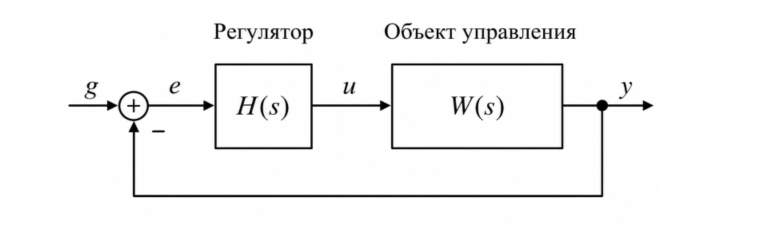
\includegraphics[width=0.85\textwidth]{schema_task1.png}
    \caption{Структурная схема замкнутой системы с интегральным регулятором}
    \label{fig:task2_schema}
\end{figure}


\subsection{Передаточные функции системы}

Передаточная функция разомкнутой системы:
\[
    L(s)=H(s)W(s).
\]

Подставляя исходные данные, получим:
\[
    L(s)=
    \frac{1.5K}{s(0.1s^2+2.2s+1)}.
\]

Передаточная функция замкнутой системы
по задающему воздействию:
\[
    T(s)=\frac{L(s)}{1+L(s)}.
\]

Следовательно:
\begin{equation}
    \boxed{
    T(s)=
    \frac{1.5K}
    {0.1s^3+2.2s^2+s+1.5K}
    }.
\end{equation}

Передаточная функция замкнутой системы
по ошибке:
\[
    W_{g\to e}(s)=\frac{1}{1+L(s)}.
\]

После преобразования:
\begin{equation}
    \boxed{
    W_{g\to e}(s)=
    \frac{0.1s^3+2.2s^2+s}
    {0.1s^3+2.2s^2+s+1.5K}
    }.
\end{equation}

Характеристический полином замкнутой системы:
\[
    D(s)=0.1s^3+2.2s^2+s+1.5K.
\]

Для определения устойчивости воспользуемся
критерием Гурвица. Для полинома третьей степени
необходимо выполнение условий положительности
коэффициентов и неравенства:
\[
    2.2\cdot 1>0.1\cdot1.5K.
\]

Отсюда:
\[
    K<\frac{44}{3}\approx14.67.
\]

Таким образом, при $K=1$, $K=5$ и $K=10$
замкнутая система асимптотически устойчива.

Наличие интегратора в прямом контуре
обеспечивает первый порядок астатизма системы.


\subsection{Исследование при постоянном
задающем воздействии}

Рассмотрим постоянное задающее воздействие:
\[
    g(t)=A=2,
    \qquad G(s)=\frac{2}{s}.
\]

Изображение ошибки слежения:
\[
    E(s)=W_{g\to e}(s)G(s).
\]

После подстановки:
\[
    E(s)=
    \frac{0.1s^3+2.2s^2+s}
    {0.1s^3+2.2s^2+s+1.5K}
    \cdot\frac{2}{s}.
\]

Для определения предельного значения
установившейся ошибки используем
теорему о предельном значении:
\[
    \varepsilon=
    \lim_{t\to\infty}e(t)
    =\lim_{s\to0}sE(s).
\]

Тогда:
\[
    \varepsilon=
    \lim_{s\to0}
    \frac{2(0.1s^3+2.2s^2+s)}
    {0.1s^3+2.2s^2+s+1.5K}.
\]

В результате:
\begin{equation}
    \boxed{\varepsilon=0}.
\end{equation}

Следовательно, при всех рассматриваемых
значениях коэффициента усиления установившаяся
ошибка равна нулю.

Установившееся значение выходного сигнала:
\[
    y_{\text{уст}}=A-\varepsilon=2.
\]

Результаты аналитического расчёта
представлены в таблице~\ref{tab:task2_constant}.

\begin{table}[H]
    \centering
    \caption{Установившиеся значения при $g(t)=2$}
    \label{tab:task2_constant}

    \setlength{\tabcolsep}{35pt}

    \begin{tabular}{ccc}
        \toprule
        $K$ & $\varepsilon$ & $y_{\text{уст}}$ \\
        \midrule
        1  & 0 & 2 \\
        5  & 0 & 2 \\
        10 & 0 & 2 \\
        \bottomrule
    \end{tabular}
\end{table}

Для проверки аналитических результатов
проводится моделирование переходных процессов
при трёх значениях коэффициента усиления.

% -----------------------------------------------------------
% ГРАФИК 1 - y(t), g(t) = 2
% -----------------------------------------------------------
\begin{figure}[H]
    \centering
    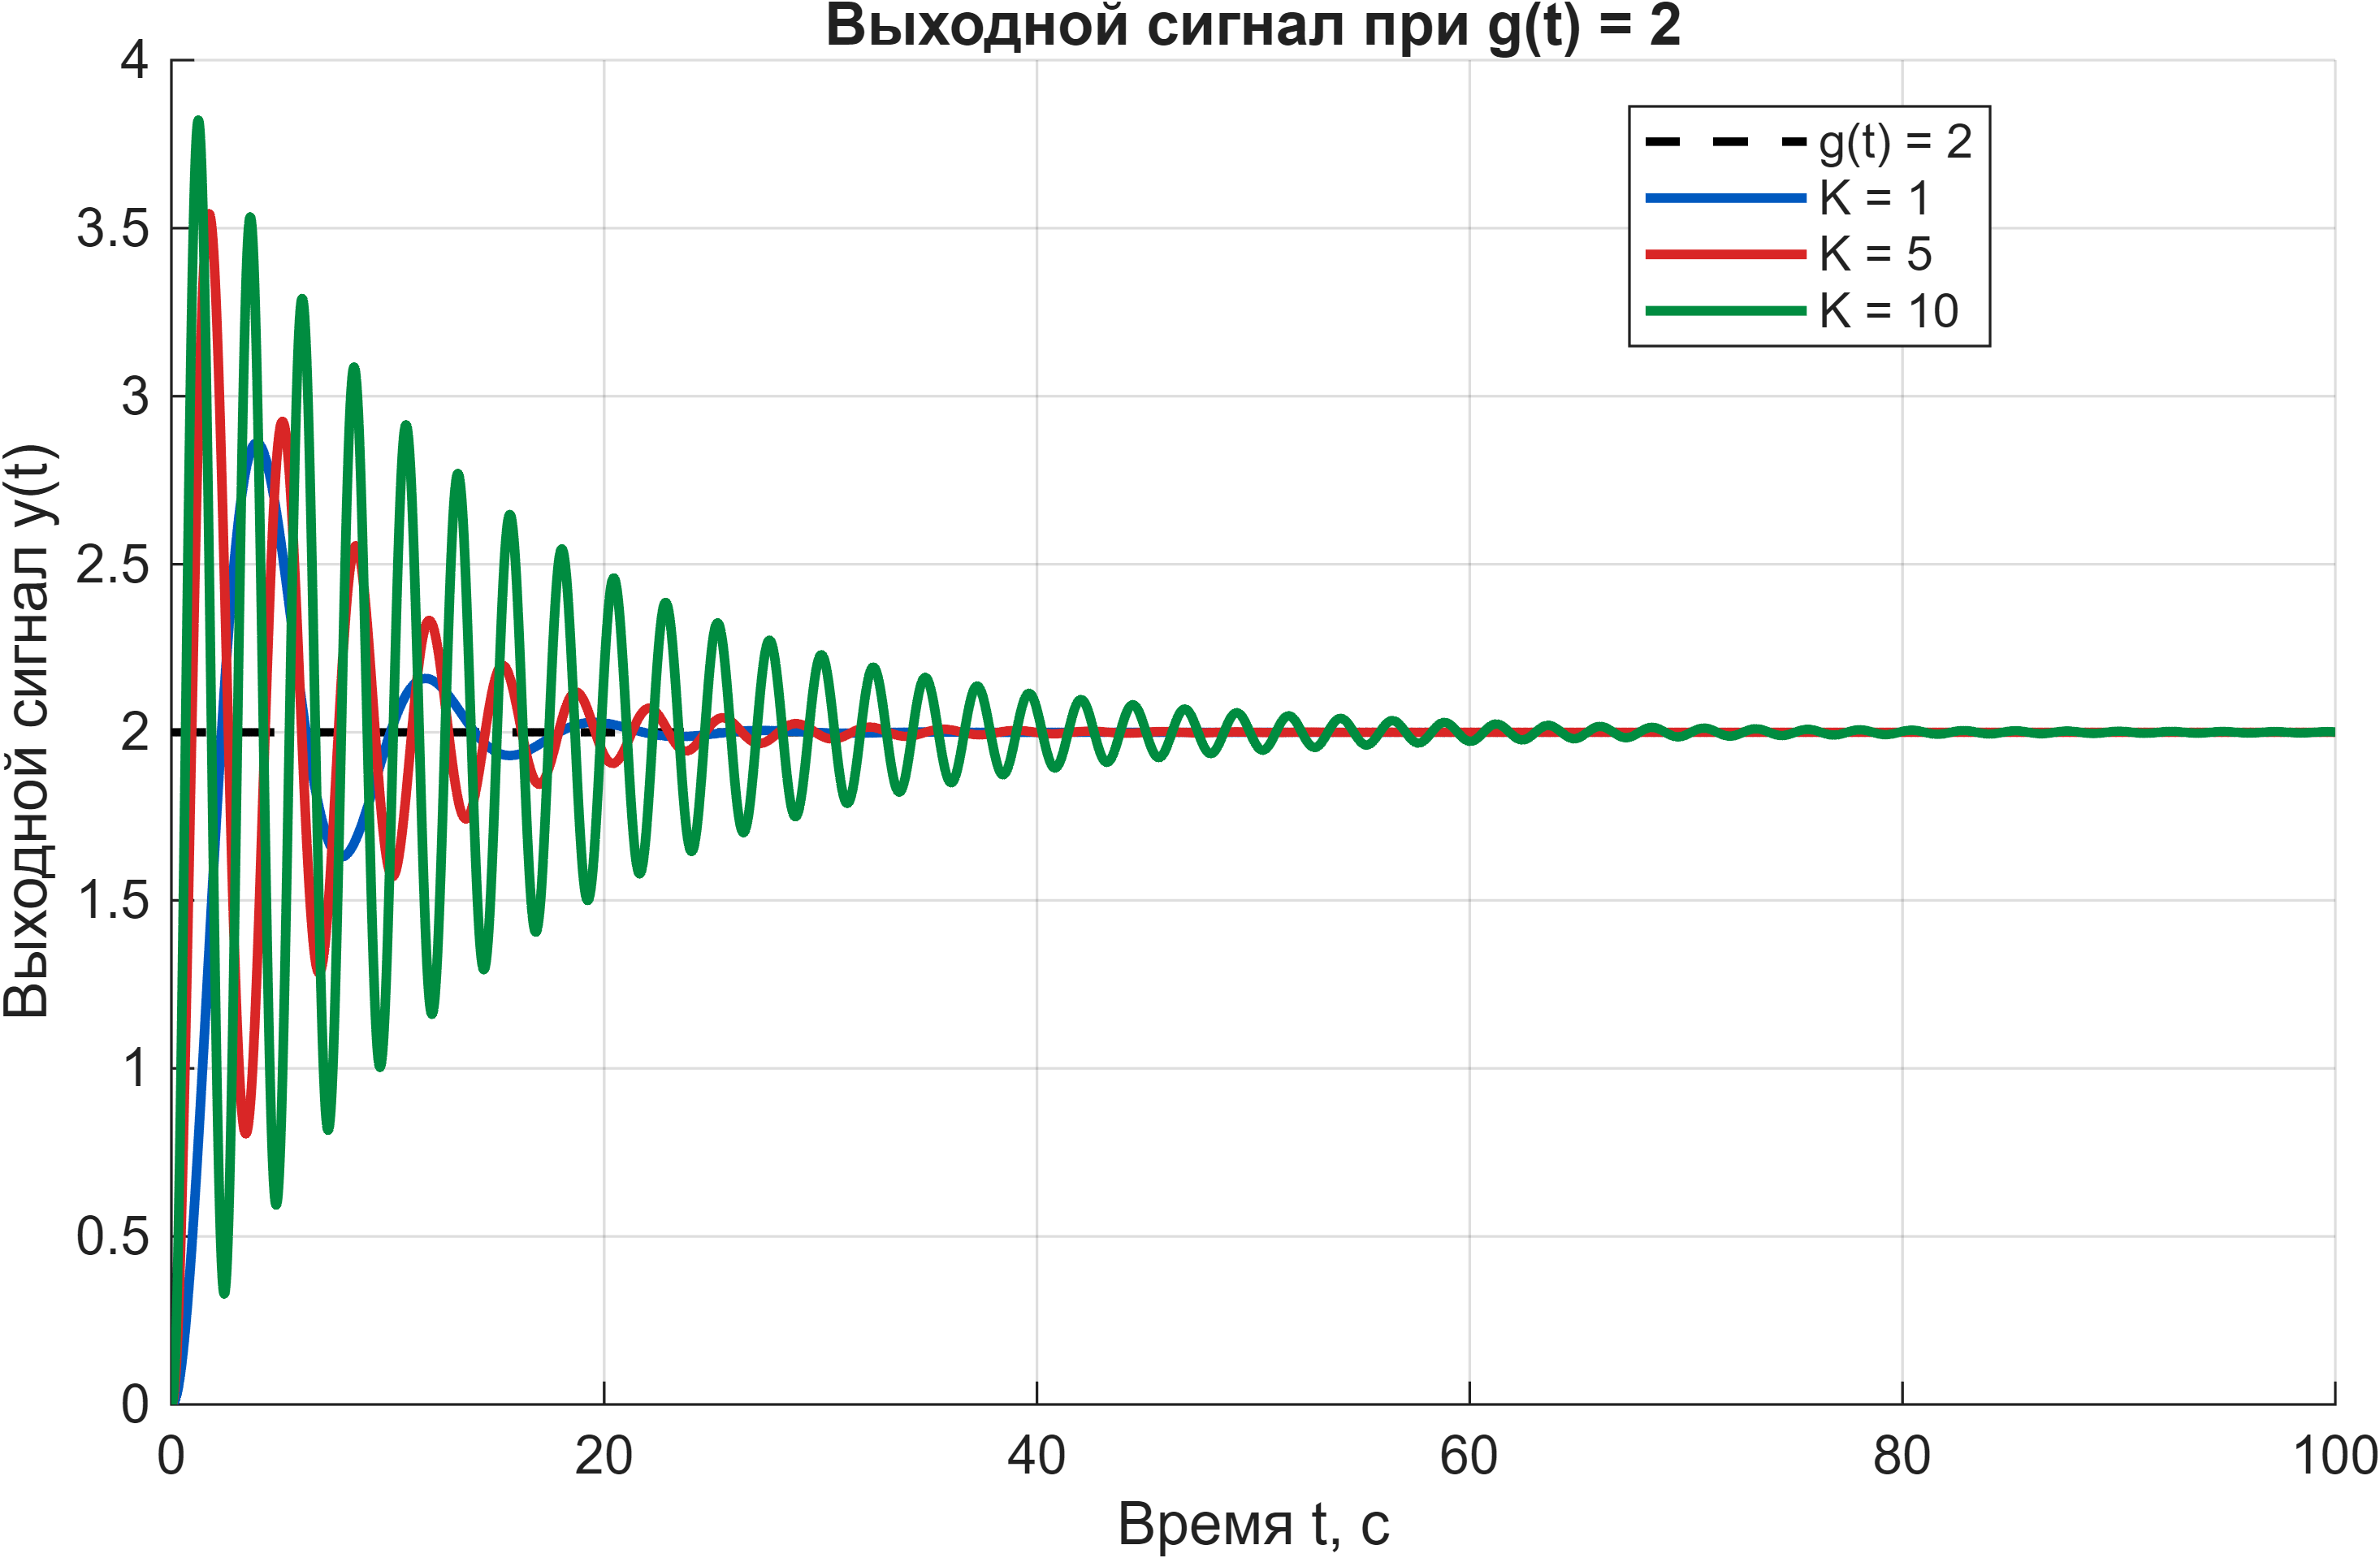
\includegraphics[width=0.85\textwidth]{res2/Lab5_Task2_Figure1.png}
    \caption{Переходные процессы выходного сигнала
    при $g(t)=2$}
    \label{fig:task2_y_constant}
\end{figure}

% -----------------------------------------------------------
% ГРАФИК 2 - e(t), g(t) = 2
% -----------------------------------------------------------
\begin{figure}[H]
    \centering
    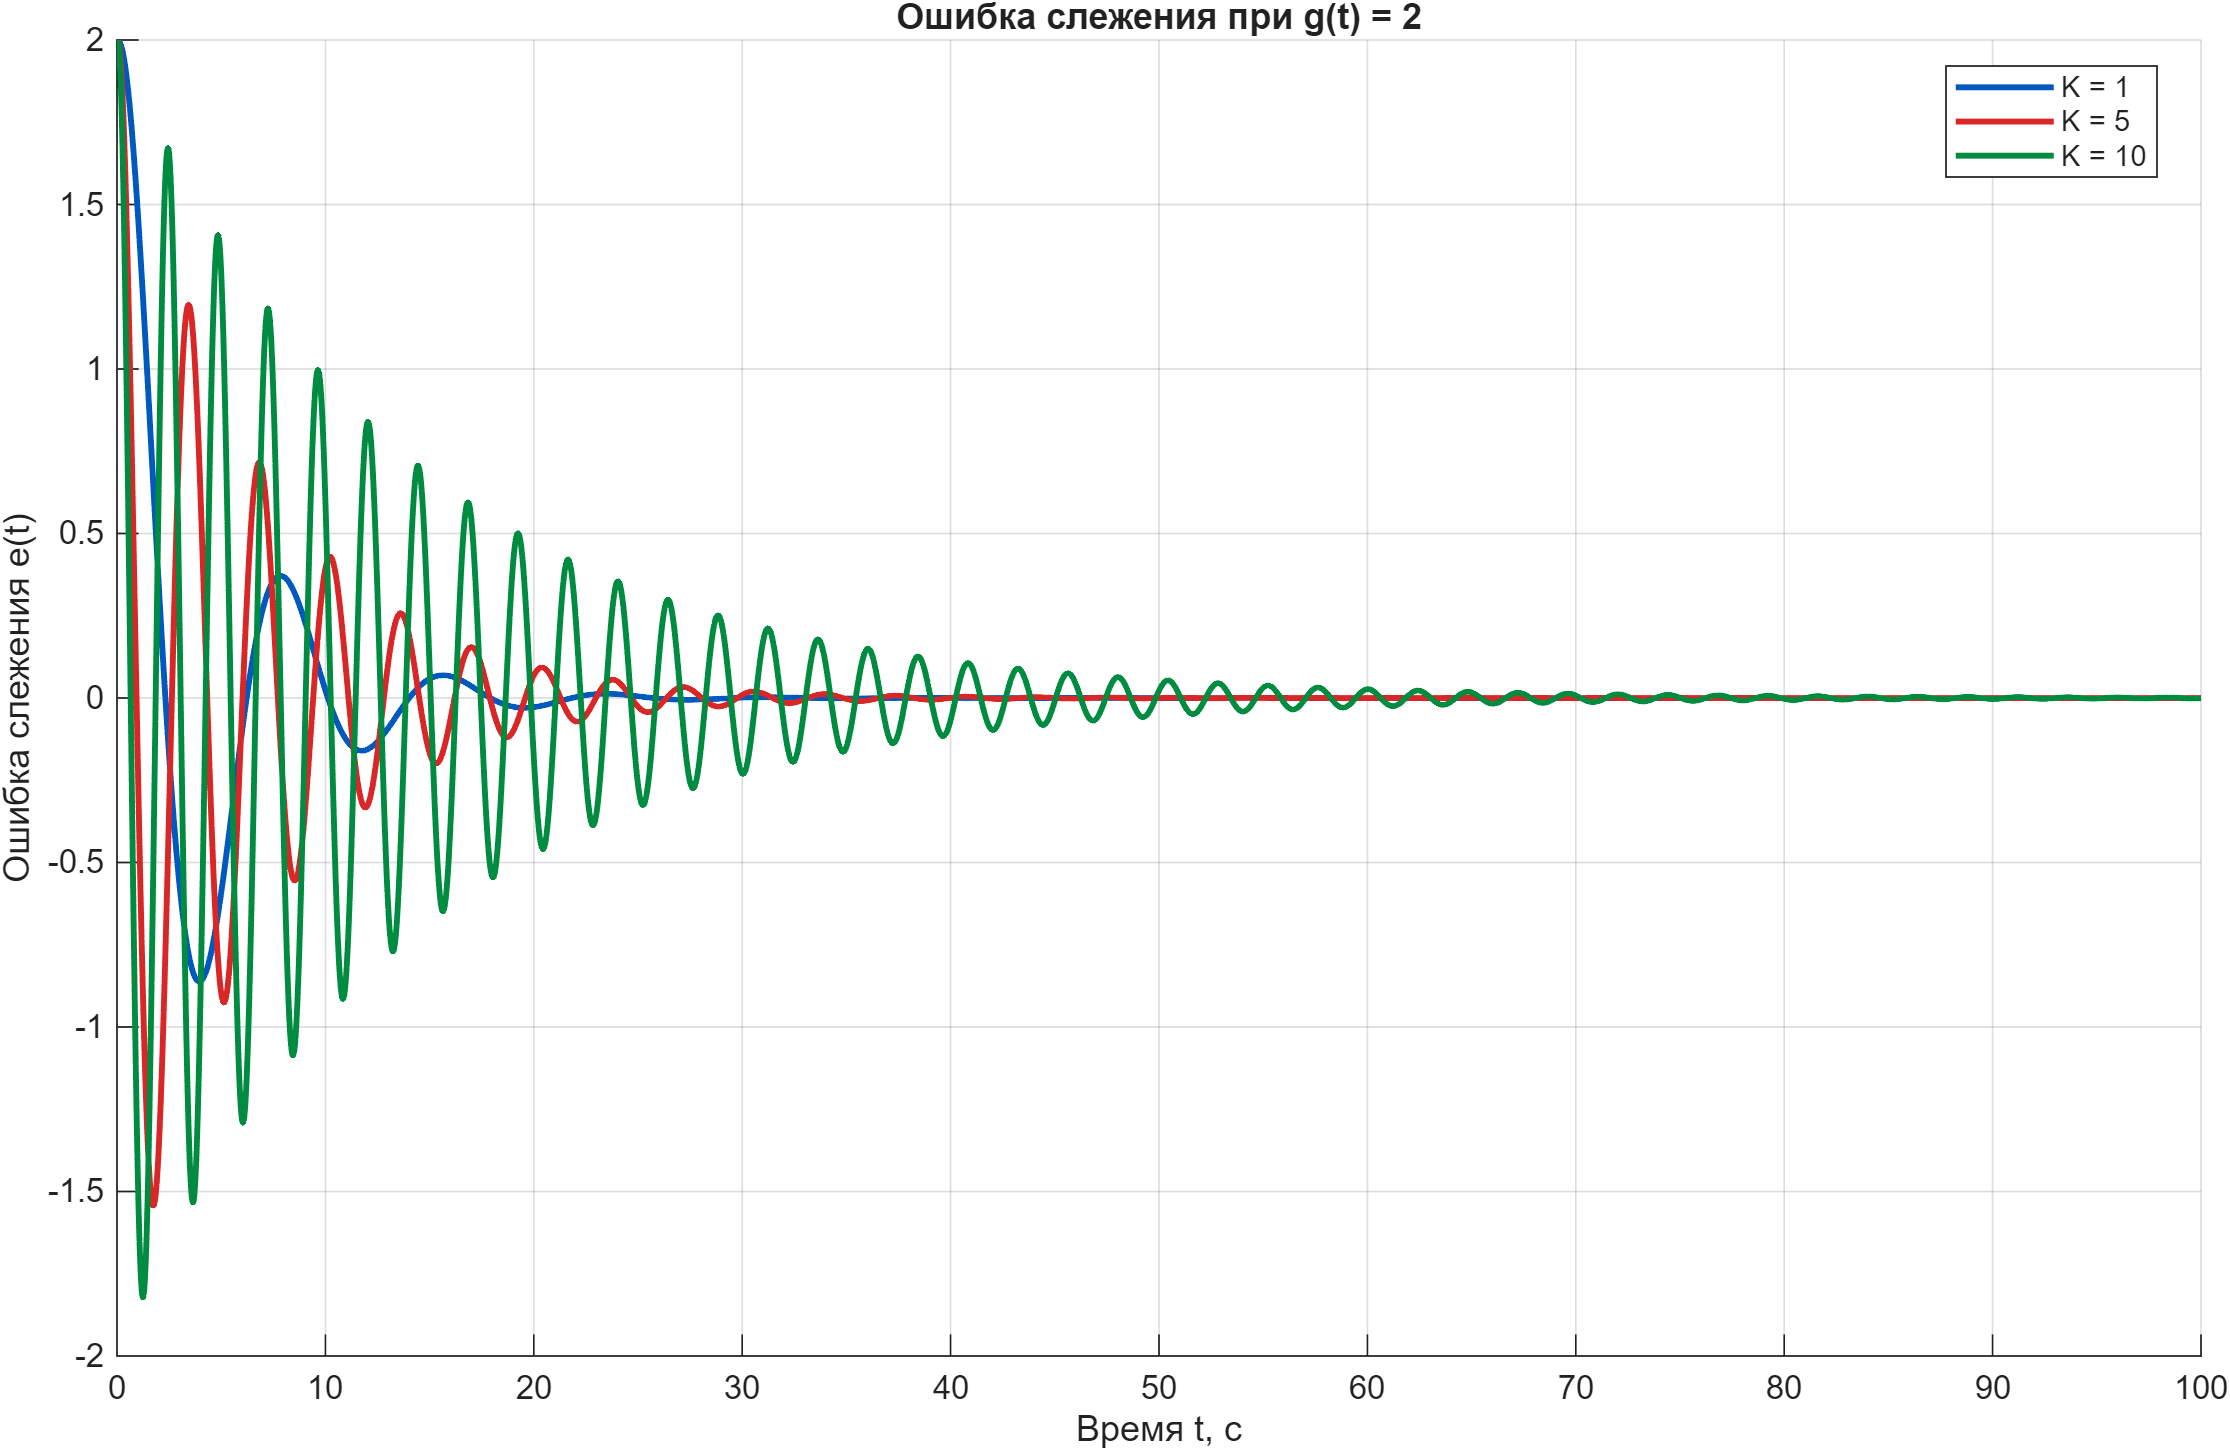
\includegraphics[width=0.85\textwidth]{res2/Lab5_Task2_Figure2.png}
    \caption{Переходные процессы ошибки слежения
    при $g(t)=2$}
    \label{fig:task2_e_constant}
\end{figure}

Благодаря наличию интегрального регулятора
система обеспечивает нулевую установившуюся
ошибку при постоянном задающем воздействии.

Изменение коэффициента усиления влияет
на характер переходного процесса,
но не изменяет предельное значение ошибки.


\subsection{Исследование при линейно возрастающем
задающем воздействии}

Рассмотрим задающее воздействие:
\[
    g(t)=Vt=4t,
    \qquad G(s)=\frac{4}{s^2}.
\]

Изображение ошибки слежения:
\[
    E(s)=W_{g\to e}(s)G(s).
\]

Подставляя передаточную функцию по ошибке:
\[
    E(s)=
    \frac{0.1s^3+2.2s^2+s}
    {0.1s^3+2.2s^2+s+1.5K}
    \cdot\frac{4}{s^2}.
\]

Используя теорему о предельном значении,
получим:
\[
    \varepsilon=
    \lim_{s\to0}sE(s).
\]

Следовательно:
\[
    \varepsilon=
    \lim_{s\to0}
    \frac{4(0.1s^2+2.2s+1)}
    {0.1s^3+2.2s^2+s+1.5K}.
\]

В результате:
\begin{equation}
    \boxed{
    \varepsilon=\frac{4}{1.5K}
    =\frac{8}{3K}
    }.
\end{equation}

Для различных значений коэффициента усиления:
\[
\begin{aligned}
    K=1:  &\quad \varepsilon\approx2.6667,\\
    K=5:  &\quad \varepsilon\approx0.5333,\\
    K=10: &\quad \varepsilon\approx0.2667.
\end{aligned}
\]

Результаты расчёта представлены
в таблице~\ref{tab:task2_ramp}.

\begin{table}[H]
    \centering
    \caption{Установившаяся ошибка при $g(t)=4t$}
    \label{tab:task2_ramp}

    \setlength{\tabcolsep}{45pt}

    \begin{tabular}{cc}
        \toprule
        $K$ & $\varepsilon$ \\
        \midrule
        1  & 2.6667 \\
        5  & 0.5333 \\
        10 & 0.2667 \\
        \bottomrule
    \end{tabular}
\end{table}

Для проверки аналитических результатов
проводится моделирование переходных процессов.

% -----------------------------------------------------------
% ГРАФИК 3 - y(t), g(t) = 4t
% -----------------------------------------------------------
\begin{figure}[H]
    \centering
    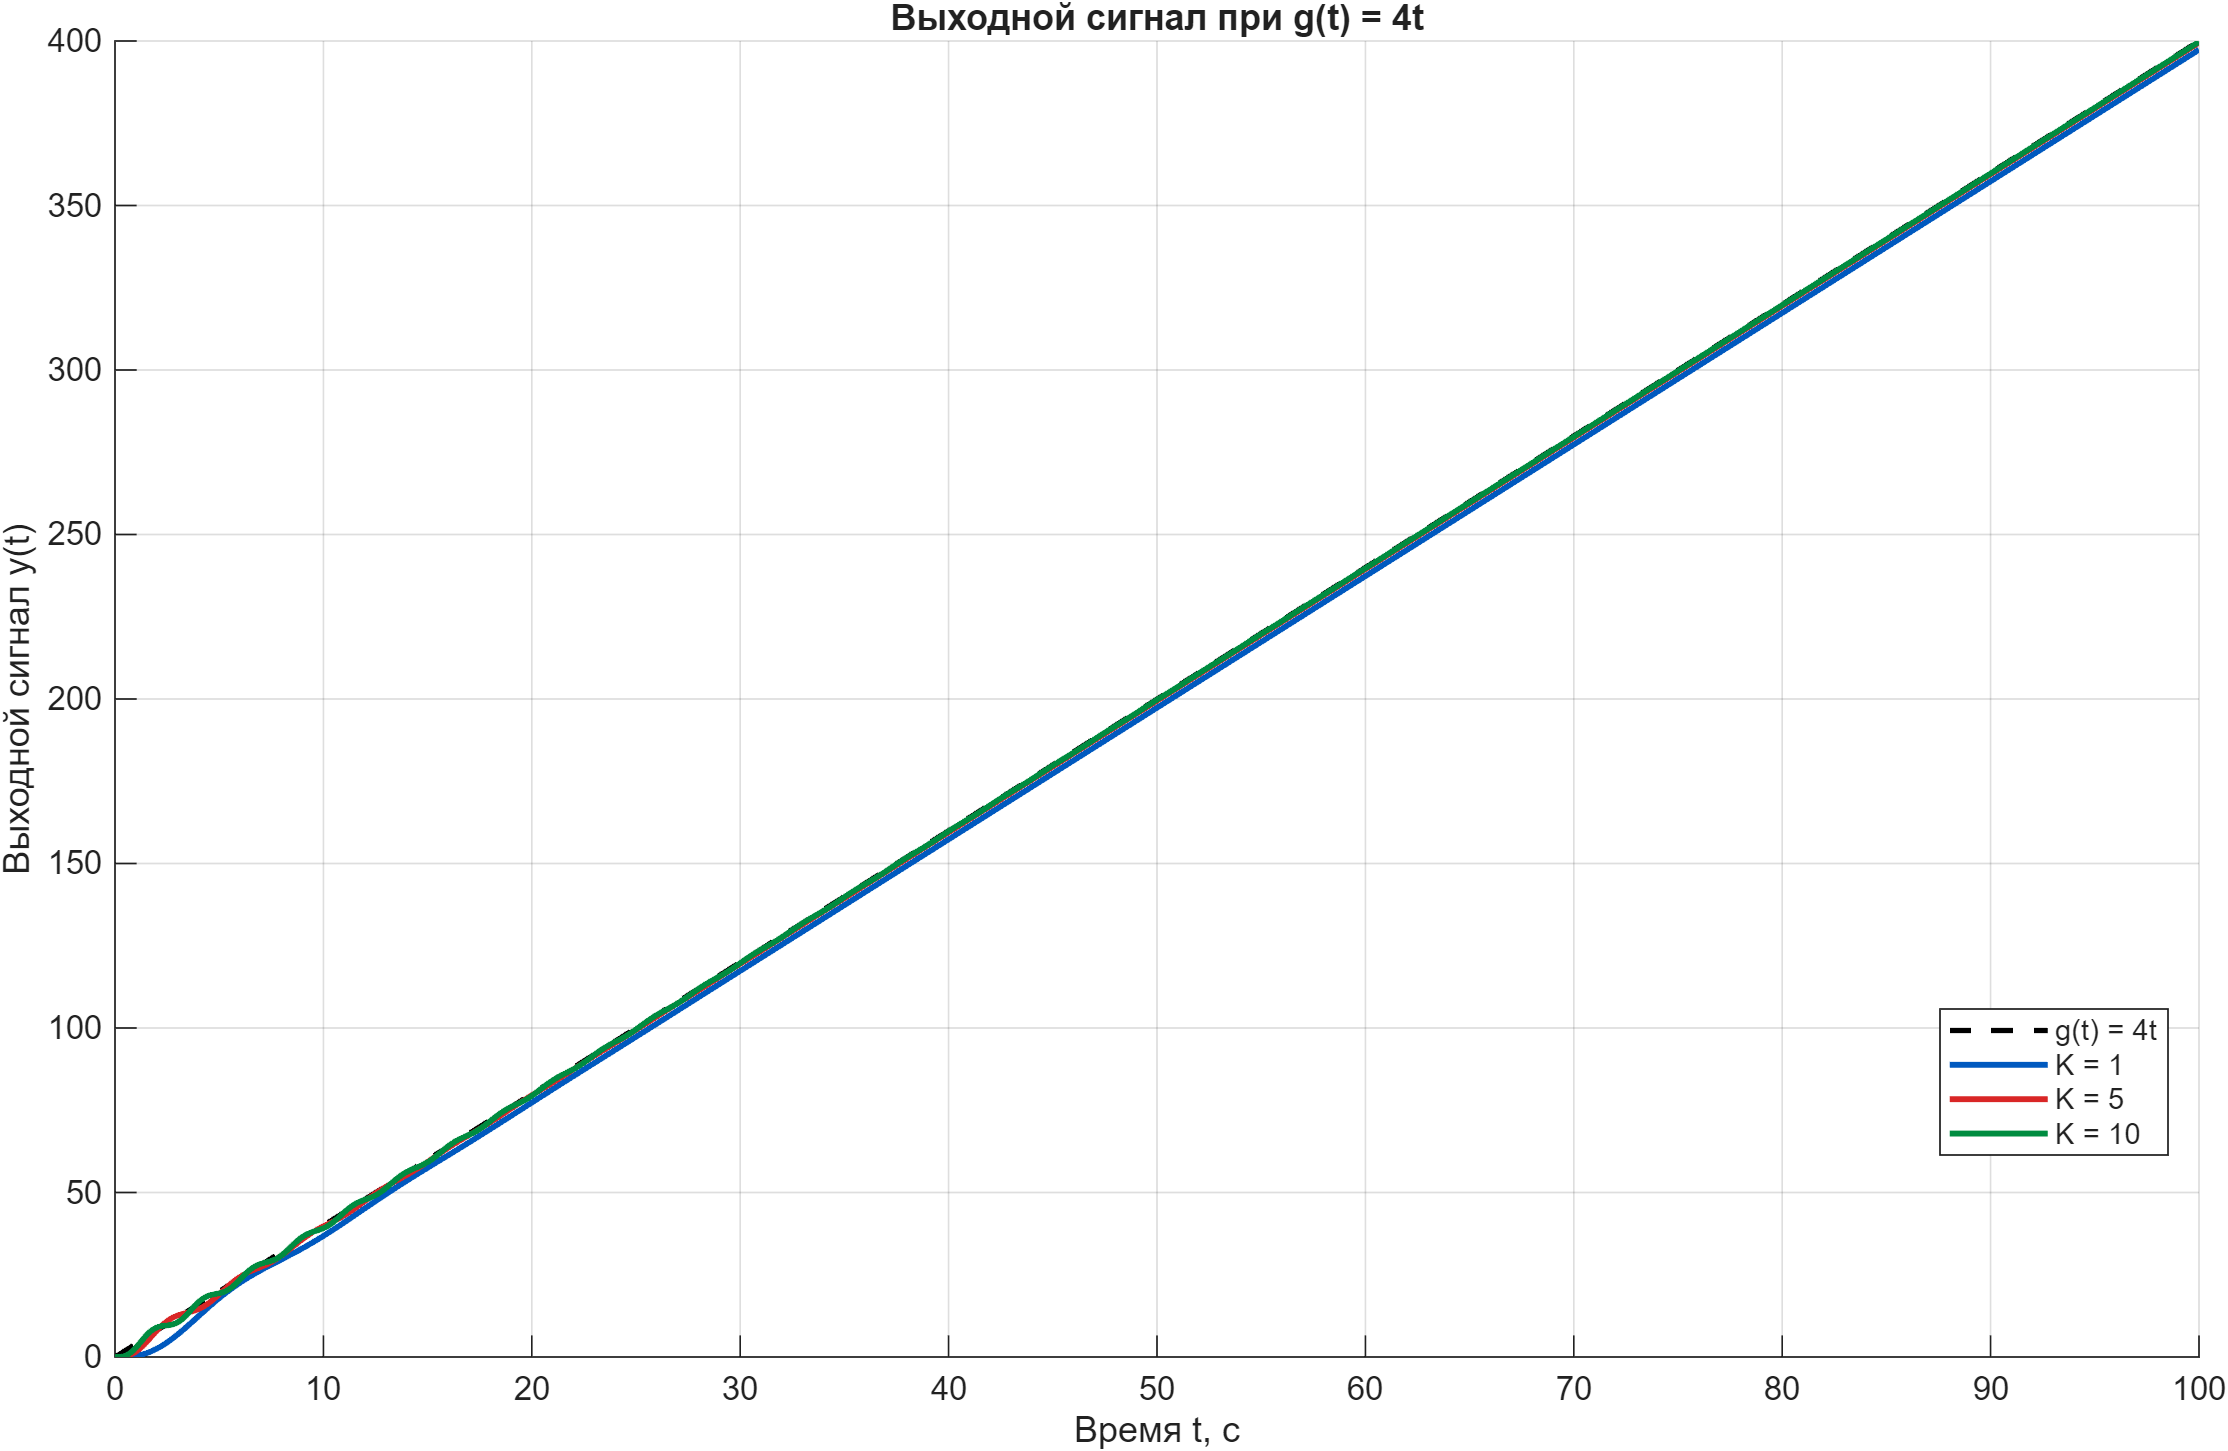
\includegraphics[width=0.85\textwidth]{res2/Lab5_Task2_Figure3.png}
    \caption{Переходные процессы выходного сигнала
    при $g(t)=4t$}
    \label{fig:task2_y_ramp}
\end{figure}

% -----------------------------------------------------------
% ГРАФИК 4 - e(t), g(t) = 4t
% -----------------------------------------------------------
\begin{figure}[H]
    \centering
    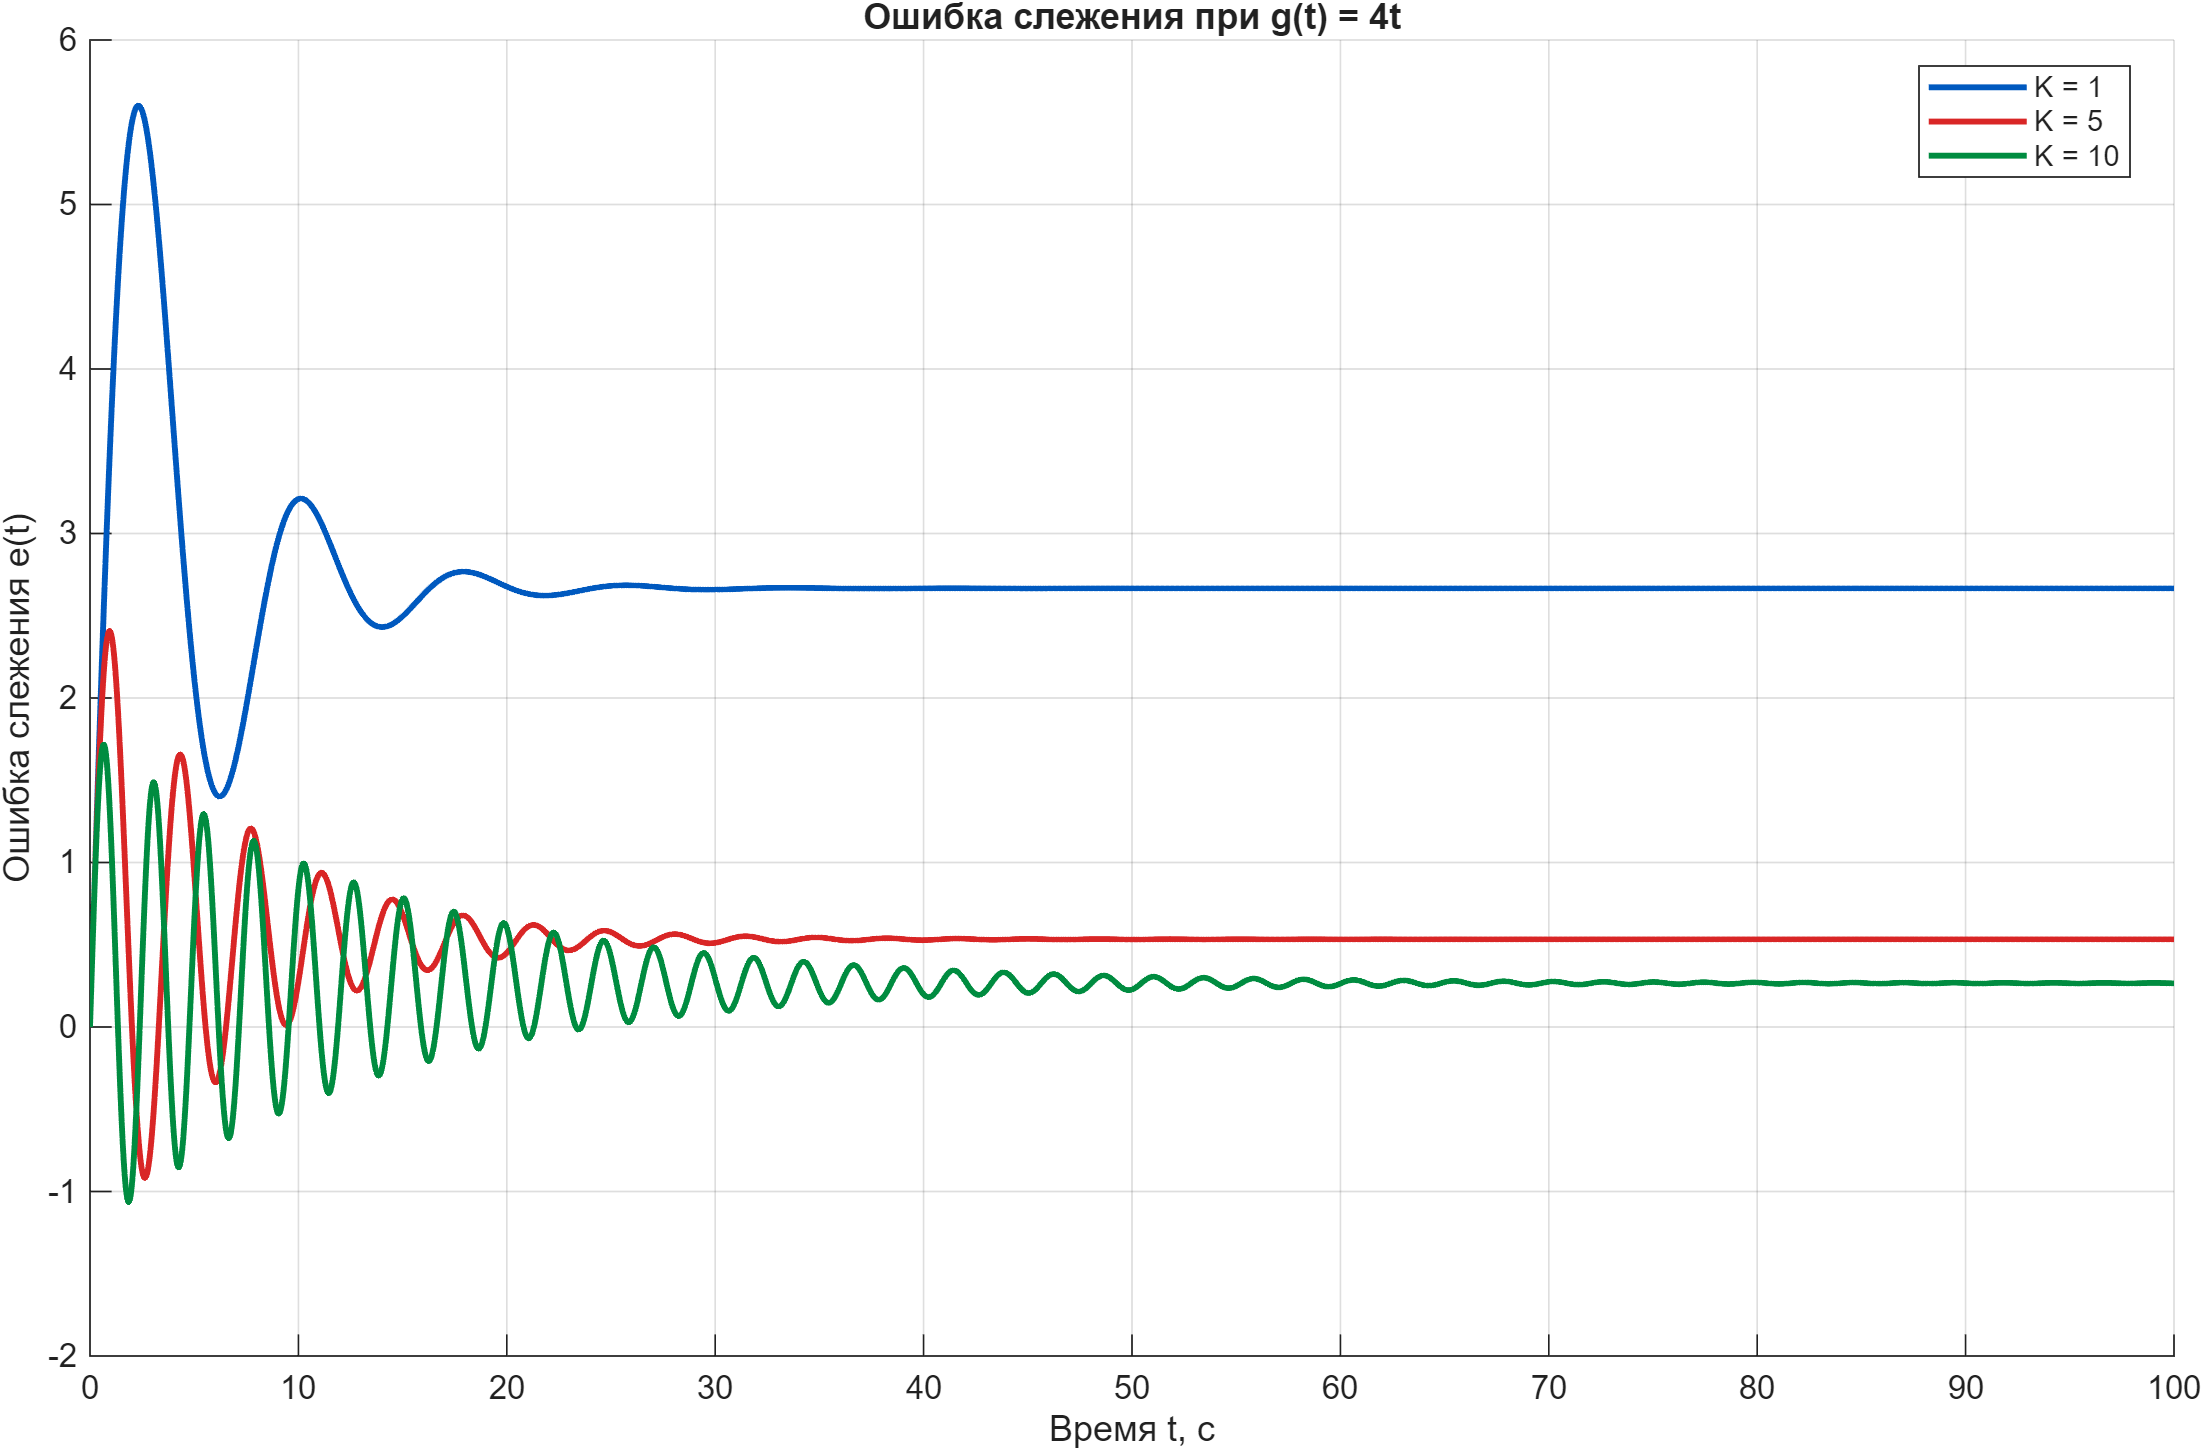
\includegraphics[width=0.85\textwidth]{res2/Lab5_Task2_Figure4.png}
    \caption{Переходные процессы ошибки слежения
    при $g(t)=4t$}
    \label{fig:task2_e_ramp}
\end{figure}

Система с первым порядком астатизма
обеспечивает конечную установившуюся ошибку
при линейно возрастающем задающем воздействии.

При увеличении коэффициента усиления $K$
установившаяся ошибка уменьшается.


\subsection{Исследование при квадратично
возрастающем задающем воздействии}

Рассмотрим задающее воздействие:
\[
    g(t)=0.2t^2.
\]

Его изображение по Лапласу:
\[
    G(s)=\frac{0.4}{s^3}.
\]

Изображение ошибки слежения:
\[
    E(s)=
    \frac{0.1s^3+2.2s^2+s}
    {0.1s^3+2.2s^2+s+1.5K}
    \cdot\frac{0.4}{s^3}.
\]

Для определения установившейся составляющей
ошибки разложим передаточную функцию по ошибке
в ряд Тейлора в окрестности $s=0$:
\[
    W_{g\to e}(s)
    =c_0+c_1s+\frac{c_2}{2}s^2+O(s^3).
\]

Коэффициенты ошибок:
\[
    c_0=0,
    \qquad
    c_1=\frac{1}{1.5K},
\]
\[
    c_2=
    2\left(
    \frac{2.2}{1.5K}
    -\frac{1}{(1.5K)^2}
    \right).
\]

Установившаяся составляющая ошибки:
\[
    e_y(t)=
    c_0g(t)+c_1\dot{g}(t)
    +\frac{c_2}{2}\ddot{g}(t).
\]

Поскольку:
\[
    \dot{g}(t)=0.4t,
    \qquad \ddot{g}(t)=0.4,
\]

получим:
\begin{equation}
    \boxed{
    e_y(t)=
    \frac{0.4}{1.5K}t+
    0.4\left(
    \frac{2.2}{1.5K}
    -\frac{1}{(1.5K)^2}
    \right)
    }.
\end{equation}

Для различных значений коэффициента усиления:
\[
\begin{aligned}
    K=1:\quad
    e_y(t)&\approx0.2667t+0.4089,\\
    K=5:\quad
    e_y(t)&\approx0.05333t+0.1102,\\
    K=10:\quad
    e_y(t)&\approx0.02667t+0.05689.
\end{aligned}
\]

Таким образом, при квадратично возрастающем
задающем воздействии ошибка слежения
неограниченно возрастает.

Для сравнения переходных процессов
проводится моделирование системы при
трёх значениях коэффициента усиления.

% -----------------------------------------------------------
% ГРАФИК 5 - y(t), g(t) = 0.2t^2
% -----------------------------------------------------------
\begin{figure}[H]
    \centering
    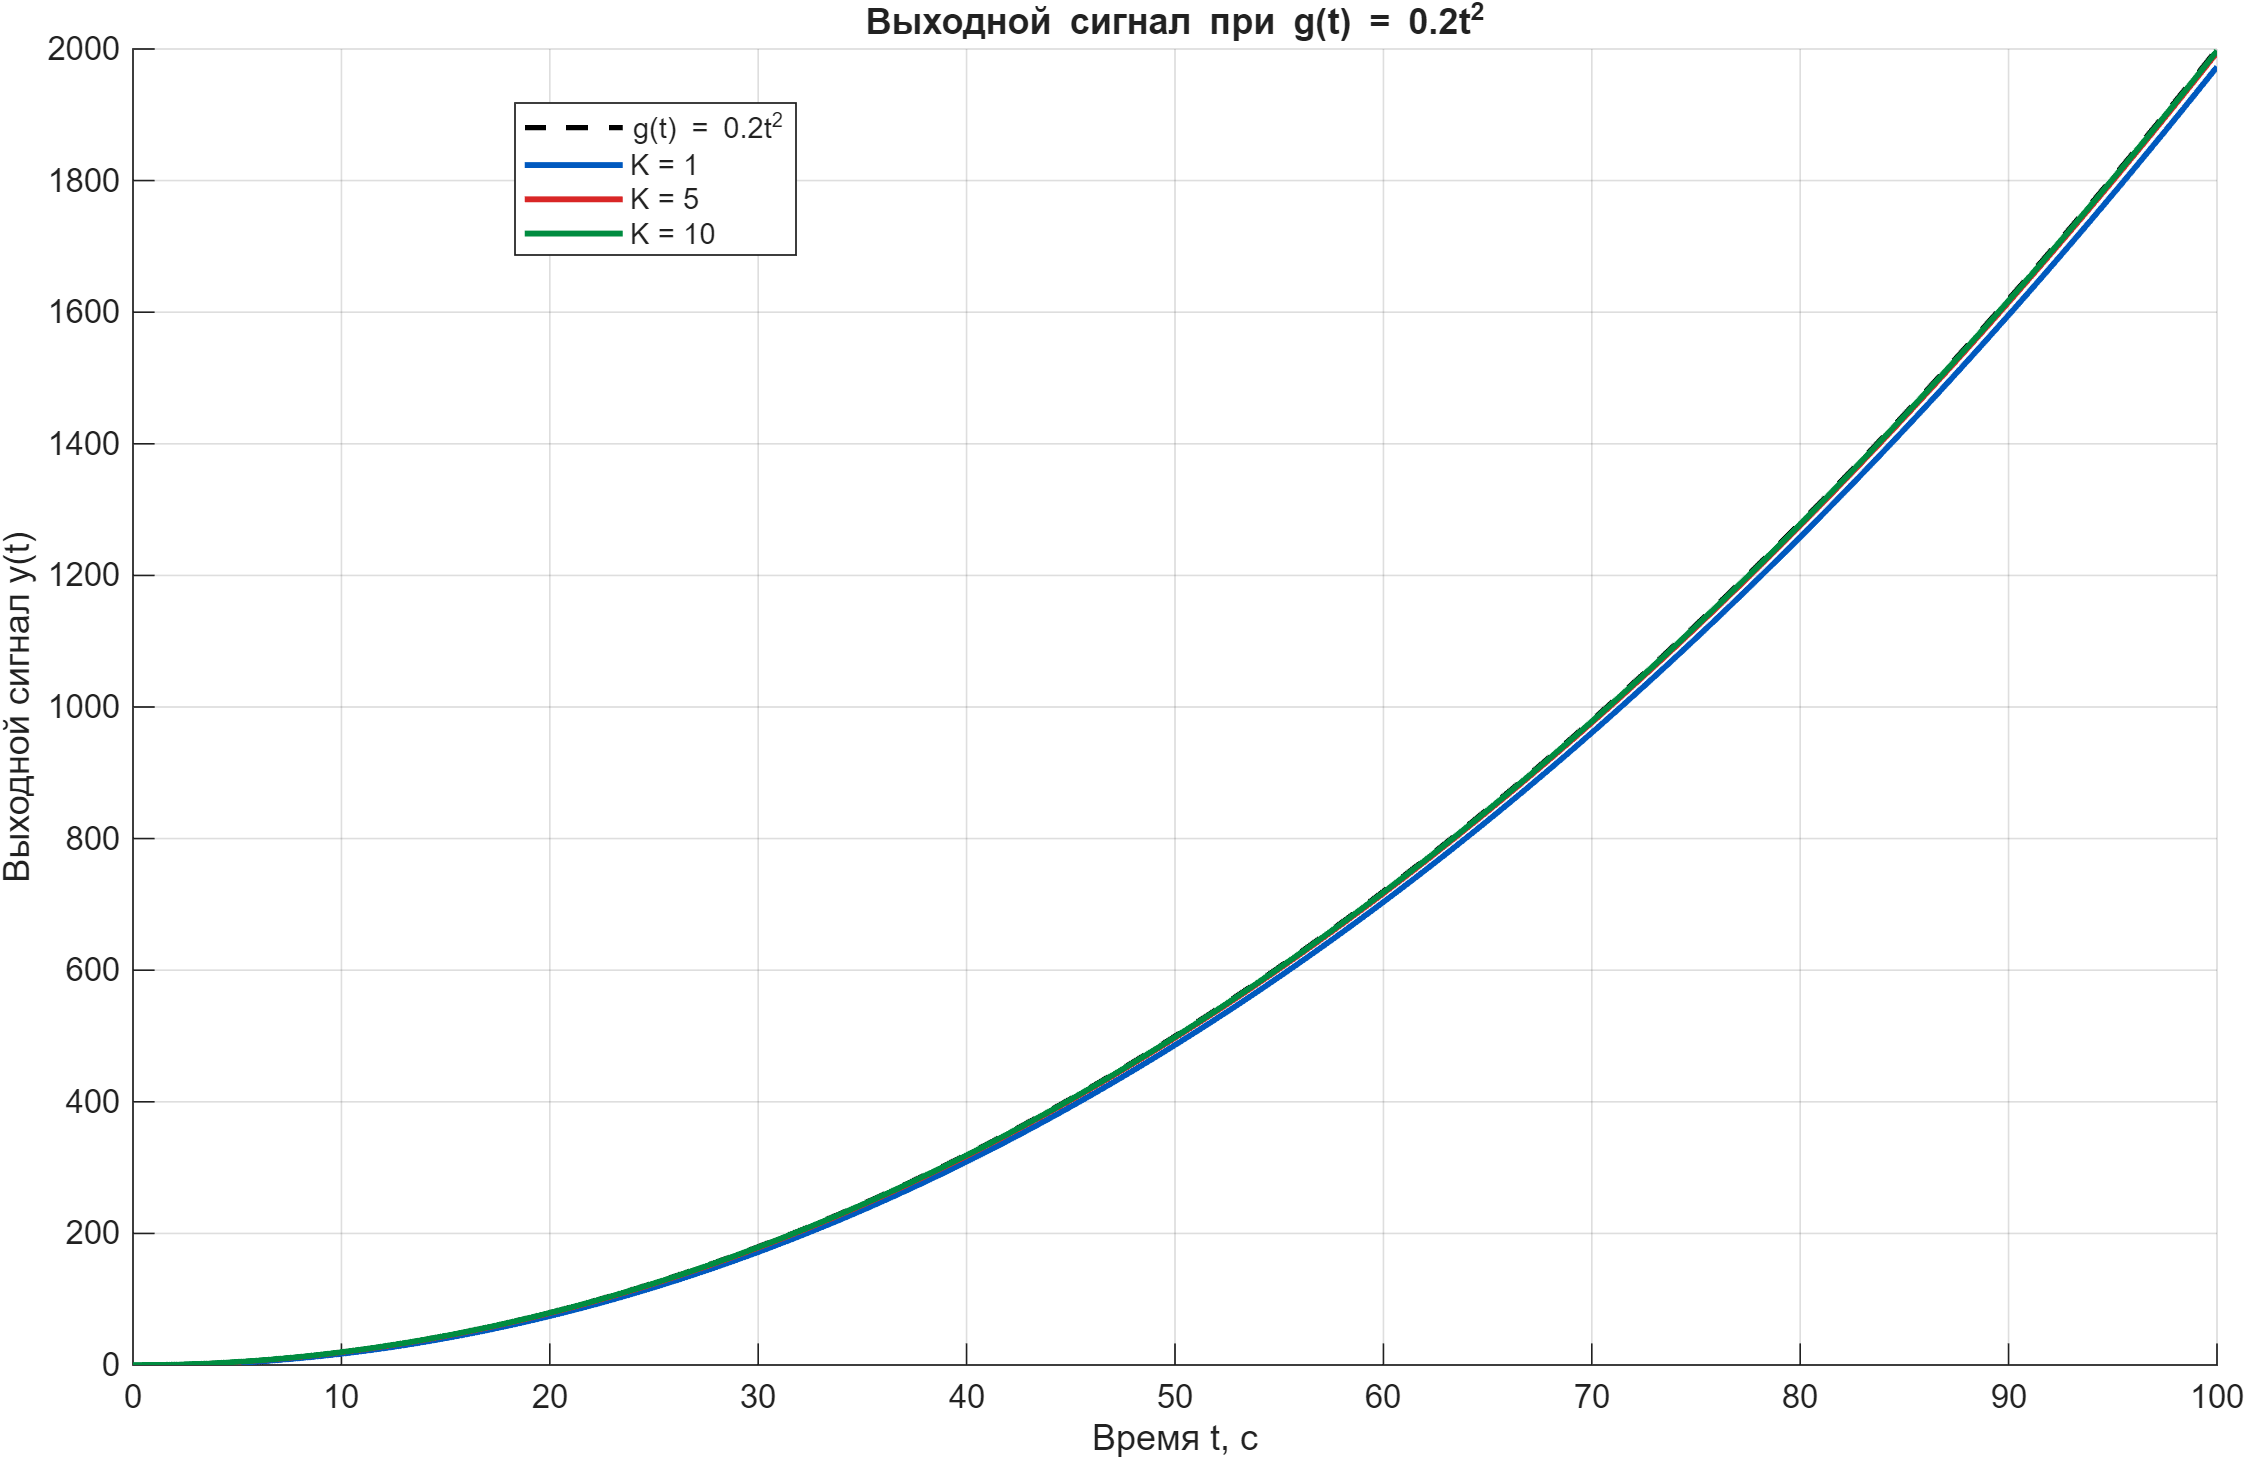
\includegraphics[width=0.85\textwidth]{res2/Lab5_Task2_Figure5.png}
    \caption{Переходные процессы выходного сигнала
    при $g(t)=0.2t^2$}
    \label{fig:task2_y_quadratic}
\end{figure}

% -----------------------------------------------------------
% ГРАФИК 6 - e(t), g(t) = 0.2t^2
% -----------------------------------------------------------
\begin{figure}[H]
    \centering
    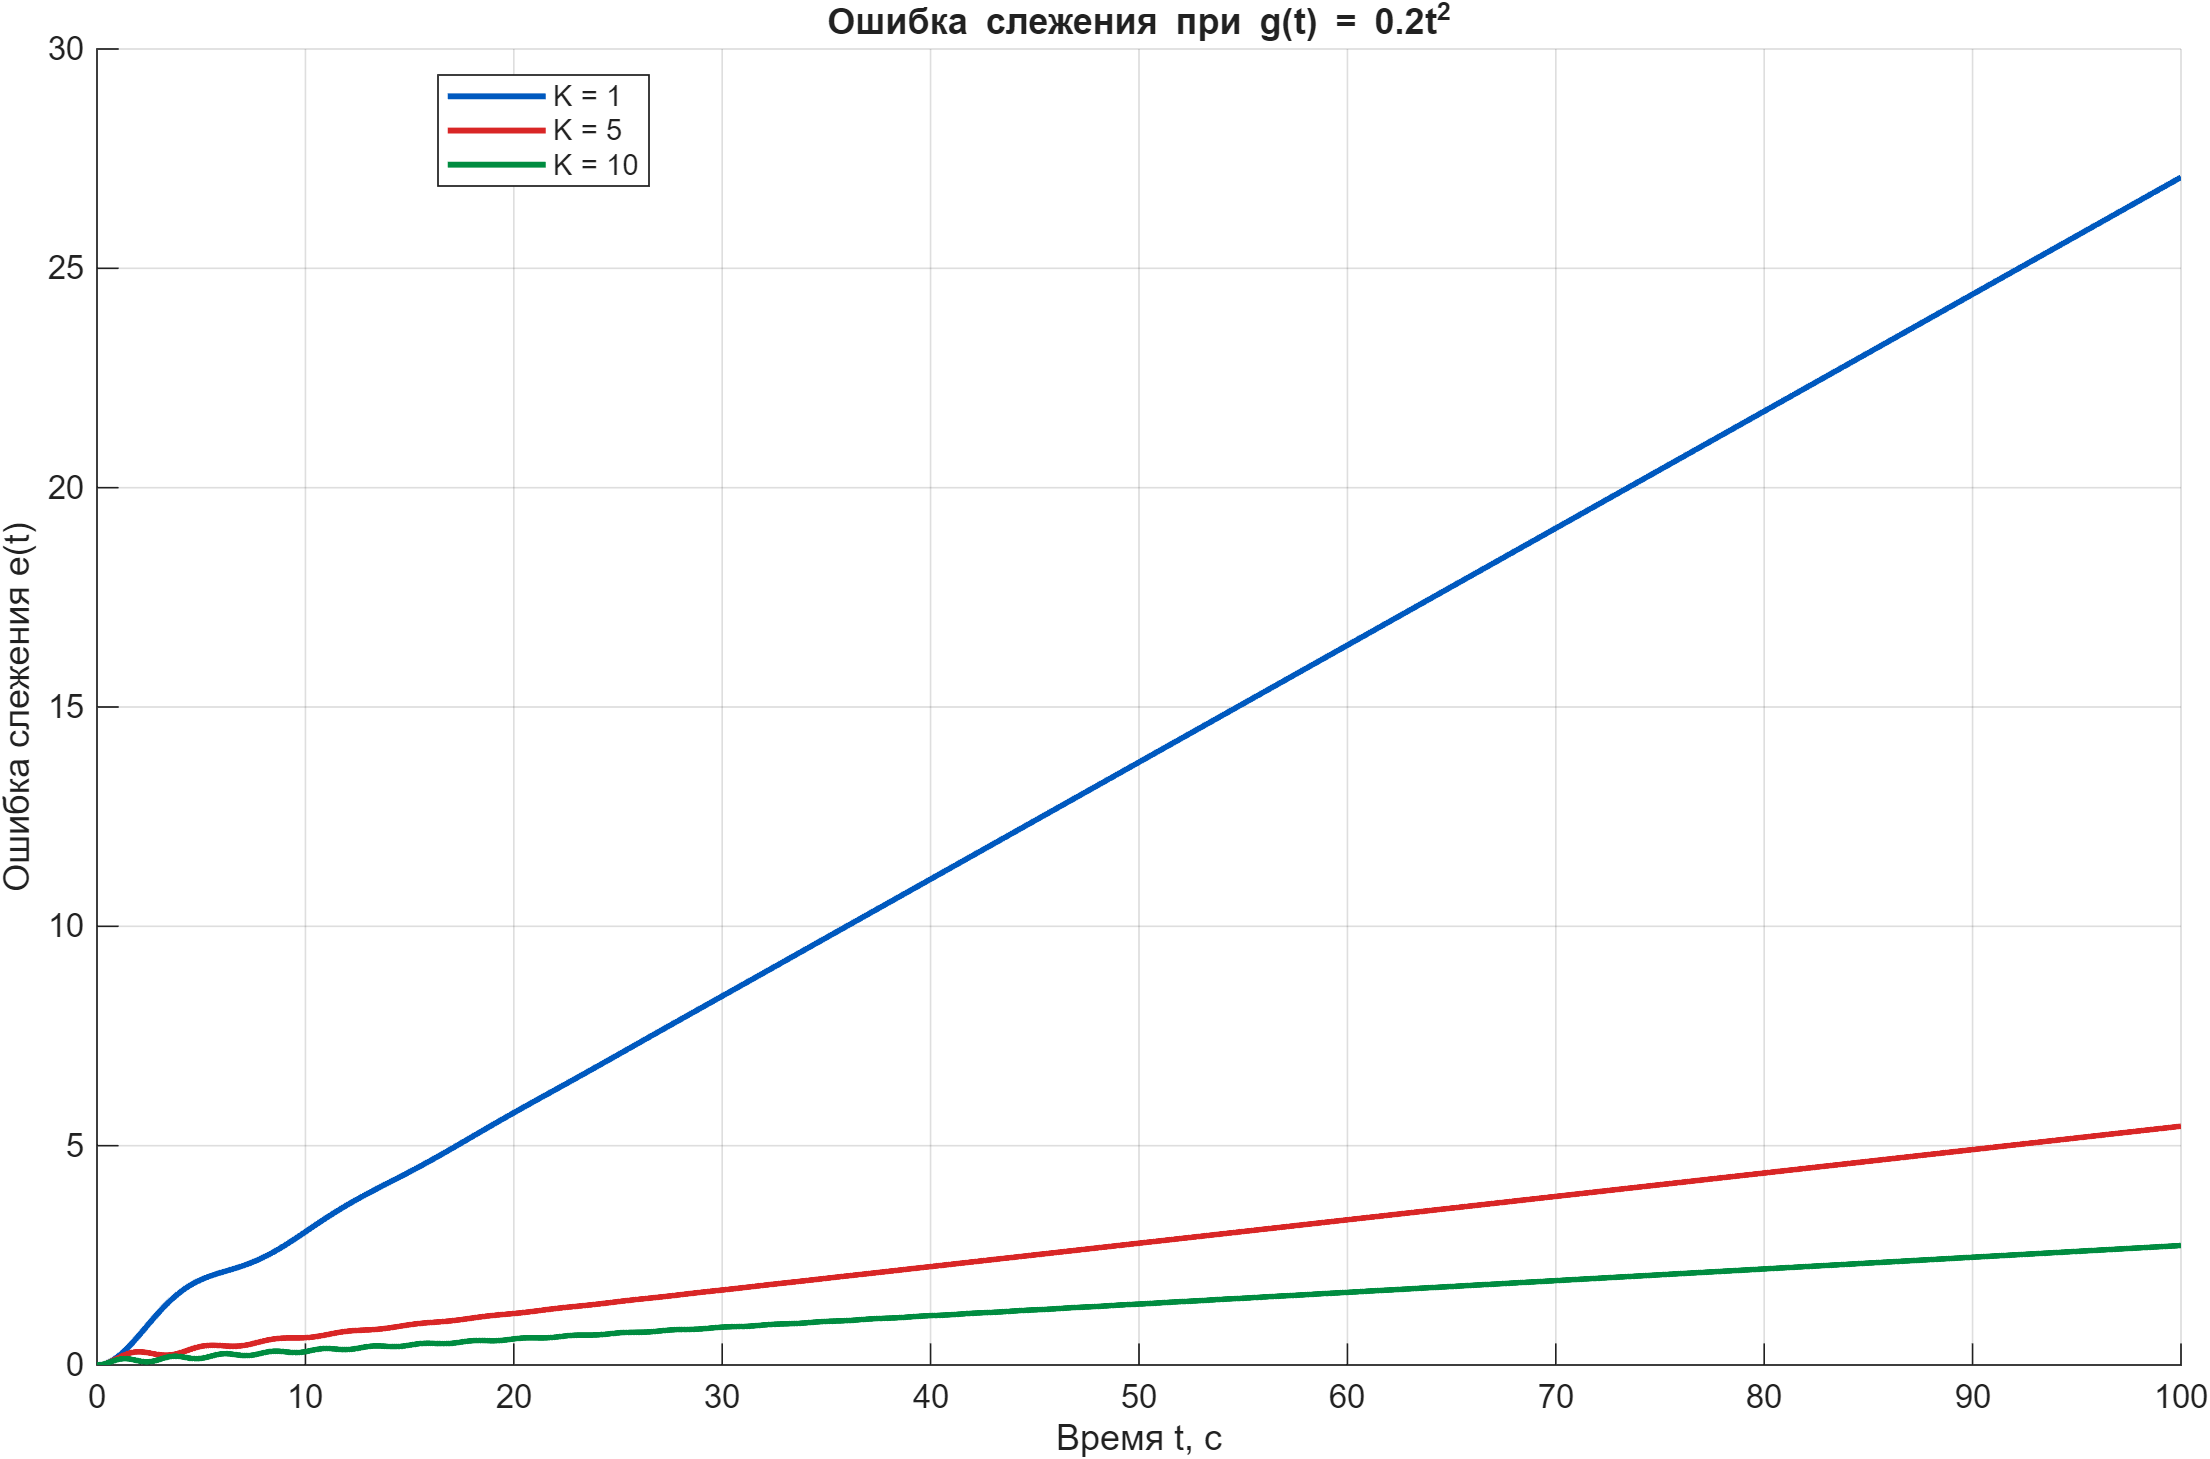
\includegraphics[width=0.85\textwidth]{res2/Lab5_Task2_Figure6.png}
    \caption{Переходные процессы ошибки слежения
    при $g(t)=0.2t^2$}
    \label{fig:task2_e_quadratic}
\end{figure}

Увеличение коэффициента усиления $K$
уменьшает скорость роста ошибки слежения.
Однако интегральный регулятор не обеспечивает
ограниченную ошибку при квадратично
возрастающем задающем воздействии.


\subsection{Вывод по заданию 2}

В ходе выполнения задания исследованы
точностные свойства системы с интегральным
регулятором при различных задающих воздействиях.

При постоянном задающем воздействии
установившаяся ошибка равна нулю
для всех рассматриваемых значений $K$.

При линейно возрастающем воздействии
установившаяся ошибка имеет конечное
ненулевое значение и уменьшается
с увеличением коэффициента усиления.

При квадратично возрастающем воздействии
ошибка слежения неограниченно возрастает.

Таким образом, интегральный регулятор
обеспечивает первый порядок астатизма
и повышает точность слежения по сравнению
с пропорциональным регулятором.




% ===========================================================
% ЗАДАНИЕ 3. ПРОПОРЦИОНАЛЬНО-ИНТЕГРАЛЬНЫЙ РЕГУЛЯТОР
% ===========================================================

\newpage
\section{Задание 3. Пропорционально-интегральный регулятор}

\subsection{Исходные данные}

В соответствии с вариантом 3 передаточная функция
объекта управления имеет вид:
\[
    W(s)=\frac{1.5}{0.1s^2+2.2s+1}.
\]

В системе используется пропорционально-интегральный
регулятор с передаточной функцией:
\begin{equation}
    \boxed{
    H(s)=K_{\text{п}}+\frac{K_{\text{и}}}{s}
    }.
\end{equation}

Рассматривается замкнутая система управления
с единичной отрицательной обратной связью.

Задающее воздействие изменяется
с постоянной скоростью:
\[
    g(t)=Vt=4t.
\]

В соответствии с таблицей параметров регулятора
необходимо провести девять экспериментов
при различных значениях коэффициентов
$K_{\text{п}}$ и $K_{\text{и}}$.

Параметры регулятора представлены
в таблице~\ref{tab:task3_parameters}.

\begin{table}[H]
    \centering
    \caption{Параметры ПИ-регулятора}
    \label{tab:task3_parameters}

    \setlength{\tabcolsep}{30pt}

    \begin{tabular}{ccc}
        \toprule
        Номер эксперимента &
        $K_{\text{п}}$ & $K_{\text{и}}$ \\
        \midrule
        1 & 1  & 1  \\
        2 & 5  & 1  \\
        3 & 10 & 1  \\
        4 & 1  & 5  \\
        5 & 5  & 5  \\
        6 & 10 & 5  \\
        7 & 1  & 10 \\
        8 & 5  & 10 \\
        9 & 10 & 10 \\
        \bottomrule
    \end{tabular}
\end{table}

Структурная схема исследуемой системы
представлена на рисунке~\ref{fig:task3_schema}.

% -----------------------------------------------------------
% СТРУКТУРНАЯ СХЕМА
% -----------------------------------------------------------
\begin{figure}[H]
    \centering
    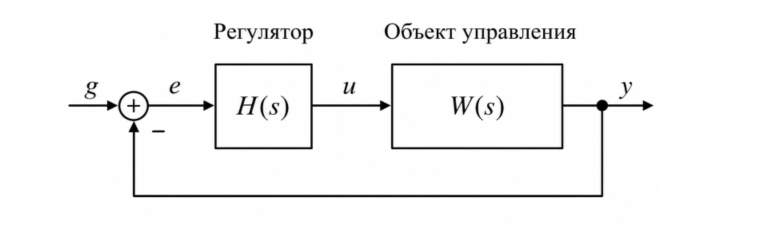
\includegraphics[width=0.85\textwidth]{schema_task1.png}
    \caption{Структурная схема замкнутой системы с ПИ-регулятором}
    \label{fig:task3_schema}
\end{figure}


\subsection{Передаточные функции системы}

Передаточная функция ПИ-регулятора может
быть представлена в виде:
\[
    H(s)=
    \frac{K_{\text{п}}s+K_{\text{и}}}{s}.
\]

Передаточная функция разомкнутой системы:
\[
    L(s)=H(s)W(s).
\]

После подстановки:
\[
    L(s)=
    \frac{1.5(K_{\text{п}}s+K_{\text{и}})}
    {s(0.1s^2+2.2s+1)}.
\]

Передаточная функция замкнутой системы
по задающему воздействию определяется
выражением:
\[
    T(s)=\frac{L(s)}{1+L(s)}.
\]

Следовательно:
\begin{equation}
    \boxed{
    T(s)=
    \frac{1.5(K_{\text{п}}s+K_{\text{и}})}
    {0.1s^3+2.2s^2+
    (1+1.5K_{\text{п}})s+1.5K_{\text{и}}}
    }.
\end{equation}

Передаточная функция замкнутой системы
по ошибке:
\[
    W_{g\to e}(s)=\frac{1}{1+L(s)}.
\]

Подставляя выражение для $L(s)$, получим:
\begin{equation}
    \boxed{
    W_{g\to e}(s)=
    \frac{0.1s^3+2.2s^2+s}
    {0.1s^3+2.2s^2+
    (1+1.5K_{\text{п}})s+1.5K_{\text{и}}}
    }.
\end{equation}

Характеристический полином замкнутой системы:
\[
    D(s)=0.1s^3+2.2s^2+
    (1+1.5K_{\text{п}})s+1.5K_{\text{и}}.
\]

Для проверки устойчивости воспользуемся
критерием Гурвица.

Для полинома третьего порядка при положительных
коэффициентах должно выполняться условие:
\[
    2.2(1+1.5K_{\text{п}})
    >0.15K_{\text{и}}.
\]

Для всех девяти рассматриваемых сочетаний
коэффициентов данное условие выполняется.

Следовательно, замкнутая система
асимптотически устойчива во всех экспериментах.

Наличие интегральной составляющей регулятора
обеспечивает первый порядок астатизма системы.


\subsection{Аналитический расчёт
установившейся ошибки}

Рассмотрим линейно возрастающее
задающее воздействие:
\[
    g(t)=4t.
\]

Его изображение по Лапласу:
\[
    G(s)=\frac{4}{s^2}.
\]

Изображение ошибки слежения:
\[
    E(s)=W_{g\to e}(s)G(s).
\]

Подставляя полученную передаточную функцию
по ошибке, получим:
\[
    E(s)=
    \frac{0.1s^3+2.2s^2+s}
    {0.1s^3+2.2s^2+
    (1+1.5K_{\text{п}})s+1.5K_{\text{и}}}
    \cdot\frac{4}{s^2}.
\]

Для определения предельного значения
установившейся ошибки воспользуемся
теоремой о предельном значении:
\[
    \varepsilon=
    \lim_{t\to\infty}e(t)
    =\lim_{s\to0}sE(s).
\]

Тогда:
\[
    \varepsilon=
    \lim_{s\to0}
    \frac{4(0.1s^2+2.2s+1)}
    {0.1s^3+2.2s^2+
    (1+1.5K_{\text{п}})s+1.5K_{\text{и}}}.
\]

В результате получим:
\begin{equation}
    \boxed{
    \varepsilon=\frac{4}{1.5K_{\text{и}}}
    }.
\end{equation}

Из полученного выражения следует, что
установившаяся ошибка зависит только
от интегрального коэффициента $K_{\text{и}}$
и не зависит от пропорционального
коэффициента $K_{\text{п}}$.

При $K_{\text{и}}=1$:
\[
    \varepsilon=\frac{4}{1.5}
    \approx2.6667.
\]

При $K_{\text{и}}=5$:
\[
    \varepsilon=\frac{4}{7.5}
    \approx0.5333.
\]

При $K_{\text{и}}=10$:
\[
    \varepsilon=\frac{4}{15}
    \approx0.2667.
\]

Результаты аналитического расчёта
для всех экспериментов представлены
в таблице~\ref{tab:task3_errors}.

\begin{table}[H]
    \centering
    \caption{Аналитические значения установившейся ошибки}
    \label{tab:task3_errors}

    \setlength{\tabcolsep}{25pt}

    \begin{tabular}{cccc}
        \toprule
        Номер & $K_{\text{п}}$ &
        $K_{\text{и}}$ & $\varepsilon$ \\
        \midrule
        1 & 1  & 1  & 2.6667 \\
        2 & 5  & 1  & 2.6667 \\
        3 & 10 & 1  & 2.6667 \\
        4 & 1  & 5  & 0.5333 \\
        5 & 5  & 5  & 0.5333 \\
        6 & 10 & 5  & 0.5333 \\
        7 & 1  & 10 & 0.2667 \\
        8 & 5  & 10 & 0.2667 \\
        9 & 10 & 10 & 0.2667 \\
        \bottomrule
    \end{tabular}
\end{table}


\subsection{Моделирование при $K_{\text{и}}=1$}

Для первого набора экспериментов принимаем:
\[
    K_{\text{и}}=1,\qquad
    K_{\text{п}}\in\{1,5,10\}.
\]

Аналитически полученная установившаяся ошибка:
\[
    \varepsilon\approx2.6667.
\]

Проводится моделирование переходных процессов
выходного сигнала и ошибки слежения
при различных значениях $K_{\text{п}}$.

% -----------------------------------------------------------
% ГРАФИК 1 - y(t), Kи = 1
% -----------------------------------------------------------
\begin{figure}[H]
    \centering
    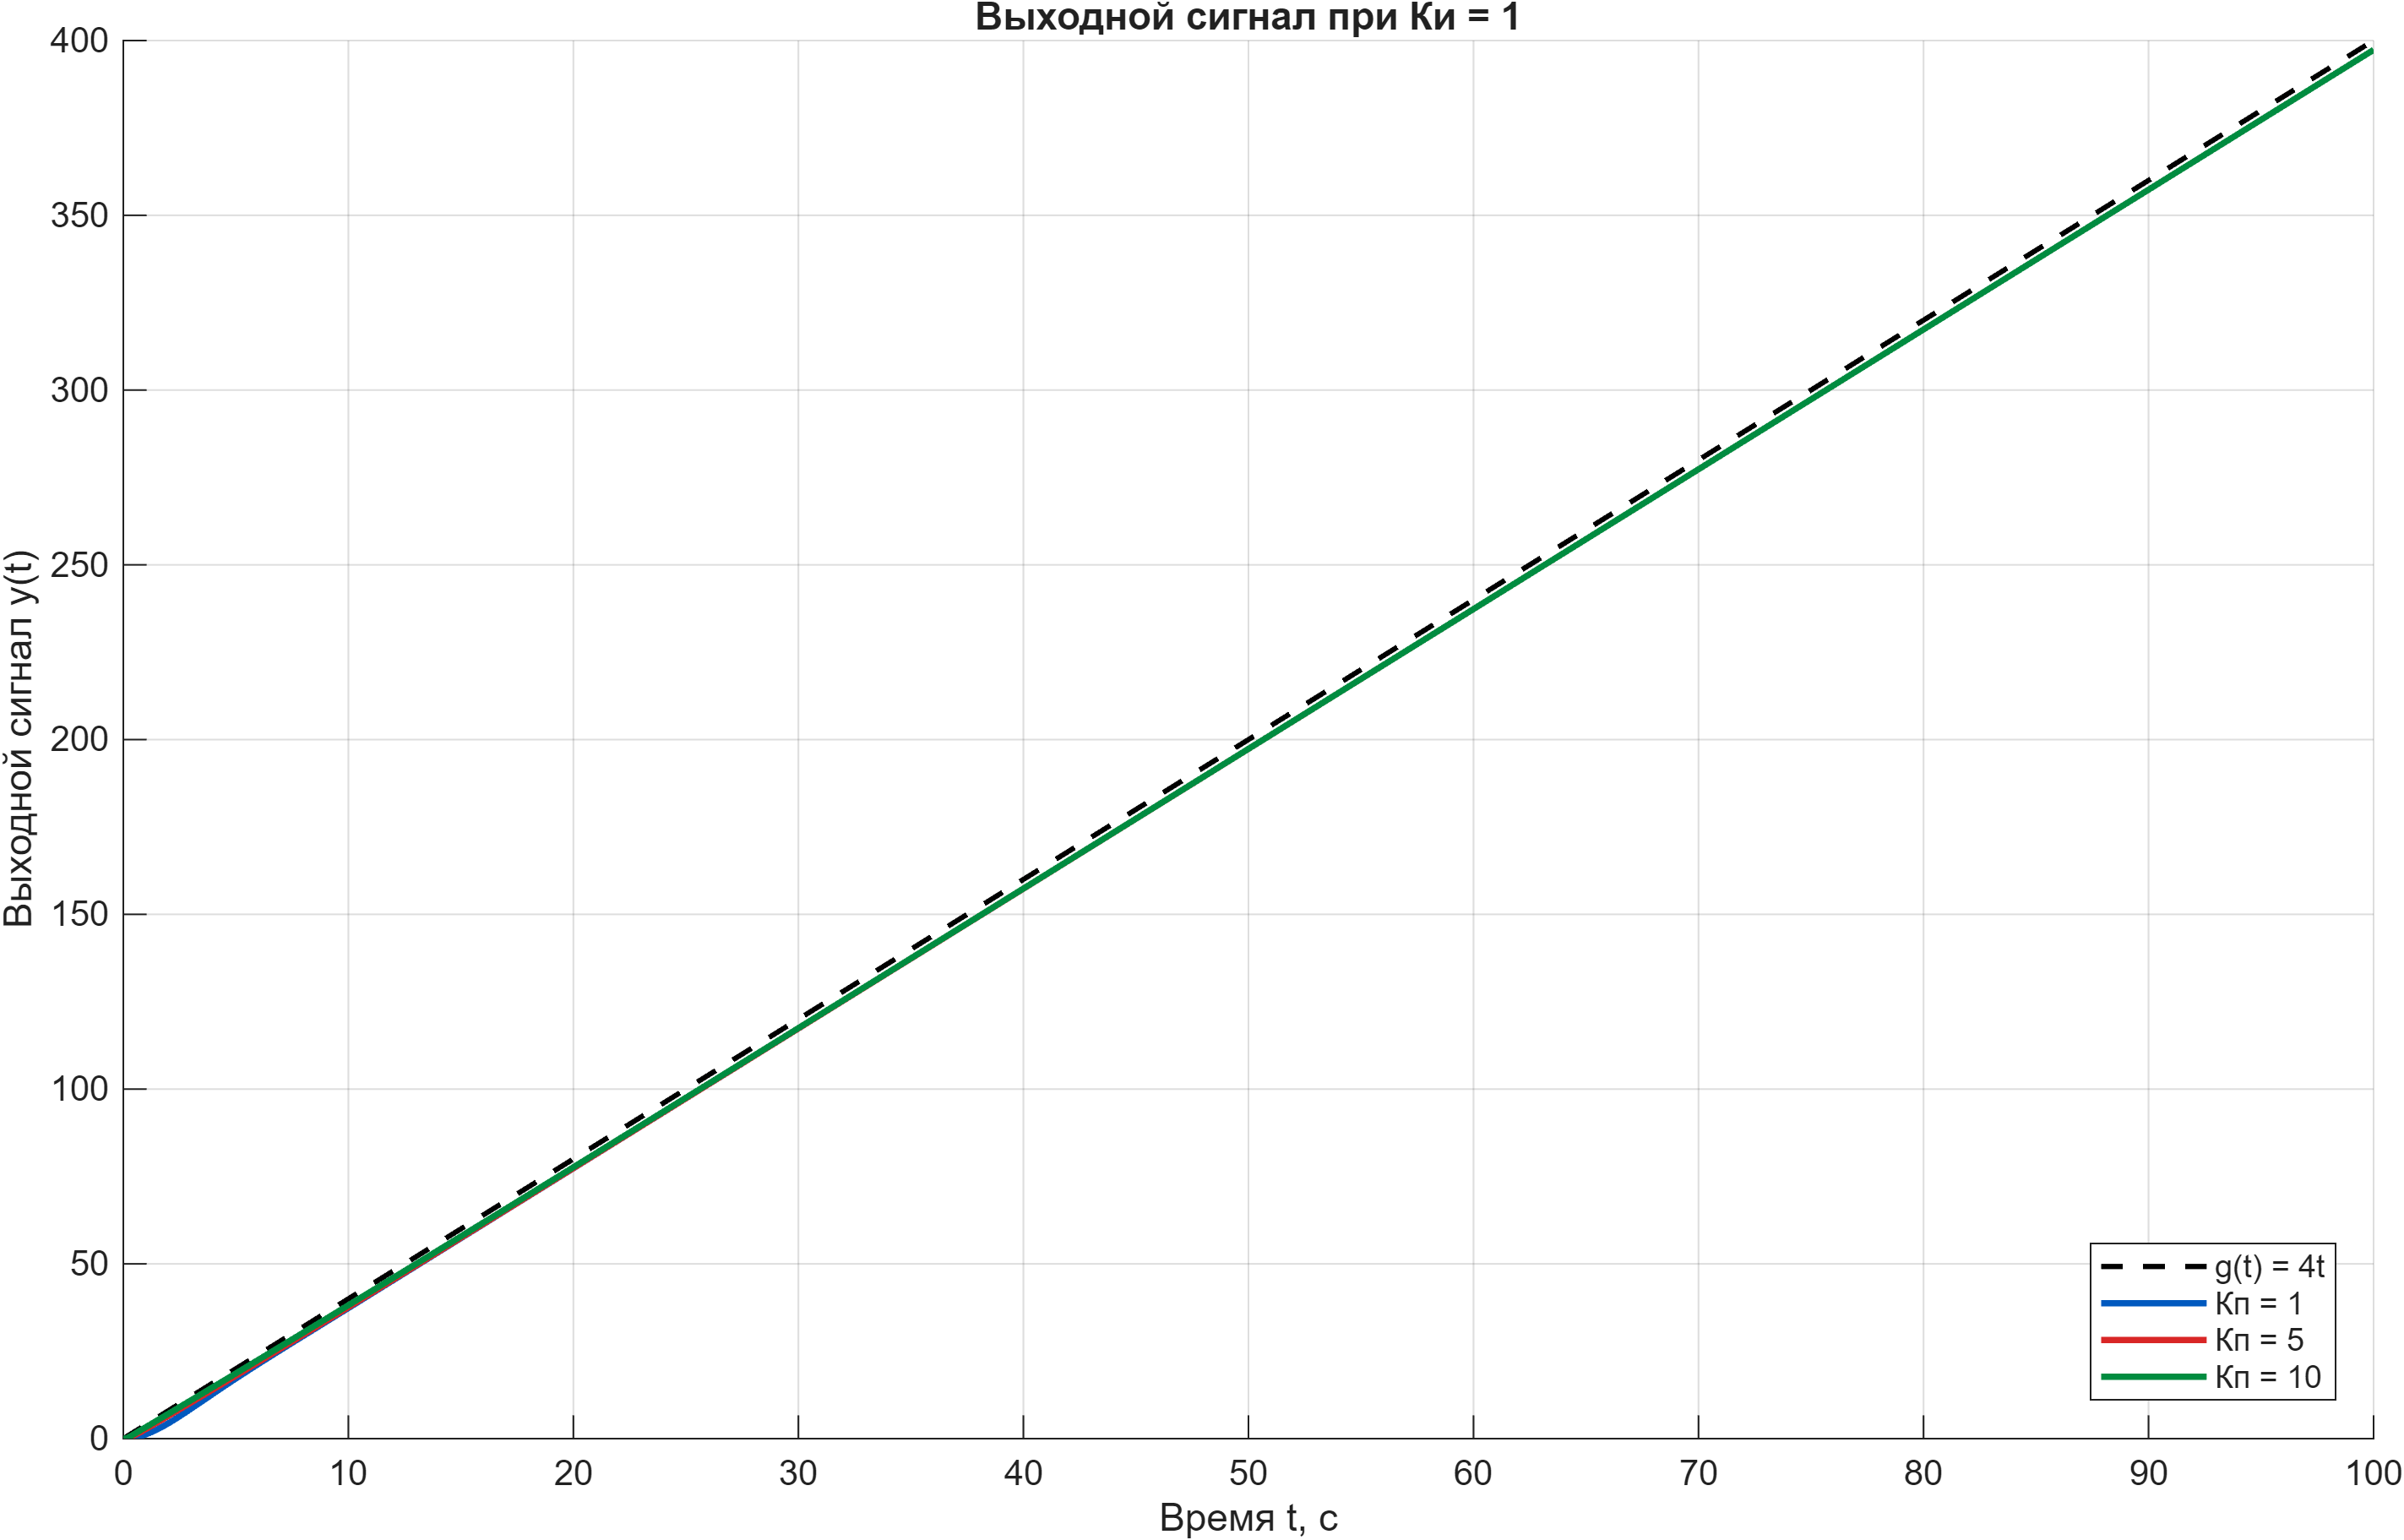
\includegraphics[width=0.85\textwidth]{res3/Lab5_Task3_Figure1.png}
    \caption{Переходные процессы выходного сигнала
    при $K_{\text{и}}=1$}
    \label{fig:task3_y_ki1}
\end{figure}

% -----------------------------------------------------------
% ГРАФИК 2 - e(t), Kи = 1
% -----------------------------------------------------------
\begin{figure}[H]
    \centering
    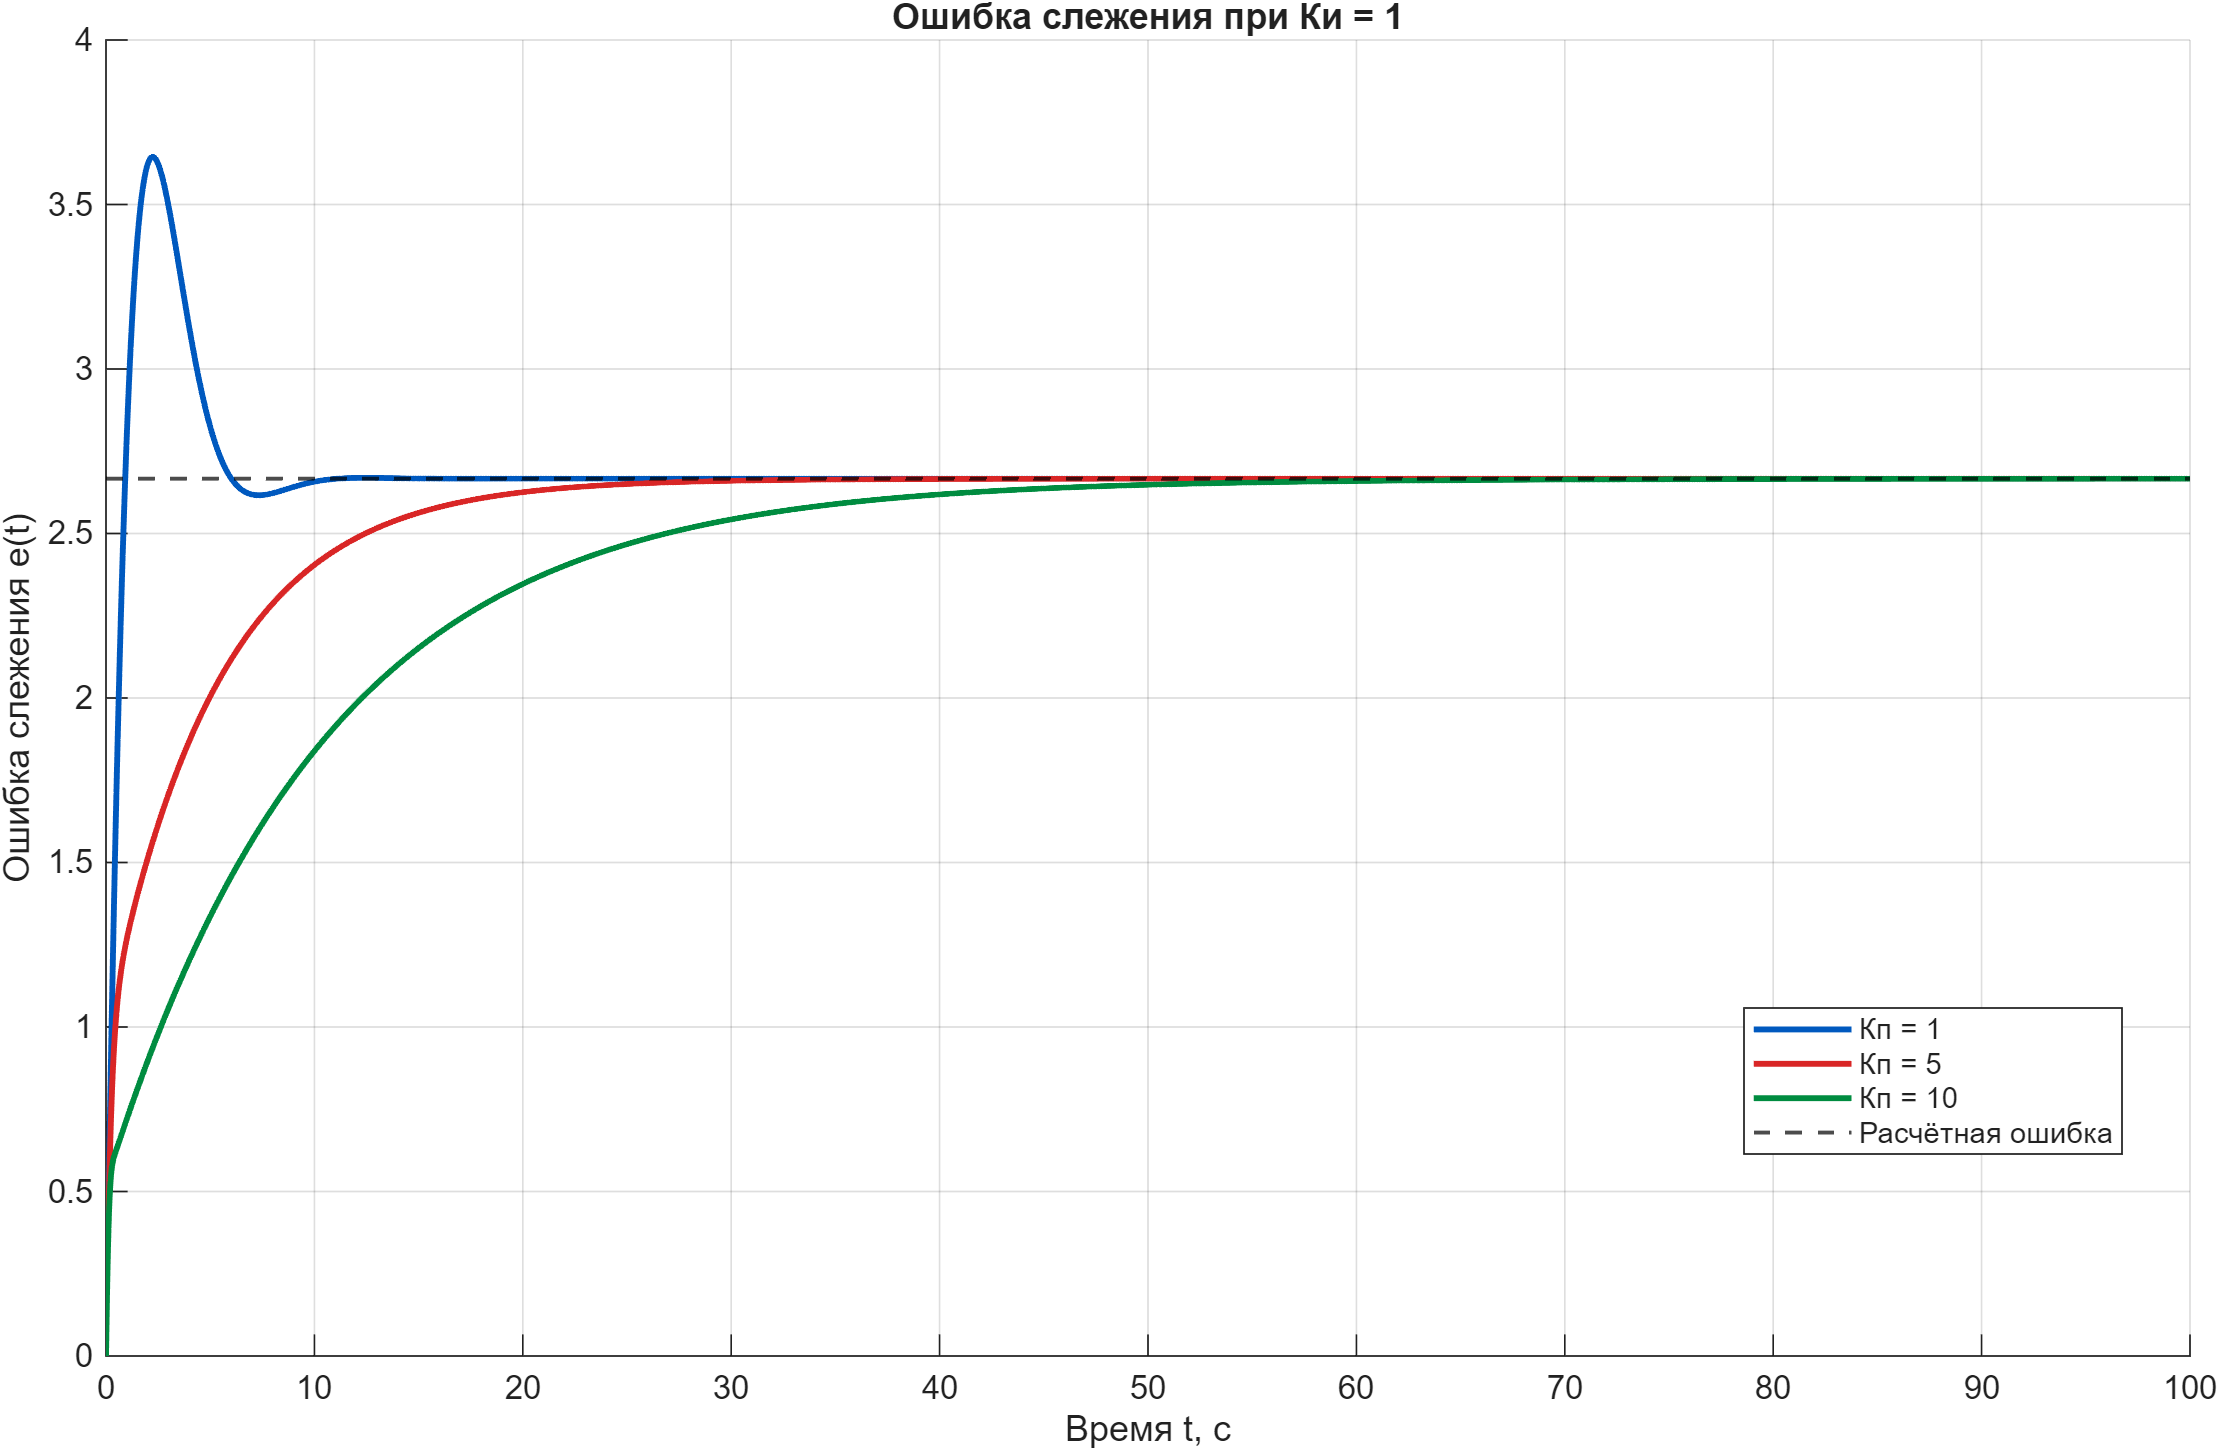
\includegraphics[width=0.85\textwidth]{res3/Lab5_Task3_Figure2.png}
    \caption{Переходные процессы ошибки слежения
    при $K_{\text{и}}=1$}
    \label{fig:task3_e_ki1}
\end{figure}

При фиксированном значении $K_{\text{и}}$
изменение пропорционального коэффициента
влияет на характер переходных процессов,
но не изменяет установившуюся ошибку.


\subsection{Моделирование при $K_{\text{и}}=5$}

Для второго набора экспериментов принимаем:
\[
    K_{\text{и}}=5,\qquad
    K_{\text{п}}\in\{1,5,10\}.
\]

Аналитически полученная установившаяся ошибка:
\[
    \varepsilon\approx0.5333.
\]

Проводится моделирование переходных процессов
при трёх значениях пропорционального коэффициента.

% -----------------------------------------------------------
% ГРАФИК 3 - y(t), Kи = 5
% -----------------------------------------------------------
\begin{figure}[H]
    \centering
    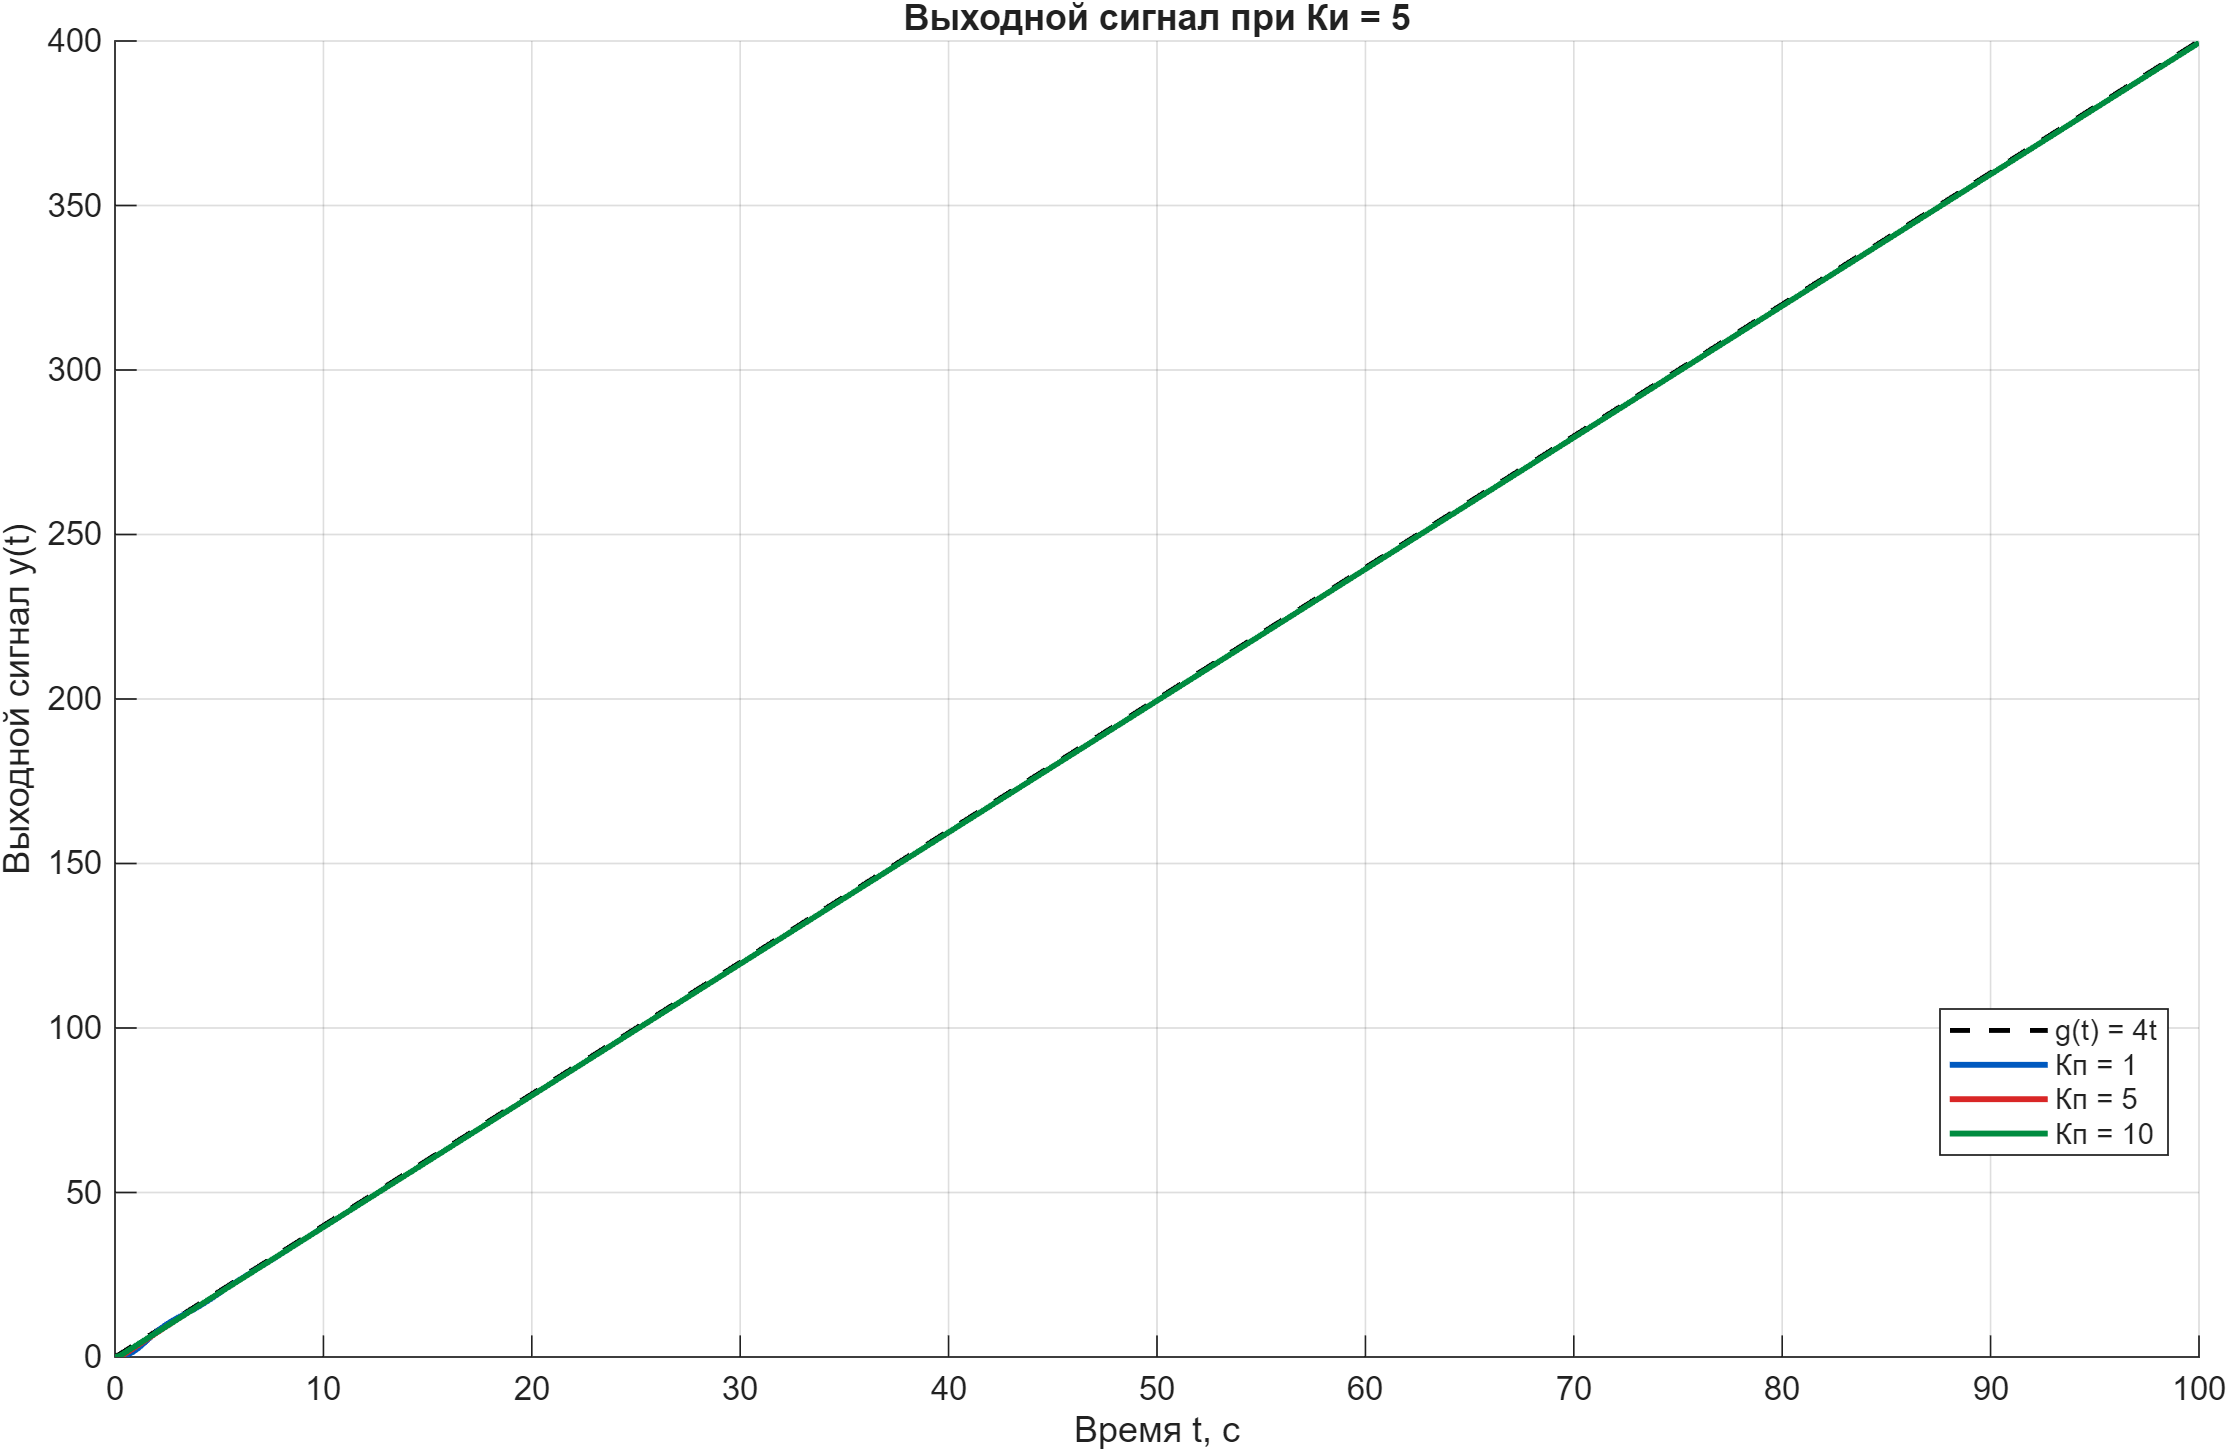
\includegraphics[width=0.85\textwidth]{res3/Lab5_Task3_Figure3.png}
    \caption{Переходные процессы выходного сигнала
    при $K_{\text{и}}=5$}
    \label{fig:task3_y_ki5}
\end{figure}

% -----------------------------------------------------------
% ГРАФИК 4 - e(t), Kи = 5
% -----------------------------------------------------------
\begin{figure}[H]
    \centering
    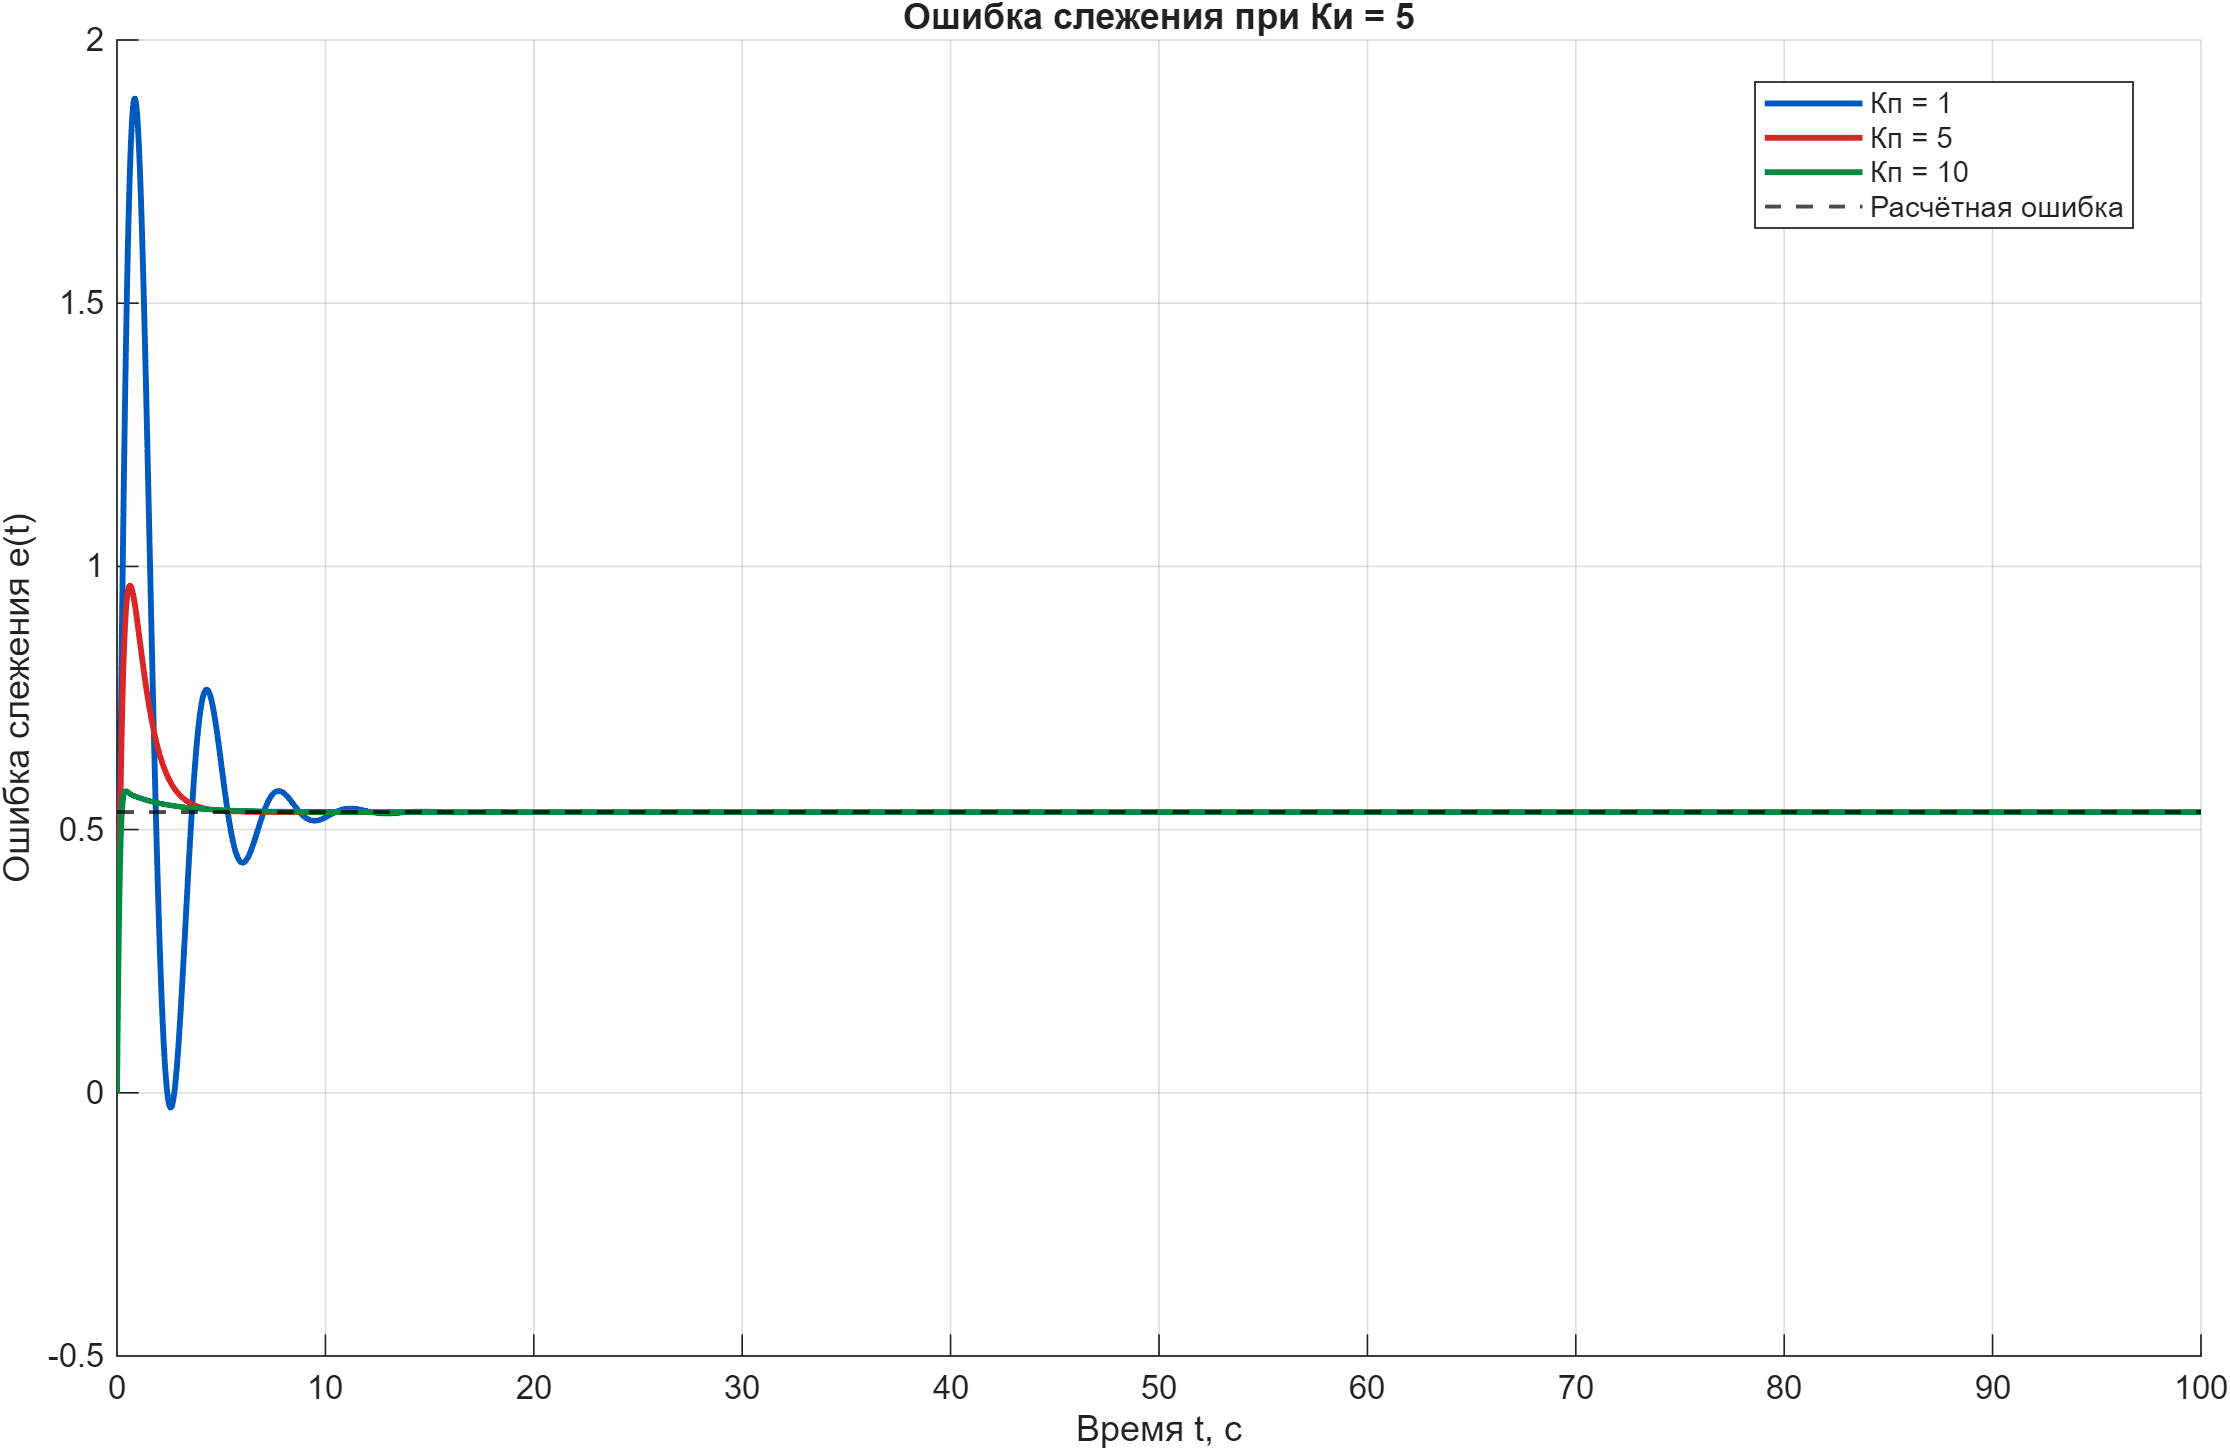
\includegraphics[width=0.85\textwidth]{res3/Lab5_Task3_Figure4.png}
    \caption{Переходные процессы ошибки слежения
    при $K_{\text{и}}=5$}
    \label{fig:task3_e_ki5}
\end{figure}

При увеличении интегрального коэффициента
до $K_{\text{и}}=5$ установившаяся ошибка
уменьшается по сравнению с предыдущей группой.


\subsection{Моделирование при $K_{\text{и}}=10$}

Для третьего набора экспериментов принимаем:
\[
    K_{\text{и}}=10,\qquad
    K_{\text{п}}\in\{1,5,10\}.
\]

Аналитически полученная установившаяся ошибка:
\[
    \varepsilon\approx0.2667.
\]

Проводится моделирование переходных процессов
выходного сигнала и ошибки слежения.

% -----------------------------------------------------------
% ГРАФИК 5 - y(t), Kи = 10
% -----------------------------------------------------------
\begin{figure}[H]
    \centering
    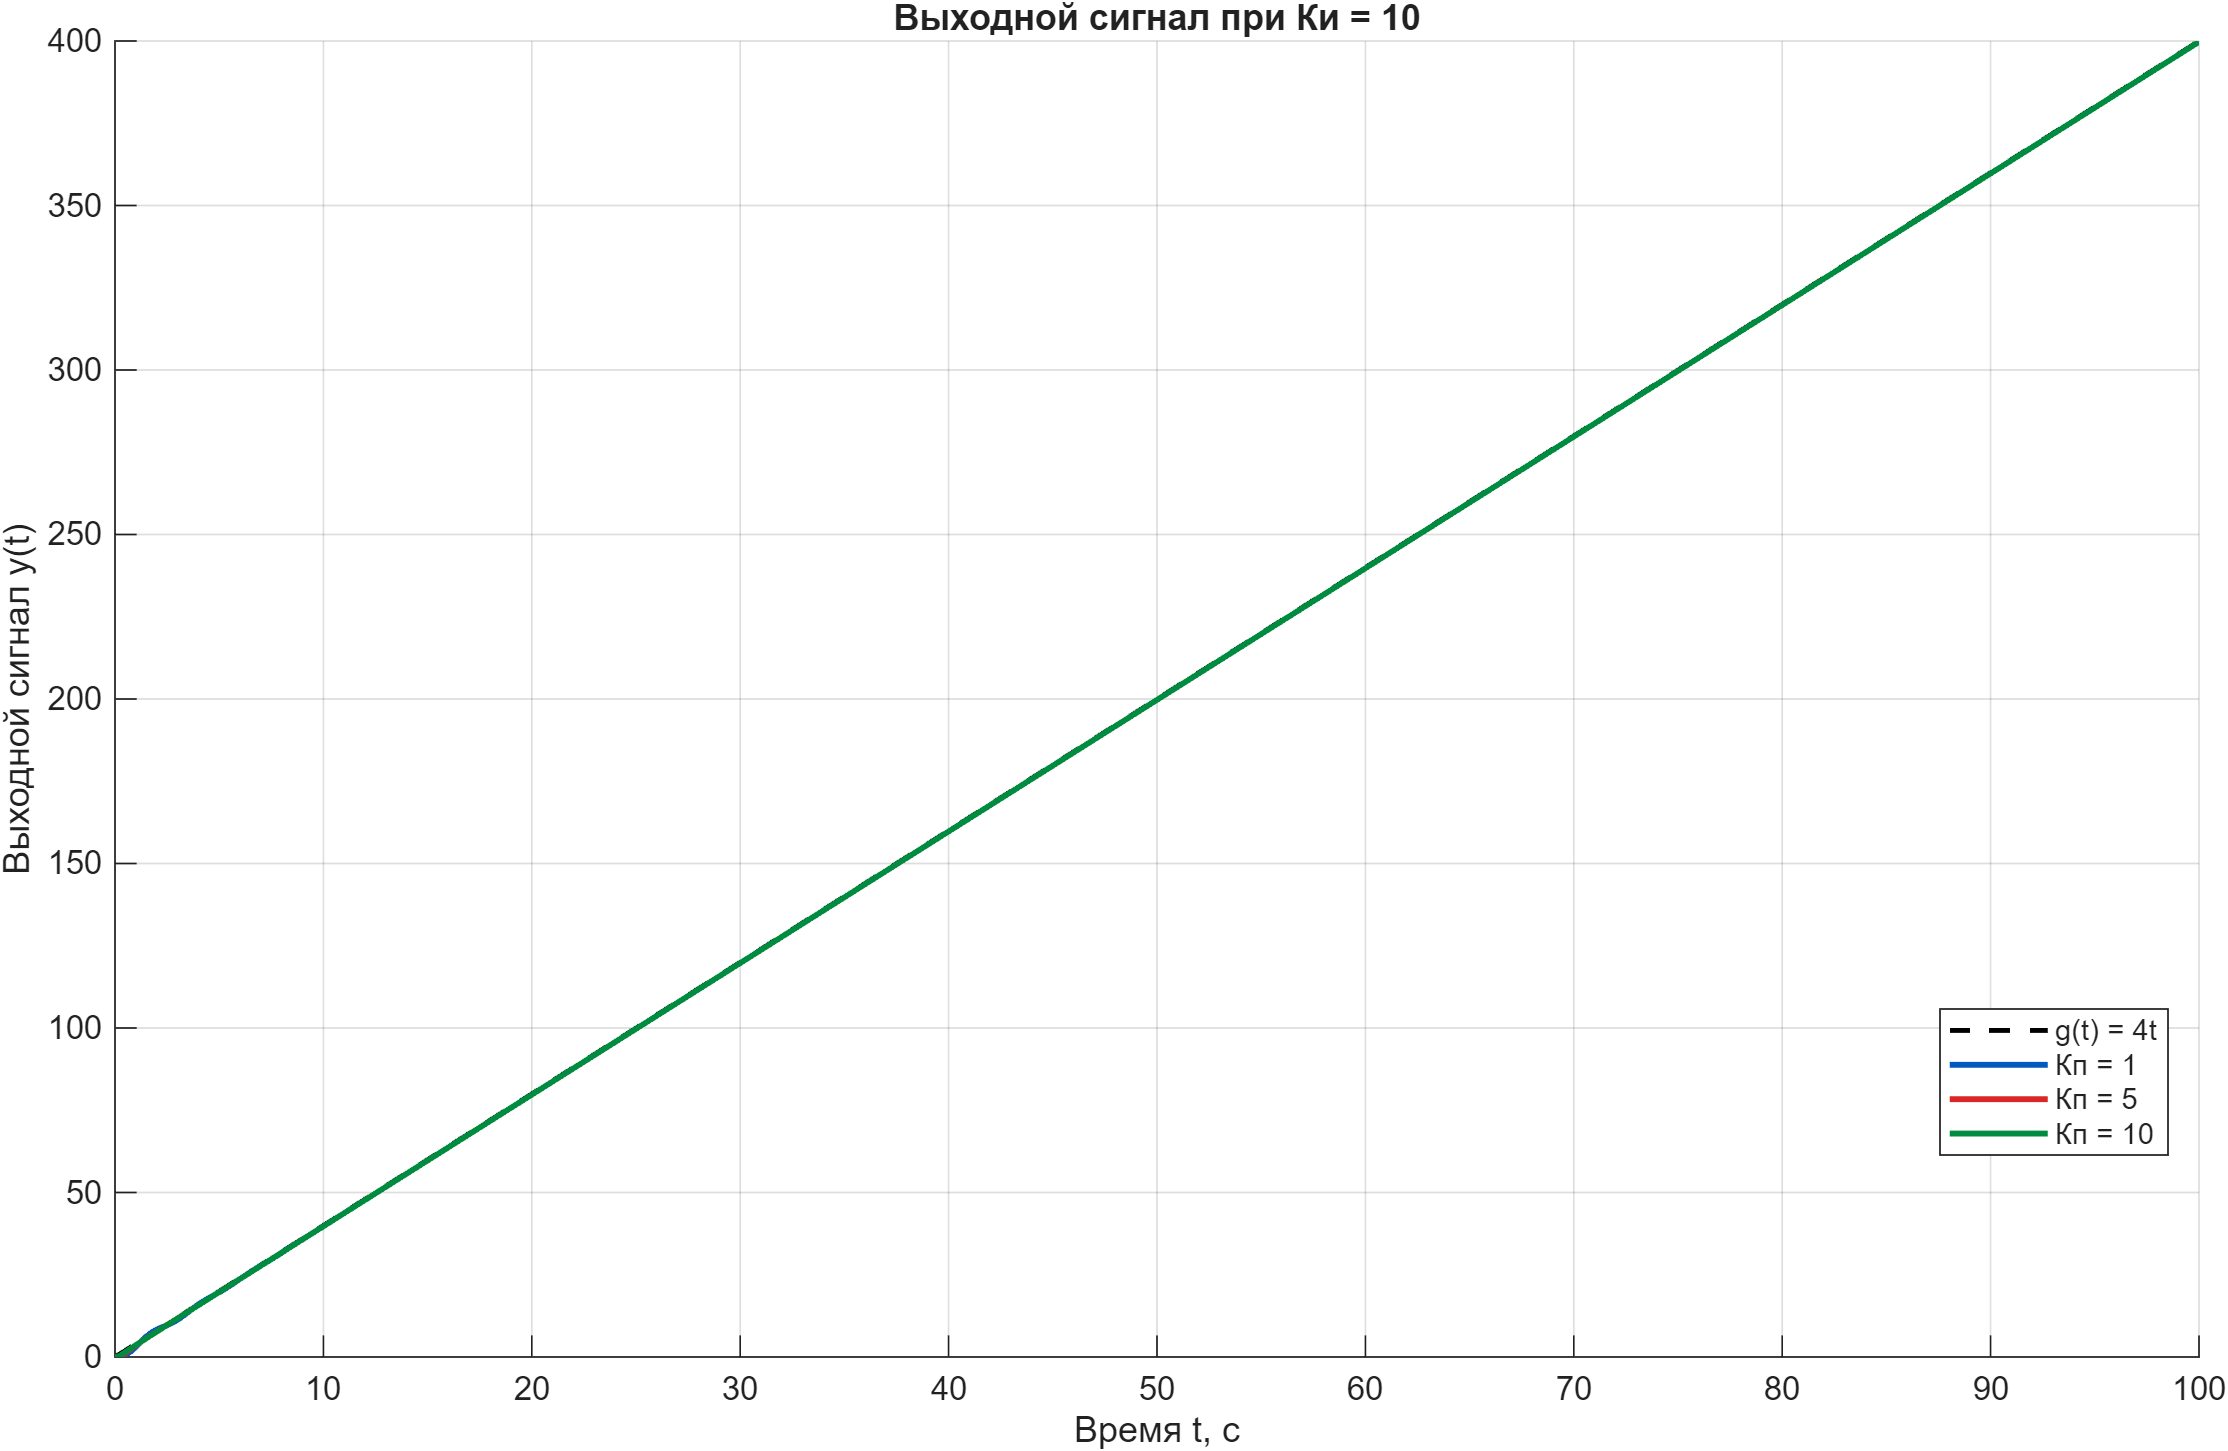
\includegraphics[width=0.85\textwidth]{res3/Lab5_Task3_Figure5.png}
    \caption{Переходные процессы выходного сигнала
    при $K_{\text{и}}=10$}
    \label{fig:task3_y_ki10}
\end{figure}

% -----------------------------------------------------------
% ГРАФИК 6 - e(t), Kи = 10
% -----------------------------------------------------------
\begin{figure}[H]
    \centering
    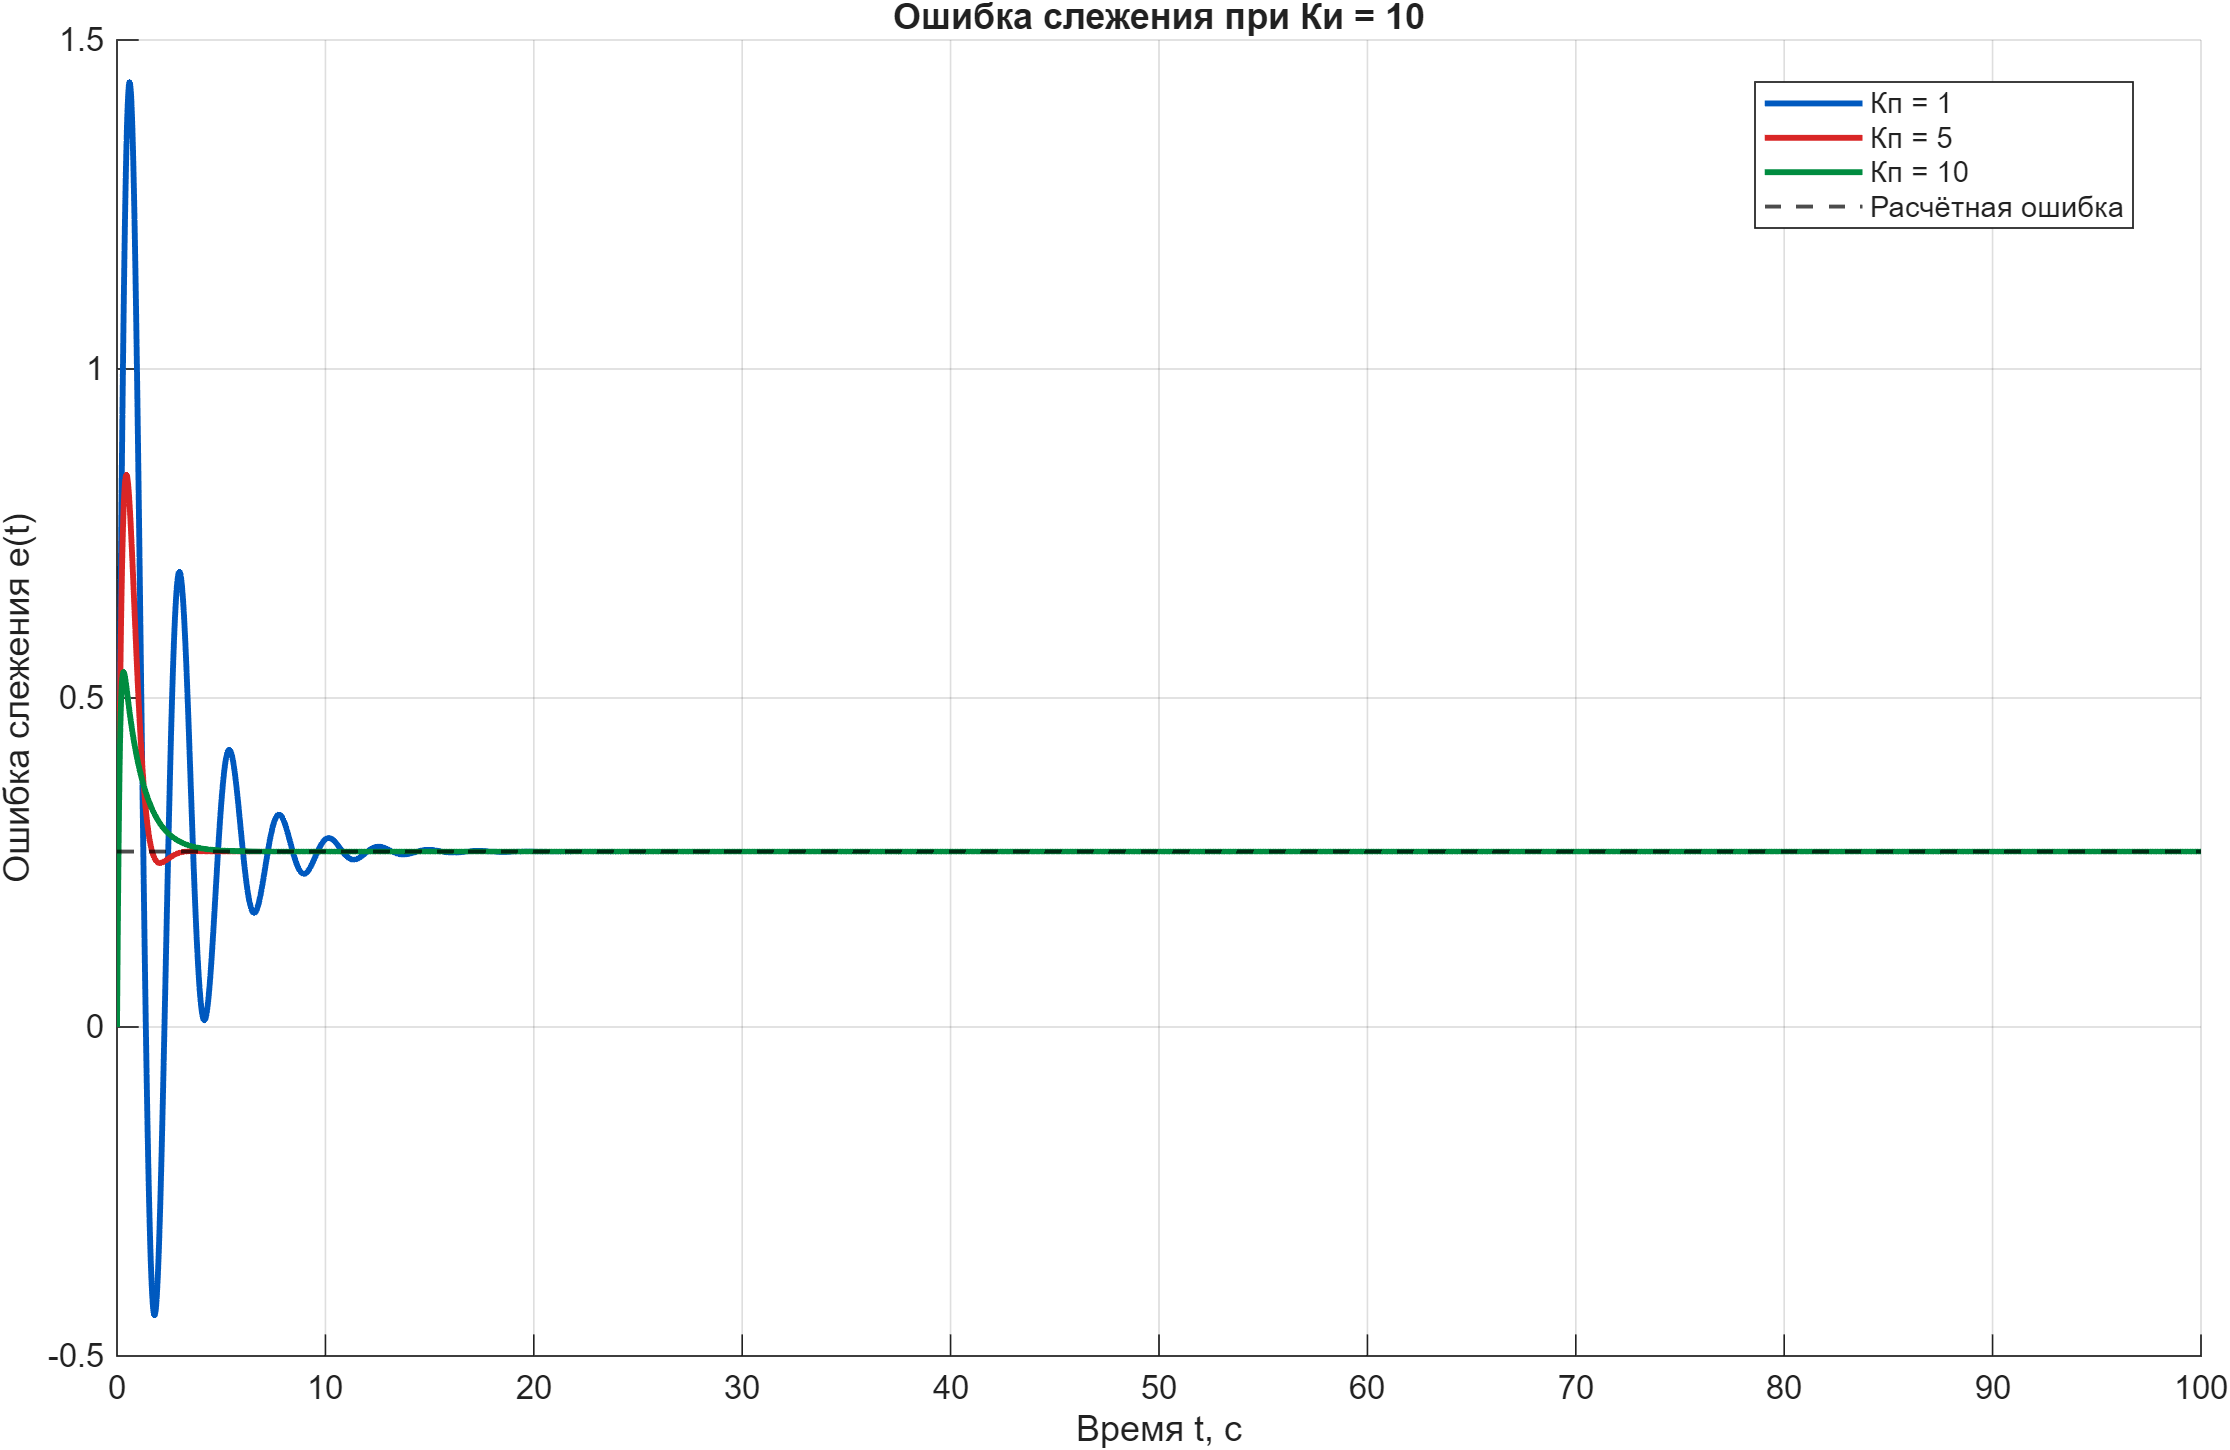
\includegraphics[width=0.85\textwidth]{res3/Lab5_Task3_Figure6.png}
    \caption{Переходные процессы ошибки слежения
    при $K_{\text{и}}=10$}
    \label{fig:task3_e_ki10}
\end{figure}

При $K_{\text{и}}=10$ установившаяся ошибка
имеет наименьшее значение среди
рассматриваемых групп экспериментов.


\subsection{Вывод по заданию 3}

В ходе выполнения задания исследованы
точностные свойства замкнутой системы
с пропорционально-интегральным регулятором.

Аналитически установлено, что при линейно
возрастающем задающем воздействии
$g(t)=4t$ установившаяся ошибка определяется
интегральным коэффициентом $K_{\text{и}}$.

Увеличение $K_{\text{и}}$ уменьшает
установившуюся ошибку слежения.

Пропорциональный коэффициент $K_{\text{п}}$
влияет на переходный процесс, однако
при фиксированном $K_{\text{и}}$
не изменяет установившуюся ошибку.

Таким образом, ПИ-регулятор обеспечивает
первый порядок астатизма и позволяет
изменять переходные характеристики системы
при сохранении заданной установившейся ошибки.





% ===========================================================
% ЗАДАНИЕ 4. ВНЕШНИЕ ВОЗМУЩЕНИЯ
% ===========================================================

\newpage
\section{Задание 4. Внешние возмущения}

\subsection{Исходные данные}

В соответствии с вариантом 3 используется
структурная схема а), представленная
на рисунке 6 методических указаний.

Передаточная функция объекта управления:
\[
    W(s)=\frac{1.5}{0.1s^2+2.2s+1}.
\]

В прямом контуре системы имеется
интегрирующее звено:
\[
    H(s)=\frac{1}{s}.
\]

Амплитуды внешних возмущений:
\[
    F_1=-0.5,\qquad F_2=1.
\]

Возмущения представляют собой ступенчатые
воздействия:
\[
    f_1(t)=-0.5\cdot1(t),
    \qquad f_2(t)=1(t).
\]

Задающее воздействие в обоих экспериментах:
\[
    g(t)=1(t).
\]

Исследуются два случая:
\begin{itemize}
    \item $f_1(t)=-0.5\cdot1(t)$, $f_2(t)=0$;
    \item $f_1(t)=0$, $f_2(t)=1(t)$.
\end{itemize}

Структурная схема исследуемой системы
представлена на рисунке~\ref{fig:task4_schema}.

% -----------------------------------------------------------
% СТРУКТУРНАЯ СХЕМА 6а
% -----------------------------------------------------------
\begin{figure}[H]
    \centering
    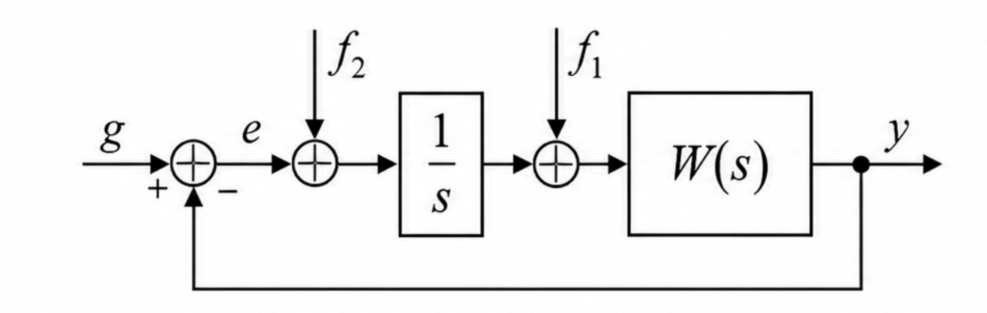
\includegraphics[width=0.85\textwidth]{res4/schema_task4.png}
    \caption{Структурная схема возмущённой
    системы управления (вариант 3, схема а)}
    \label{fig:task4_schema}
\end{figure}


\subsection{Передаточные функции системы}

На основании структурной схемы
ошибка слежения определяется выражением:
\[
    E(s)=G(s)-Y(s).
\]

Выходной сигнал системы:
\[
    Y(s)=W(s)
    \left[
        \frac{E(s)+F_2(s)}{s}+F_1(s)
    \right].
\]

Подставляя выражение для выходного сигнала
в уравнение ошибки, получим:
\[
    E(s)=G(s)-W(s)
    \left[
        \frac{E(s)+F_2(s)}{s}+F_1(s)
    \right].
\]

После преобразования:
\[
    \left(1+\frac{W(s)}{s}\right)E(s)
    =
    G(s)-W(s)F_1(s)
    -\frac{W(s)}{s}F_2(s).
\]

Следовательно:
\begin{equation}
    \boxed{
    E(s)=
    \frac{s}{s+W(s)}G(s)
    -\frac{sW(s)}{s+W(s)}F_1(s)
    -\frac{W(s)}{s+W(s)}F_2(s)
    }.
\end{equation}

Передаточные функции от задающего
воздействия и возмущений к ошибке:
\[
    W_{g\to e}(s)=\frac{s}{s+W(s)},
\]
\[
    W_{f_1\to e}(s)=
    -\frac{sW(s)}{s+W(s)},
\]
\[
    W_{f_2\to e}(s)=
    -\frac{W(s)}{s+W(s)}.
\]

Для удобства введём обозначение:
\[
    P(s)=0.1s^2+2.2s+1.
\]

Тогда:
\[
    W(s)=\frac{1.5}{P(s)}.
\]

Подставляя $W(s)$, получим:
\[
    W_{g\to e}(s)=
    \frac{sP(s)}{sP(s)+1.5},
\]
\[
    W_{f_1\to e}(s)=
    -\frac{1.5s}{sP(s)+1.5},
\]
\[
    W_{f_2\to e}(s)=
    -\frac{1.5}{sP(s)+1.5}.
\]

Характеристический полином системы:
\[
    D(s)=0.1s^3+2.2s^2+s+1.5.
\]

Все коэффициенты положительны, причём:
\[
    2.2\cdot1>0.1\cdot1.5.
\]

Таким образом, согласно критерию Гурвица,
замкнутая система асимптотически устойчива.


\subsection{Исследование влияния возмущения $f_1(t)$}

В первом эксперименте принимаем:
\[
    g(t)=1(t),\qquad
    f_1(t)=-0.5\cdot1(t),\qquad
    f_2(t)=0.
\]

Изображения Лапласа:
\[
    G(s)=\frac{1}{s},\qquad
    F_1(s)=-\frac{0.5}{s},\qquad
    F_2(s)=0.
\]

Изображение ошибки слежения:
\[
    E_1(s)=
    W_{g\to e}(s)G(s)
    +W_{f_1\to e}(s)F_1(s).
\]

После подстановки:
\[
    E_1(s)=
    \frac{sP(s)}{sP(s)+1.5}\frac{1}{s}
    -\frac{1.5s}{sP(s)+1.5}
    \left(-\frac{0.5}{s}\right).
\]

Упрощая выражение, получим:
\[
    E_1(s)=
    \frac{P(s)+0.75}{sP(s)+1.5}.
\]

Для определения предельного значения
установившейся ошибки воспользуемся
теоремой о предельном значении:
\[
    \varepsilon_1=
    \lim_{s\to0}sE_1(s).
\]

Следовательно:
\[
    \varepsilon_1=
    \lim_{s\to0}
    \frac{s(P(s)+0.75)}
    {sP(s)+1.5}.
\]

В результате:
\begin{equation}
    \boxed{\varepsilon_1=0}.
\end{equation}

Таким образом, постоянное возмущение
$f_1(t)$ полностью компенсируется
благодаря интегрирующему звену.

Для проверки результата проводится
моделирование переходного процесса
ошибки слежения.

% -----------------------------------------------------------
% ГРАФИК 1 - ВОЗМУЩЕНИЕ f1
% -----------------------------------------------------------
\begin{figure}[H]
    \centering
    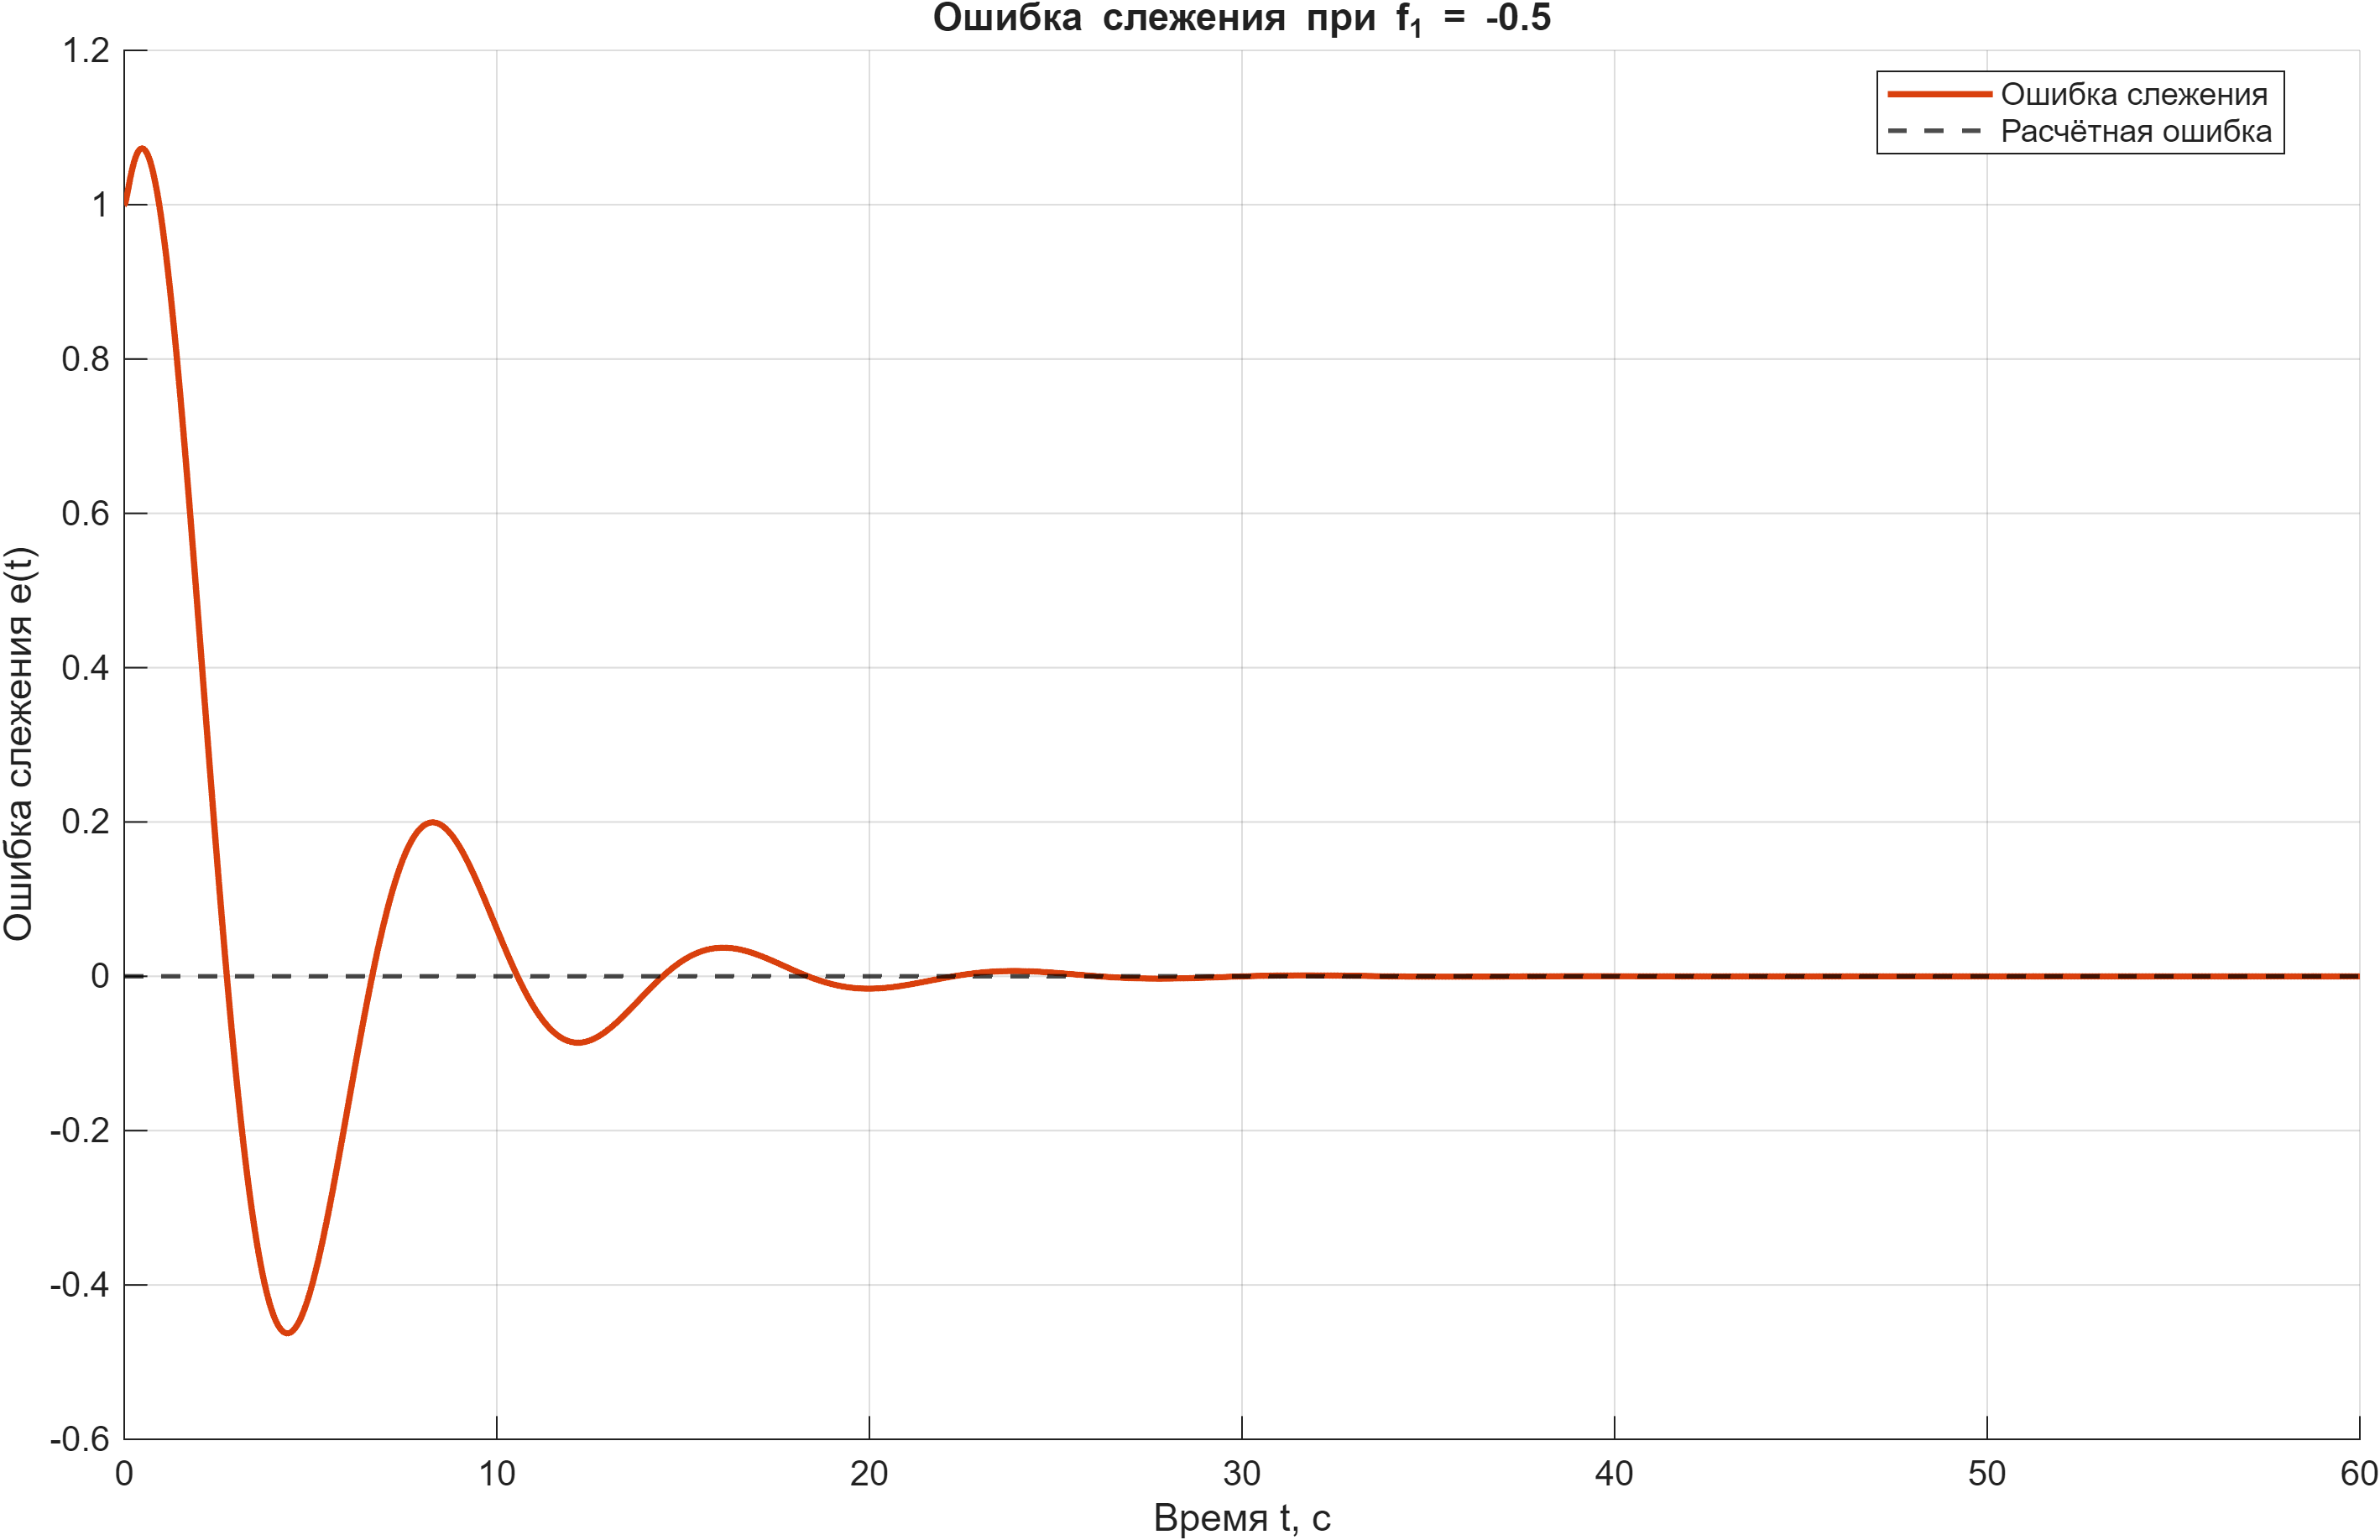
\includegraphics[width=0.85\textwidth]{res4/Lab5_Task4_Figure1.png}
    \caption{Переходный процесс ошибки слежения
    при $f_1(t)=-0.5\cdot1(t)$, $f_2(t)=0$}
    \label{fig:task4_error_f1}
\end{figure}


\subsection{Исследование влияния возмущения $f_2(t)$}

Во втором эксперименте принимаем:
\[
    g(t)=1(t),\qquad
    f_1(t)=0,\qquad
    f_2(t)=1(t).
\]

Изображения Лапласа:
\[
    G(s)=\frac{1}{s},\qquad
    F_1(s)=0,\qquad
    F_2(s)=\frac{1}{s}.
\]

Изображение ошибки слежения:
\[
    E_2(s)=
    W_{g\to e}(s)G(s)
    +W_{f_2\to e}(s)F_2(s).
\]

После подстановки:
\[
    E_2(s)=
    \frac{sP(s)}{sP(s)+1.5}\frac{1}{s}
    -\frac{1.5}{sP(s)+1.5}\frac{1}{s}.
\]

Упрощая выражение, получим:
\[
    E_2(s)=
    \frac{sP(s)-1.5}
    {s(sP(s)+1.5)}.
\]

Используя теорему о предельном значении:
\[
    \varepsilon_2=
    \lim_{s\to0}sE_2(s).
\]

Следовательно:
\[
    \varepsilon_2=
    \lim_{s\to0}
    \frac{sP(s)-1.5}{sP(s)+1.5}.
\]

В результате:
\begin{equation}
    \boxed{\varepsilon_2=-1}.
\end{equation}

Таким образом, возмущение $f_2(t)$
приводит к ненулевой установившейся
ошибке слежения.

Постоянное возмущение на входе
интегрирующего звена не компенсируется
интегральным действием системы.

Для проверки аналитического результата
проводится моделирование переходного
процесса ошибки слежения.

% -----------------------------------------------------------
% ГРАФИК 2 - ВОЗМУЩЕНИЕ f2
% -----------------------------------------------------------
\begin{figure}[H]
    \centering
    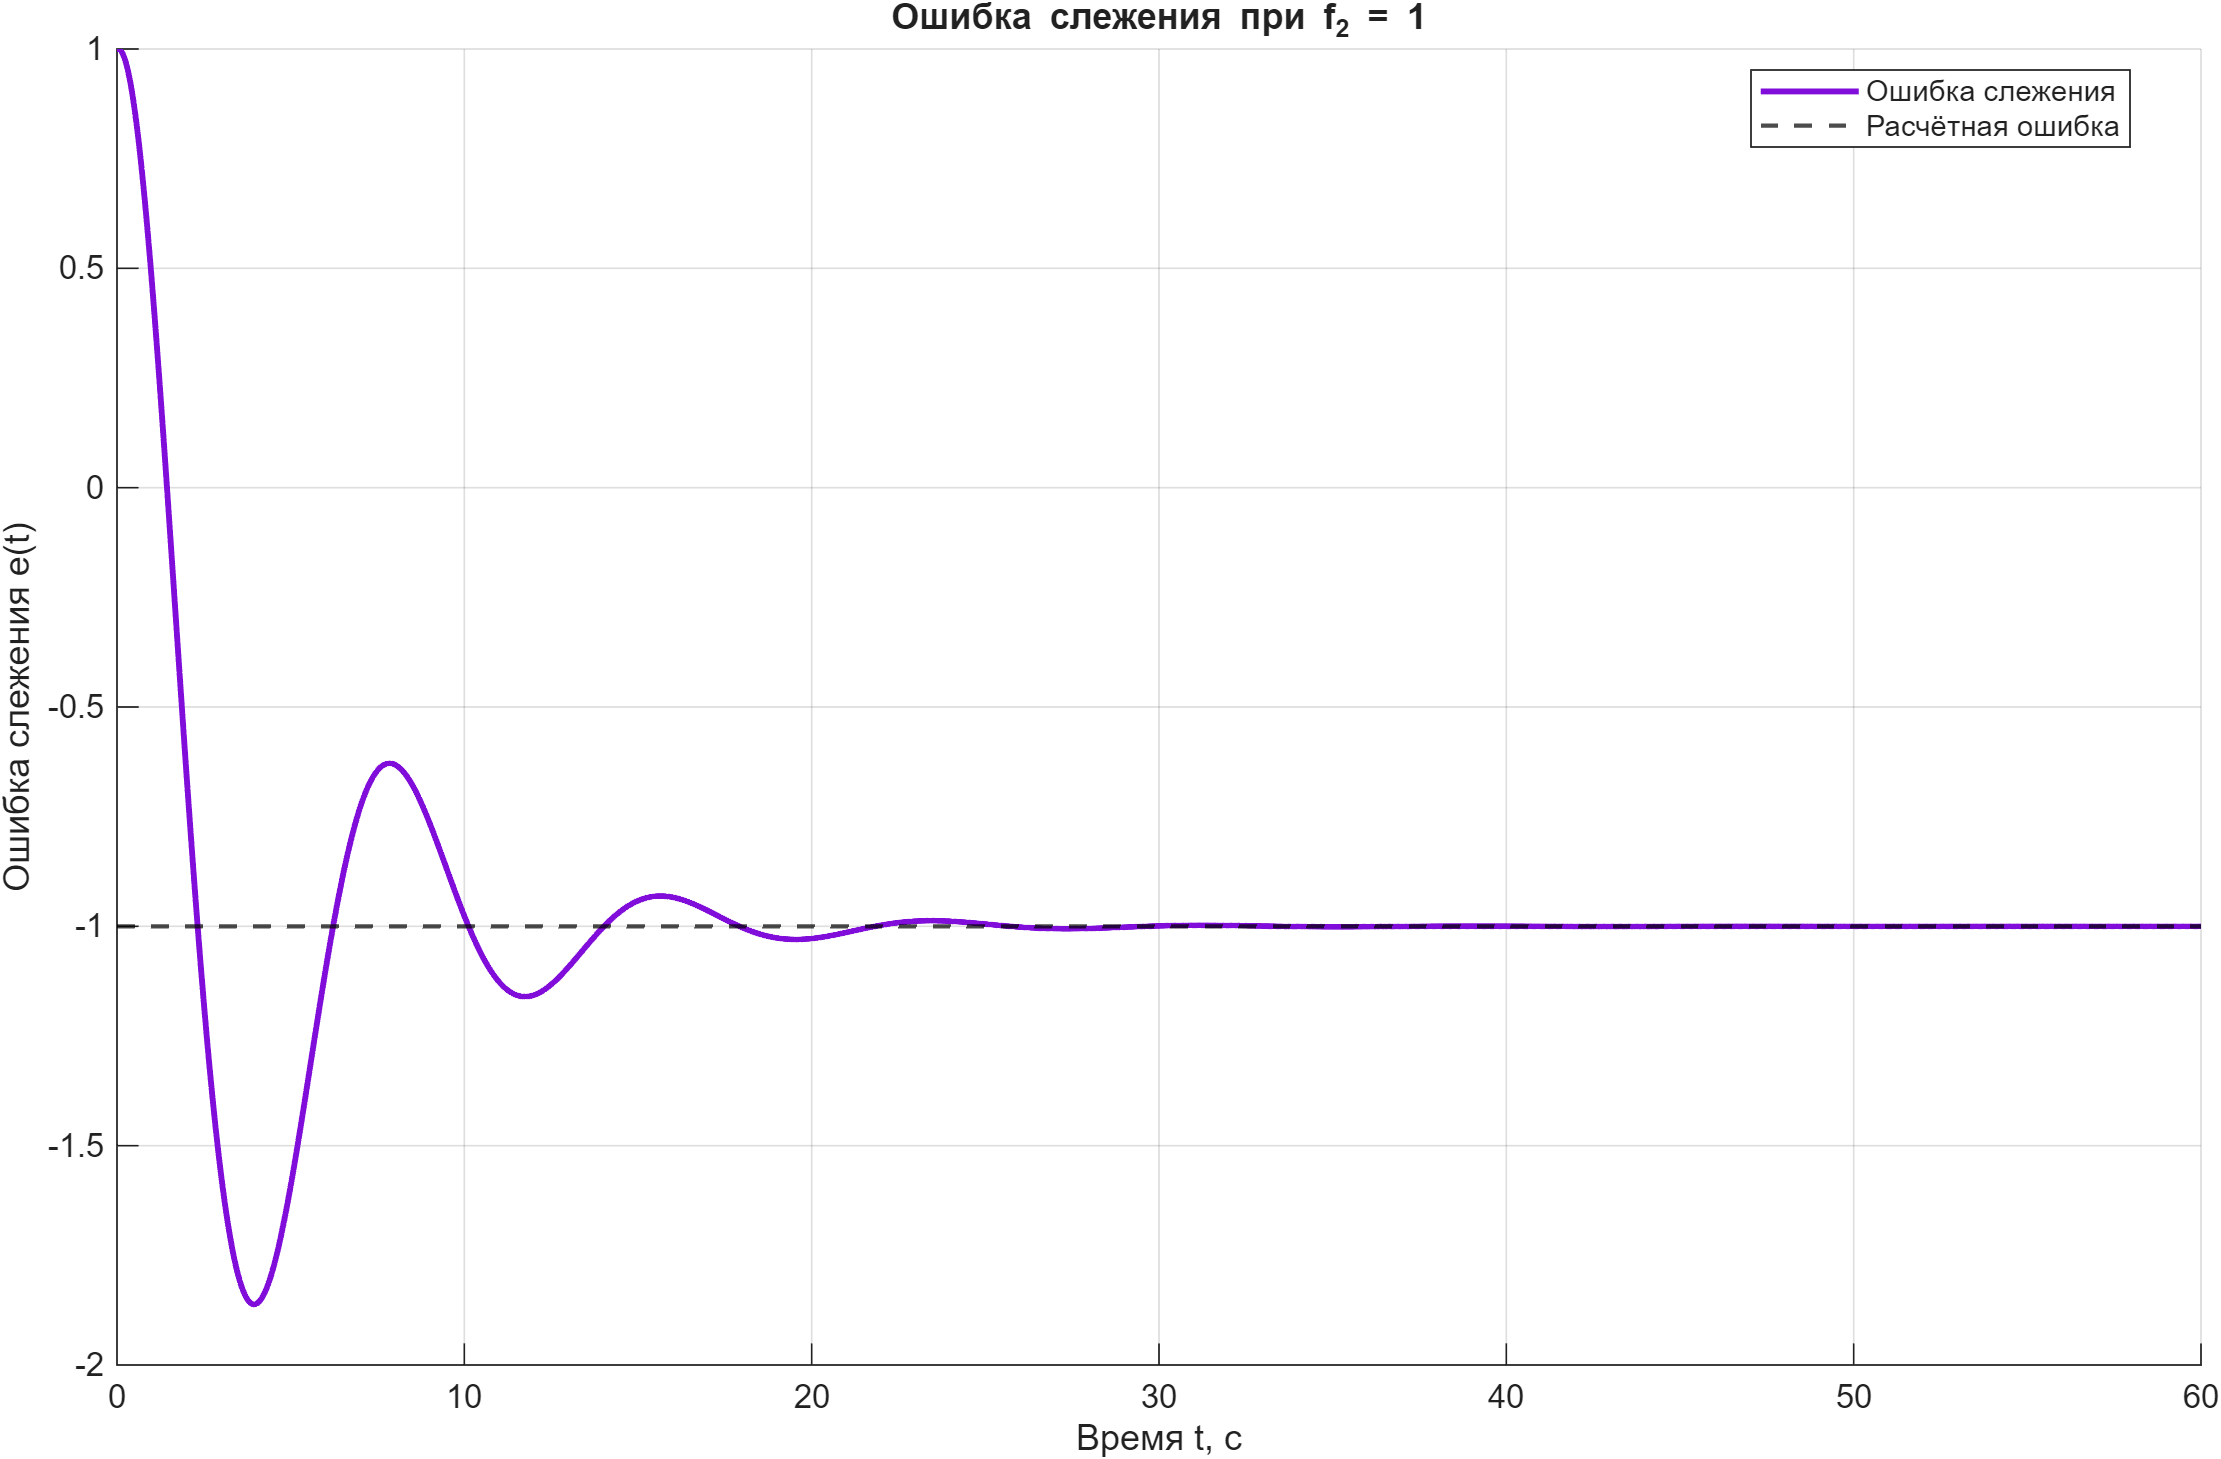
\includegraphics[width=0.85\textwidth]{res4/Lab5_Task4_Figure2.png}
    \caption{Переходный процесс ошибки слежения
    при $f_1(t)=0$, $f_2(t)=1(t)$}
    \label{fig:task4_error_f2}
\end{figure}


\subsection{Сравнение результатов}

Результаты аналитического расчёта
представлены в таблице~\ref{tab:task4_errors}.

\begin{table}[H]
    \centering
    \caption{Установившиеся ошибки
    при различных возмущениях}
    \label{tab:task4_errors}

    \setlength{\tabcolsep}{24pt}

    \begin{tabular}{ccc}
        \toprule
        Возмущение & Амплитуда & $\varepsilon$ \\
        \midrule
        $f_1(t)$ & $-0.5$ & $0$ \\
        $f_2(t)$ & $1$ & $-1$ \\
        \bottomrule
    \end{tabular}
\end{table}

Полученные результаты показывают,
что влияние внешнего возмущения
на установившуюся ошибку зависит
от точки его приложения
в структурной схеме системы.


\subsection{Вывод по заданию 4}

В ходе выполнения задания исследовано
влияние внешних возмущений на точностные
свойства замкнутой системы управления.

При действии постоянного возмущения
$f_1(t)=-0.5\cdot1(t)$ установившаяся
ошибка равна нулю. Это объясняется
наличием интегрирующего звена
в прямом контуре системы.

При действии возмущения
$f_2(t)=1(t)$ установившаяся
ошибка равна $-1$.

Следовательно, способность системы
компенсировать постоянные возмущения
зависит от места их приложения.

Наличие интегратора не гарантирует
нулевую установившуюся ошибку
для всех внешних возмущений.



% ===========================================================
% ЗАДАНИЕ 5. ПОЛИНОМИАЛЬНОЕ ВХОДНОЕ ВОЗДЕЙСТВИЕ
% ===========================================================

\newpage
\section{Задание 5. Полиномиальное входное воздействие}

\subsection{Исходные данные}

В соответствии с вариантом 3 передаточная
функция объекта управления имеет вид:
\[
    W(s)=\frac{1.5}{0.1s^2+2.2s+1}.
\]

Передаточная функция регулятора:
\[
    H(s)=1.
\]

Задающее воздействие выбирается
в соответствии с таблицей 5:
\begin{equation}
    \boxed{g(t)=2+0.5t}.
\end{equation}

Рассматривается замкнутая система управления
с единичной отрицательной обратной связью.

Ошибка слежения определяется выражением:
\[
    e(t)=g(t)-y(t).
\]

Необходимо определить установившуюся
составляющую ошибки слежения аналитически,
используя первые три члена ряда Тейлора,
и сравнить полученное выражение
с результатами моделирования.

Структурная схема исследуемой системы
представлена на рисунке~\ref{fig:task5_schema}.

% -----------------------------------------------------------
% СТРУКТУРНАЯ СХЕМА
% -----------------------------------------------------------
\begin{figure}[H]
    \centering
    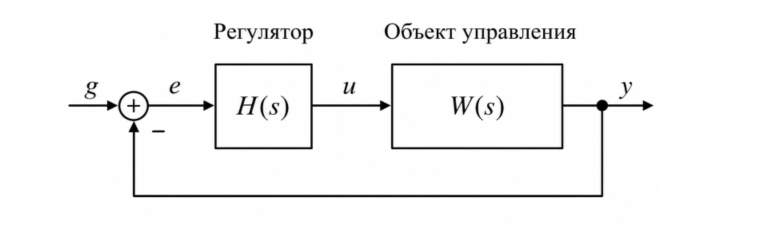
\includegraphics[width=0.85\textwidth]{schema_task1.png}
    \caption{Структурная схема замкнутой системы
    при $H(s)=1$}
    \label{fig:task5_schema}
\end{figure}


\subsection{Передаточные функции системы}

Передаточная функция разомкнутой системы:
\[
    L(s)=H(s)W(s)=W(s).
\]

Передаточная функция замкнутой системы
по задающему воздействию:
\[
    T(s)=\frac{L(s)}{1+L(s)}.
\]

После подстановки получим:
\begin{equation}
    \boxed{
    T(s)=
    \frac{1.5}{0.1s^2+2.2s+2.5}
    }.
\end{equation}

Передаточная функция замкнутой системы
по ошибке:
\[
    W_{g\to e}(s)=\frac{1}{1+W(s)}.
\]

Следовательно:
\begin{equation}
    \boxed{
    W_{g\to e}(s)=
    \frac{0.1s^2+2.2s+1}
    {0.1s^2+2.2s+2.5}
    }.
\end{equation}

Характеристический полином замкнутой системы:
\[
    D(s)=0.1s^2+2.2s+2.5.
\]

Все коэффициенты характеристического
полинома второго порядка положительны.
Следовательно, замкнутая система
асимптотически устойчива.


\subsection{Аналитическое определение
установившейся ошибки}

Для определения установившейся составляющей
ошибки используем разложение передаточной
функции по ошибке в ряд Тейлора
в окрестности точки $s=0$.

Сохраняя первые три члена ряда, получим:
\begin{equation}
    W_{g\to e}(s)=
    c_0+c_1s+\frac{c_2}{2}s^2+O(s^3).
\end{equation}

Коэффициенты ошибок определяются
по формулам:
\[
    c_i=
    \left.
    \frac{d^iW_{g\to e}(s)}{ds^i}
    \right|_{s=0}.
\]

Нулевой коэффициент:
\[
    c_0=W_{g\to e}(0)
    =\frac{1}{2.5}=0.4.
\]

Первый коэффициент:
\[
    c_1=
    \left.
    \frac{dW_{g\to e}(s)}{ds}
    \right|_{s=0}.
\]

Для вычисления производной используем:
\[
    W_{g\to e}(s)=
    1-\frac{1.5}{0.1s^2+2.2s+2.5}.
\]

Тогда:
\[
    c_1=
    \frac{1.5\cdot2.2}{2.5^2}
    =0.528.
\]

Второй коэффициент:
\[
    c_2=
    \left.
    \frac{d^2W_{g\to e}(s)}{ds^2}
    \right|_{s=0}.
\]

После дифференцирования:
\[
    c_2=
    \frac{2\cdot1.5\cdot0.1}{2.5^2}
    -
    \frac{2\cdot1.5\cdot2.2^2}{2.5^3}.
\]

Следовательно:
\[
    c_2=-0.88128.
\]

Таким образом, разложение передаточной
функции по ошибке имеет вид:
\[
    W_{g\to e}(s)\approx
    0.4+0.528s-0.44064s^2.
\]

В соответствии с методом коэффициентов
ошибок установившаяся составляющая
ошибки слежения определяется выражением:
\begin{equation}
    e_y(t)=
    c_0g(t)+c_1\dot{g}(t)
    +\frac{c_2}{2}\ddot{g}(t).
\end{equation}

Для задающего воздействия:
\[
    g(t)=2+0.5t
\]

производные равны:
\[
    \dot{g}(t)=0.5,
    \qquad
    \ddot{g}(t)=0.
\]

Подставляя полученные значения:
\[
    e_y(t)=
    0.4(2+0.5t)
    +0.528\cdot0.5
    -0.44064\cdot0.
\]

В результате получим:
\begin{equation}
    \boxed{
    e_y(t)=0.2t+1.064
    }.
\end{equation}

Полученное выражение показывает,
что установившаяся составляющая ошибки
линейно возрастает со временем.

Поскольку система обладает нулевым
порядком астатизма, она не обеспечивает
ограниченную ошибку слежения
при линейно возрастающем воздействии.


\subsection{Моделирование замкнутой системы}

Для проверки аналитических результатов
проводится моделирование замкнутой системы
при задающем воздействии $g(t)=2+0.5t$.

Сначала определяются переходные процессы
задающего воздействия и выходного сигнала.

% -----------------------------------------------------------
% ГРАФИК 1 - g(t) и y(t)
% -----------------------------------------------------------
\begin{figure}[H]
    \centering
    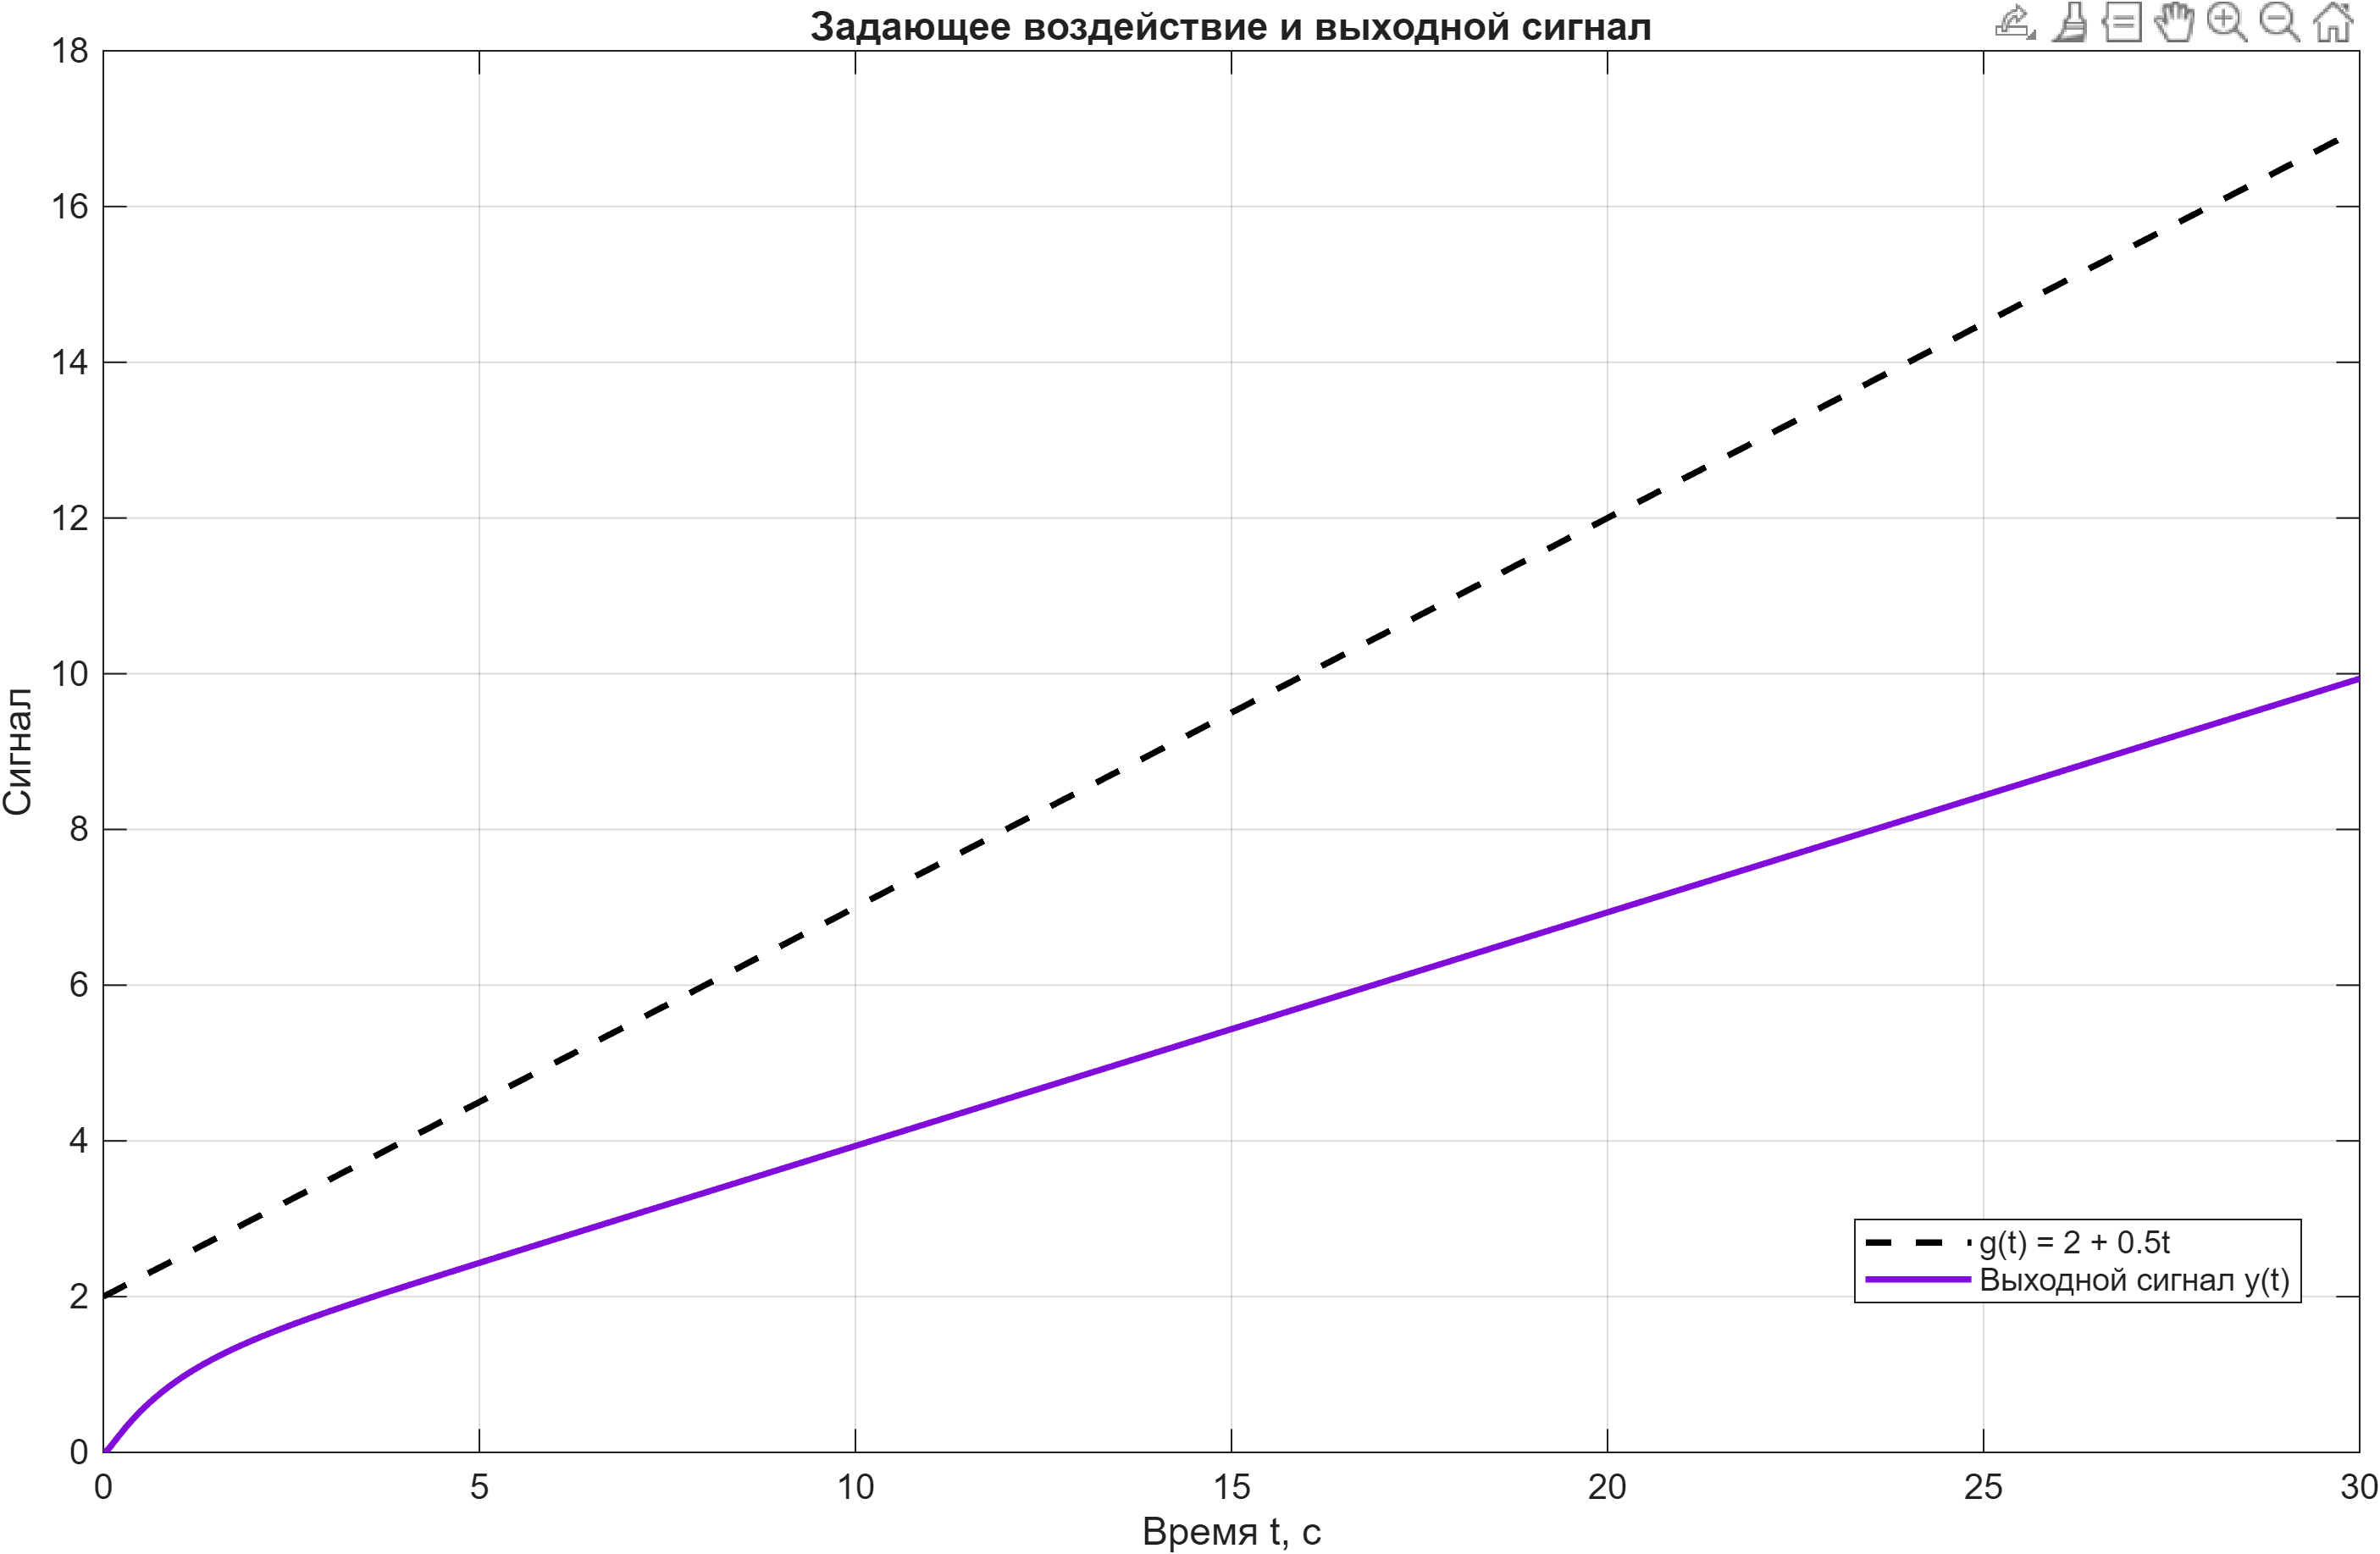
\includegraphics[width=0.85\textwidth]{res5/Lab5_Task5_Figure1.png}
    \caption{Сравнение задающего воздействия
    и выходного сигнала системы}
    \label{fig:task5_output}
\end{figure}

Ошибка слежения вычисляется
как разность между задающим воздействием
и выходным сигналом:
\[
    e(t)=g(t)-y(t).
\]

% -----------------------------------------------------------
% ГРАФИК 2 - Ошибка моделирования
% -----------------------------------------------------------
\begin{figure}[H]
    \centering
    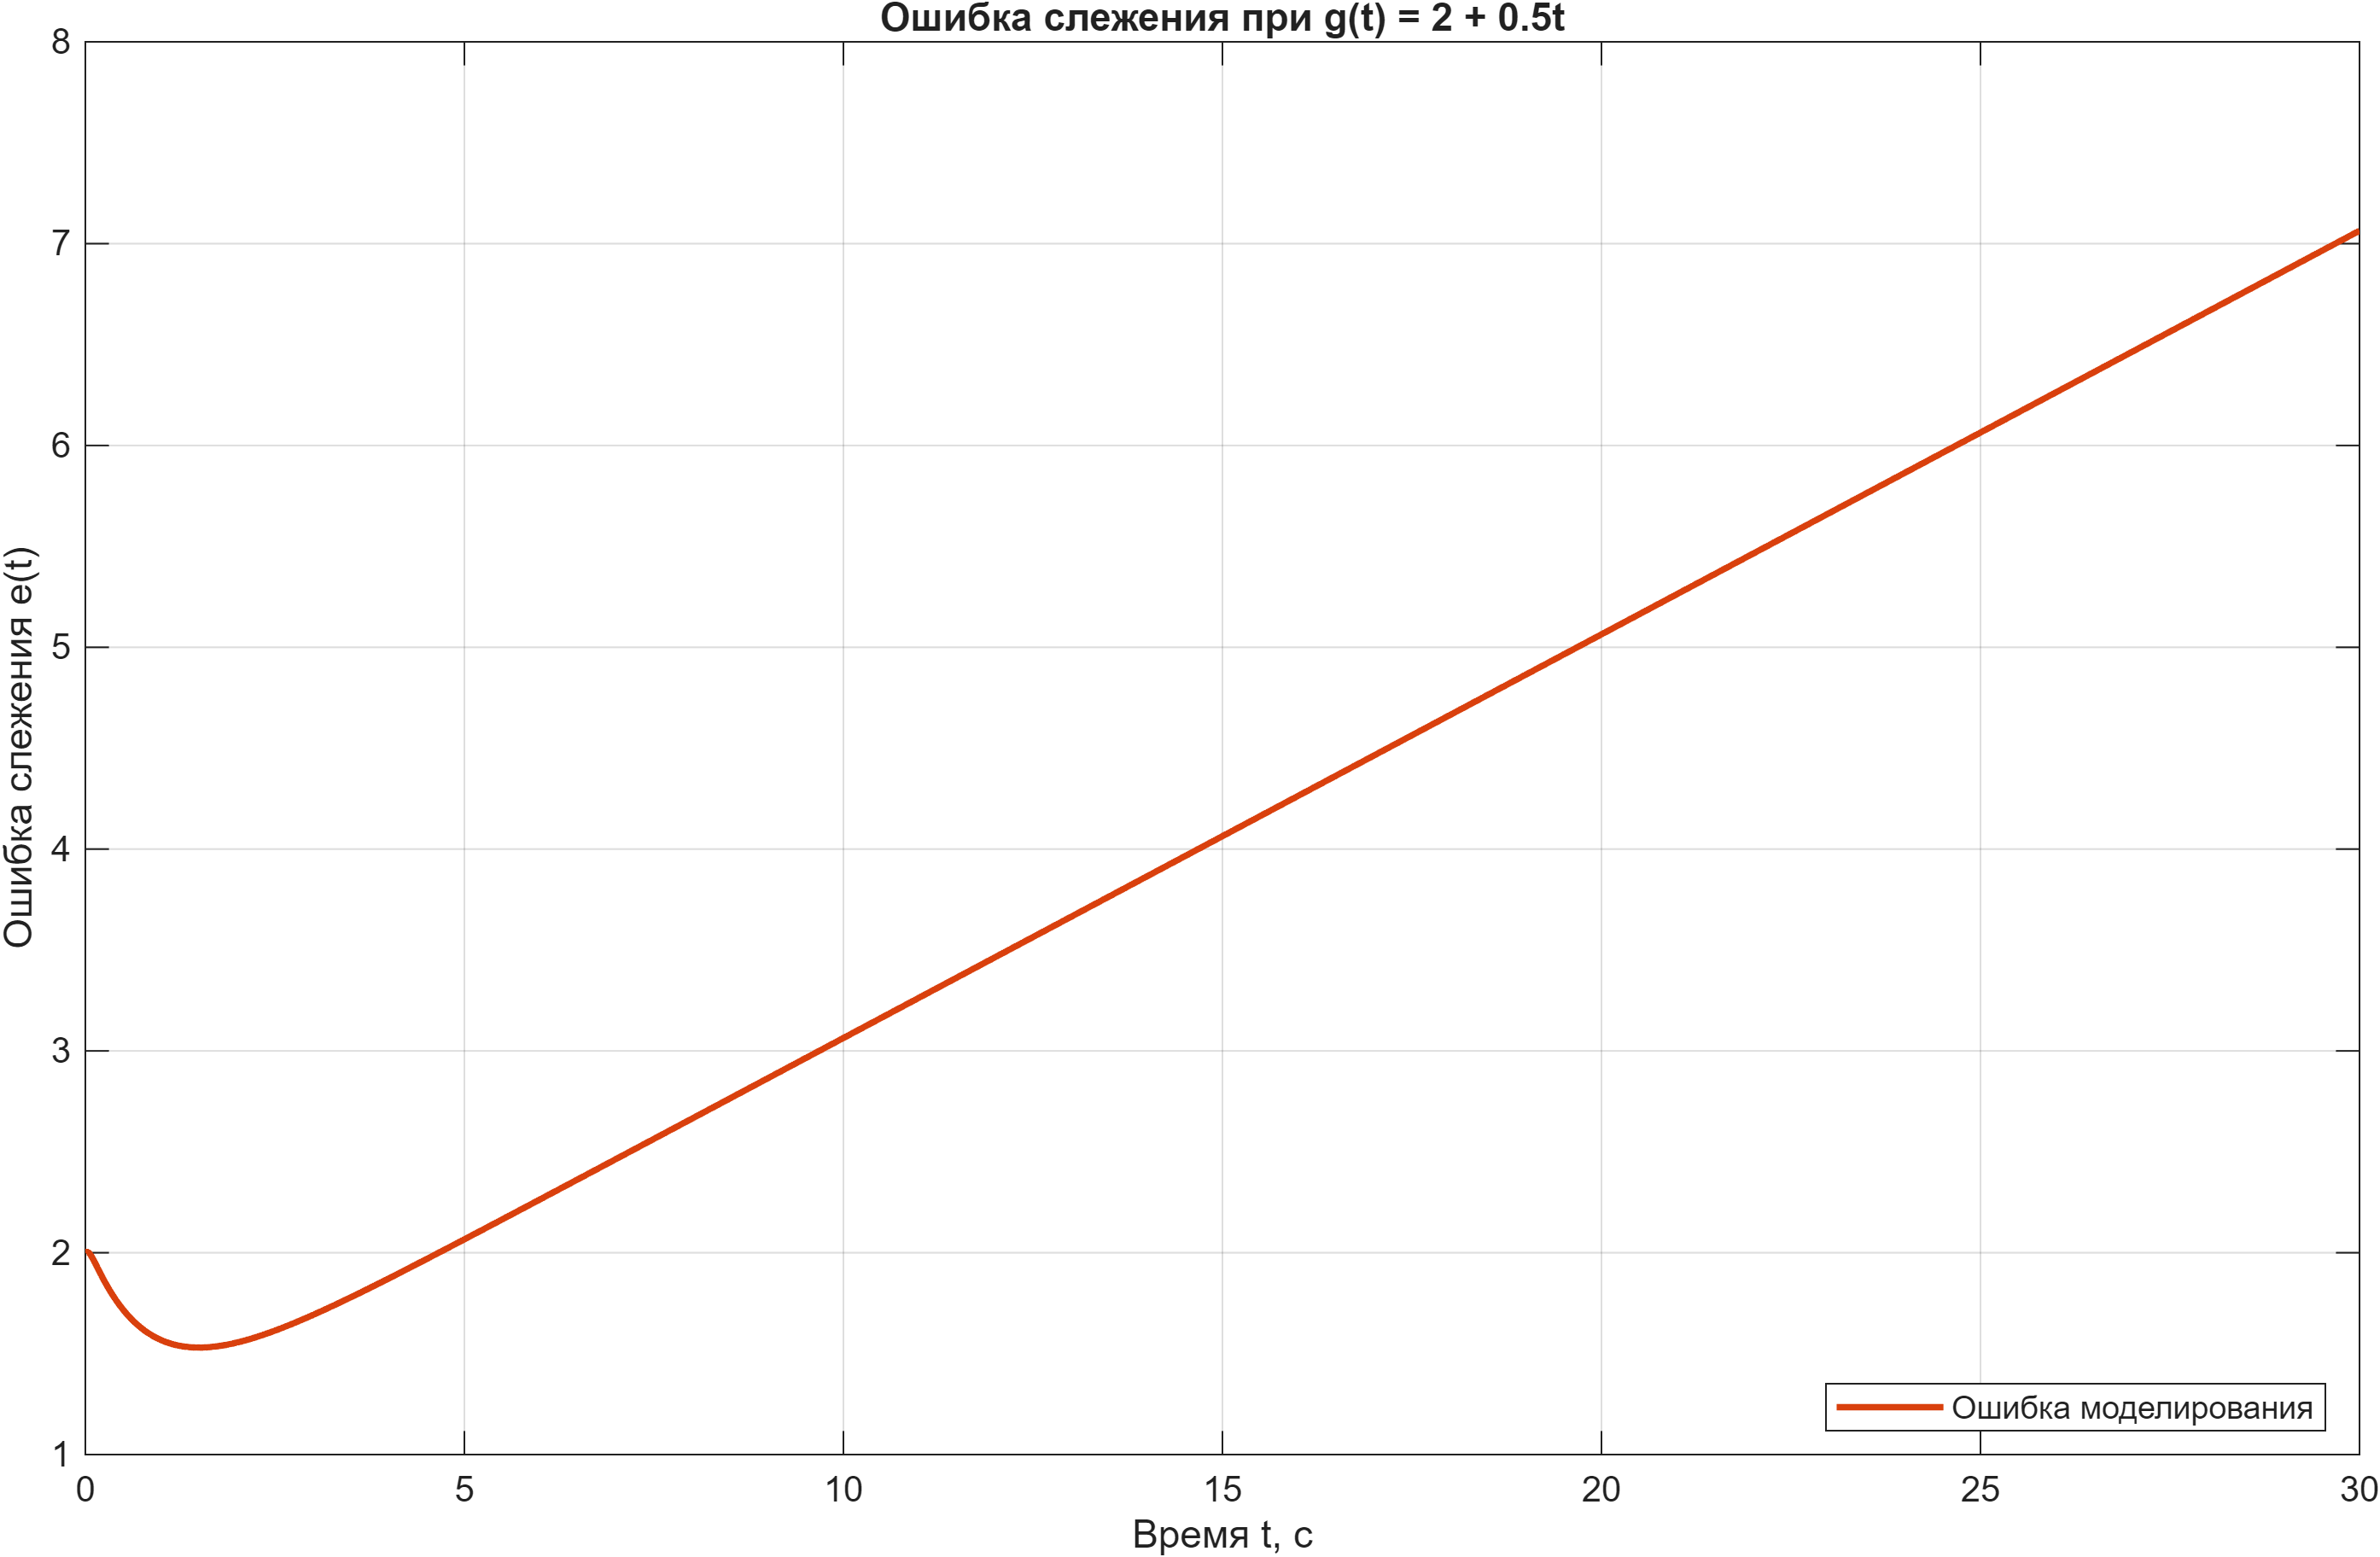
\includegraphics[width=0.85\textwidth]{res5/Lab5_Task5_Figure2.png}
    \caption{Ошибка слежения, полученная
    в результате моделирования}
    \label{fig:task5_error}
\end{figure}


\subsection{Сравнение аналитических
и экспериментальных результатов}

Для сравнения используем аналитически
полученное выражение установившейся ошибки:
\[
    e_y(t)=0.2t+1.064.
\]

На одном графике представлены ошибка
слежения, определённая моделированием,
и её аналитическая установившаяся составляющая.

% -----------------------------------------------------------
% ГРАФИК 3 - Сравнение ошибок
% -----------------------------------------------------------
\begin{figure}[H]
    \centering
    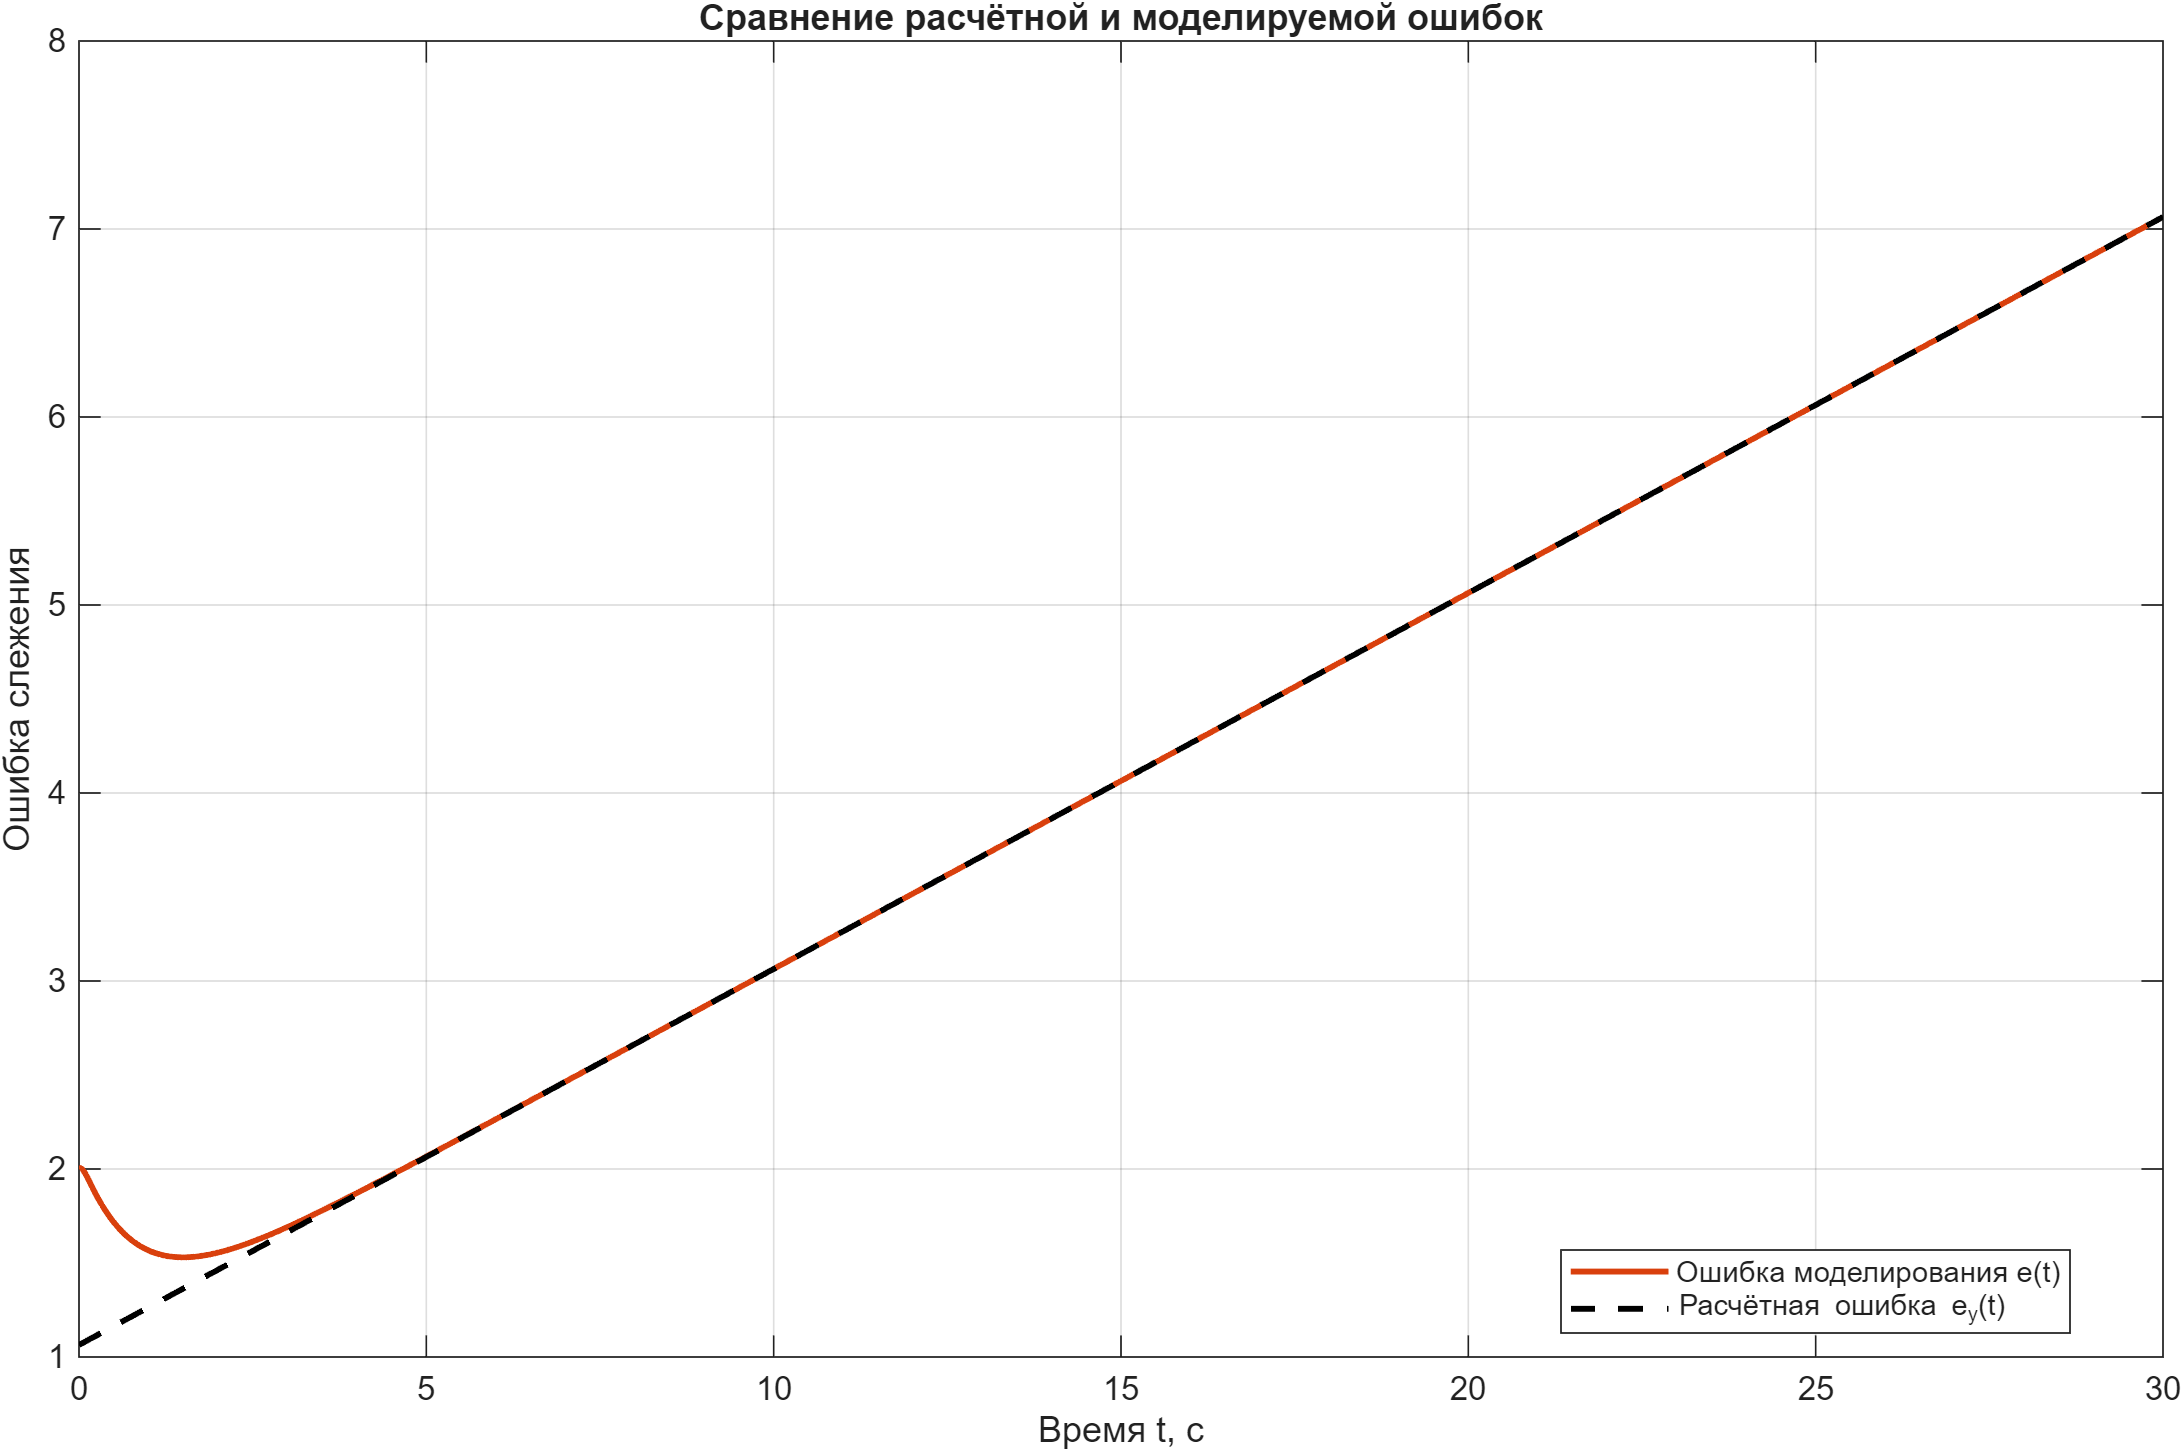
\includegraphics[width=0.85\textwidth]{res5/Lab5_Task5_Figure3.png}
    \caption{Сравнение расчётной
    и экспериментальной ошибок слежения}
    \label{fig:task5_comparison}
\end{figure}

В начальный момент времени результаты
моделирования отличаются от аналитической
установившейся составляющей из-за
наличия переходного процесса.

По мере затухания переходной составляющей
ошибка слежения приближается к
аналитически полученной зависимости.

Таким образом, метод коэффициентов ошибок
позволяет определить установившуюся
составляющую ошибки для полиномиального
задающего воздействия.


\subsection{Вывод по заданию 5}

В ходе выполнения задания исследованы
точностные свойства замкнутой системы
при полиномиальном задающем воздействии.

С использованием разложения передаточной
функции по ошибке в ряд Тейлора
получено аналитическое выражение:
\[
    e_y(t)=0.2t+1.064.
\]

При линейно возрастающем задающем
воздействии установившаяся составляющая
ошибки также линейно возрастает.

После затухания переходных процессов
результаты моделирования согласуются
с аналитическим расчётом.

Таким образом, система с нулевым порядком
астатизма не обеспечивает ограниченную
ошибку слежения при линейно
возрастающем задающем воздействии.




% ===========================================================
% ЗАКЛЮЧЕНИЕ
% ===========================================================

\newpage
\section{Заключение}

В ходе выполнения лабораторной работы №5 были
исследованы точностные свойства линейных
систем автоматического управления при
различных задающих воздействиях и внешних
возмущениях.

В первом задании исследована система
с пропорциональным регулятором.
Установлено, что увеличение коэффициента
усиления приводит к уменьшению ошибки
слежения, однако не обеспечивает
её полного устранения.
Система обладает нулевым порядком
астатизма.

Во втором задании исследована система
с интегральным регулятором.
Показано, что при постоянном задающем
воздействии установившаяся ошибка
равна нулю, а при линейно возрастающем
воздействии имеет конечное значение.
При квадратично возрастающем воздействии
ошибка неограниченно возрастает.
Таким образом, интегральный регулятор
обеспечивает первый порядок астатизма.

В третьем задании исследована система
с пропорционально-интегральным регулятором.
Установлено, что интегральный коэффициент
определяет величину установившейся ошибки,
а пропорциональный коэффициент влияет
на характер переходного процесса.
При фиксированном интегральном
коэффициенте изменение пропорционального
коэффициента не изменяет установившуюся
ошибку при линейном задающем воздействии.

В четвёртом задании исследовано влияние
внешних возмущений на точность управления.
Показано, что способность системы
компенсировать постоянные возмущения
зависит от точки их приложения.
Для рассматриваемой структуры
получены установившиеся ошибки
$\varepsilon_1=0$ и $\varepsilon_2=-1$.

В пятом задании исследована система
при полиномиальном задающем воздействии.
С использованием разложения передаточной
функции по ошибке в ряд Тейлора
получено аналитическое выражение
установившейся составляющей ошибки:
\[
    e_y(t)=0.2t+1.064.
\]

Полученные аналитические результаты
согласуются с теоретическими свойствами
исследуемых систем и позволяют объяснить
характер наблюдаемых переходных процессов.

Таким образом, точность системы управления
зависит от структуры регулятора,
его параметров, характера задающего
воздействия и места приложения
внешних возмущений.


\end{document}


